%% =====================================================================
%% Dissertacao de mestrado -- primeira versao integral (rascunho).
%%
%% Este arquivo e o documento principal da DISSERTACAO. Ele nao substitui
%% modeloABNT2.tex, que permanece como o texto da QUALIFICACAO: os dois
%% coexistem no mesmo diretorio e compartilham a classe, as figuras e a
%% bibliografia. Compile com:
%%
%%     pdflatex dissertacao && bibtex dissertacao && pdflatex dissertacao
%%
%% Baseado em modeloABNT2, v1.0 athila -- Copyright 2013 by Athila e Monaro
%% =====================================================================

% ------------------------------------------------------------------------
% Opcoes:
% 	tesedr:     Formata documento para tese de doutorado
%	qualidr:    Formata documento para qualificacao de doutorado
% 	dissertmst: Formata documento para dissertacao de mestrado
% 	qualimst:   Formata documento para qualificacao de mestrado
% ------------------------------------------------------------------------
\documentclass[dissertmst]{ufscar}

% ---
% PACOTES
% ---

% ---
% Pacotes fundamentais
% ---
\usepackage{cmap}				% Mapear caracteres especiais no PDF
\usepackage{lmodern}				% Usa a fonte Latin Modern
\usepackage{amsmath,amssymb}		% Carregado antes do hyperref, por convenção
\usepackage{makeidx}            	% Cria o indice
\usepackage{hyperref}  			% Controla a formação do índice
\usepackage{lastpage}			% Usado pela Ficha catalográfica
\usepackage{indentfirst}			% Indenta o primeiro parágrafo de cada seção.
\usepackage{nomencl} 			% Lista de simbolos
\usepackage{graphicx}			% Inclusão de gráficos
\usepackage[round]{natbib}
% \bibliographystyle{dinat}

%\usepackage[alf]{abntex2cite}
% ---

% ---
% Pacotes adicionais
% ---
\usepackage[printonlyused]{acronym}
\usepackage[table]{xcolor}
\usepackage{booktabs}
\usepackage{multirow}
\usepackage{tikz}
\usetikzlibrary{arrows.meta,positioning}
\usepackage{pgfplots}
\pgfplotsset{compat=1.16}
% ---

% ---
% Ambiente de algoritmo. A classe ufscar ja carrega `algorithm' e
% `algorithmic'; aqui apenas traduzimos as palavras-chave e o nome do
% flutuante para o portugues.
% ---
\floatname{algorithm}{Algoritmo}
\renewcommand{\algorithmicrequire}{\textbf{Entrada:}}
\renewcommand{\algorithmicensure}{\textbf{Saída:}}
\renewcommand{\algorithmicfor}{\textbf{para}}
\renewcommand{\algorithmicforall}{\textbf{para cada}}
\renewcommand{\algorithmicdo}{\textbf{faça}}
\renewcommand{\algorithmicendfor}{\textbf{fim para}}
\renewcommand{\algorithmicif}{\textbf{se}}
\renewcommand{\algorithmicthen}{\textbf{então}}
\renewcommand{\algorithmicelse}{\textbf{senão}}
\renewcommand{\algorithmicendif}{\textbf{fim se}}
\renewcommand{\algorithmicwhile}{\textbf{enquanto}}
\renewcommand{\algorithmicendwhile}{\textbf{fim enquanto}}
\renewcommand{\algorithmicrepeat}{\textbf{repita}}
\renewcommand{\algorithmicuntil}{\textbf{até que}}
% `\algorithmicreturn' só existe em versões recentes de algorithmic.sty; o
% \providecommand garante que o \renewcommand seguinte não falhe.
\providecommand{\algorithmicreturn}{\textbf{retorne}}
\renewcommand{\algorithmicreturn}{\textbf{retorne}}
% ---

% ---
% Abreviacoes de simbolos usadas com frequencia no texto.
% ---
\newcommand{\mpts}{m_{pts}}
\newcommand{\kmax}{k_{max}}
\newcommand{\coredist}{\mathrm{core}}
\newcommand{\mrd}{\mathrm{mrd}}
\newcommand{\ef}{\mathit{ef}}
% ---

% ---
% Informações de dados para CAPA e FOLHA DE ROSTO
% ---
%
% Título:
%	1. Título em português
%	2. Título em inglês
\titulo{CORE-SG multi-GPU: construção escalável de grafos baseados em densidade por decomposição em instâncias independentes}{Multi-GPU CORE-SG: scalable construction of density-based graphs by decomposition into independent instances}
%
% Autor:
%	1. Nome completo do autor
%	2. Formato de nome para bibliografia
\autor{Eduardo Pioli do Amaral}{Do Amaral, Eduardo}
%
% Cidade
\local{São Carlos}
% Ano de defesa
\data{2026}

% Universidade
\universidade{Universidade Federal de São Carlos}{UFSCar}

% Centro
\centro{Centro de Ciências Exatas e de Tecnologia}{CCET}

% Depatamento
\departamento{Departamento de Computação}{DC}

% Programa de Pós-Graduação
\programa{Programa de Pós-Graduação em Ciência da Computação}{PPGCC}

% Curso
\curso{Ciência da Computação}

% Área de concentração da pesquisa
\areaconcentracao{Metodologias e Técnicas de Computação}

% Nome do orientador
\orientador{Murilo Coelho Naldi}
% ---

% ---
% compila o indice
% ---
\makeindex
% ---

% ---
% Compila a lista de abreviaturas e siglas
% ---
\makenomenclature
% ---

% ----
% Início do documento
% ----

\begin{document}

% ----------------------------------------------------------
% ELEMENTOS PRÉ-TEXTUAIS
% ----------------------------------------------------------
\pretextual

% ---
% Insere Capa, Folha de rosto.
% ---
\maketitle

% ---
% Dedicatória
% ---
\imprimirdedicatoria{Dedico este trabalho a todos que se empenham em desbravar o desconhecido e deixar sua marca no mundo, desafiando os limites do possível e abrindo novos caminhos para a humanidade.}
% ---

% ---
% Agradecimentos
% ---
\imprimiragradecimentos{
Agradeço ao Programa de Pós-Graduação em Ciência da Computação da UFSCar, fomentador de pesquisas e projetos na instituição. Agradeço ao programa de DS da CAPES, Fundação Coordenação de Aperfeiçoamento de Pessoal de Nível Superior, que promovem este projeto com recursos necessários para a pesquisa. Agradeço ao meu ilustre orientador, Prof. Dr. Murilo Coelho Naldi, pelas oportunidades, suportes, confiança, orientação, e pelo papel fundamental no meu desenvolvimento acadêmico e ascensão.

Agradeço também à minha família, que em meio a tantos nomes se destacam meus pais, Sandra e Antônio. Pelo esforço em me proporcionar o melhor, pela disposição em me apoiar a todo momento, pelos anos de carinho, compreensão, e incentivo a seguir minhas ambições e forjar meu futuro.

Agradeço também à Thaís, minha namorada, melhor amiga, e inestimável companheira. Por todos esses anos de apoio mútuo e amor recíproco. Por sempre impulsionarmos um ao outro cada vez mais para o alto, e sempre manter este porto seguro de leveza, espirituosidade e serenidade que repele as angústias do mundo moderno.

Agradeço às minhas poucas porém longevas amizades, Igor, Matheus, Pedro, Gabriel, Rogério, Guilherme, André, Eugênio e Renan. Que propiciaram um espaço de entretenimento e descontração. Por todas as conversas, edificantes ou burlescas, e pela compreensão e acolhimento num mundo muitas vezes desafiador e ríspido.

Agradeço, em especial, o Prof. Dr. Diego Saqui, um verdadeiro mestre em amplo sentido, que me possibilitou este mestrado e me forneceu não só as bases acadêmicas que carrego comigo, como me ensinou a resistência, a conquista, o esforço e as reflexões acerca do que eu poderia vir a ser.

Agradeço a todos que conheci nesta jornada, que me ajudaram seja direta ou indiretamente, e que me apoiaram e me viabilizaram ser quem sou.

Por fim, se há uma força metafísica que transcende a limitada compreensão humana, agradeço pelas eventualidades e fortunas que me tornaram quem sou e me trouxeram aqui. Obrigado pelo vigor, pelo frenesi e pelo \textit{savoir-faire}.
}

% ---
% Epígrafe
% ---
\imprimirepigrafe{
		``O homem comum é exigente com os outros; o homem superior é exigente consigo mesmo.''\\
		(Marco Aurélio)
}
% ---

% ---
% RESUMO e ABSTRACT
% ---

% Resumo em português
\begin{resumo}{Agrupamento baseado em densidade, Computação em GPU, Particionamento de grafos, Algoritmos paralelos, Hubness, Árvore geradora mínima, Grafo de vizinhos mais próximos}
    Métodos de agrupamento baseados em densidade, como o HDBSCAN*, dependem de um parâmetro de suavização cujo valor adequado não se conhece de antemão, e avaliar vários valores candidatos é caro porque cada avaliação se apoia em um cálculo quadrático. O CORE-SG, grafo substituto formado pela união de um grafo de $k$ vizinhos mais próximos com uma árvore geradora mínima, elimina essa repetição ao servir, a partir de um único grafo, todo valor do parâmetro de suavização até um máximo $\kmax$. Sua construção, porém, é centralizada: o grafo é construído e armazenado em um único dispositivo, e o maior conjunto de dados processável fica limitado pela memória desse dispositivo. Este trabalho reformula a construção como um conjunto de subproblemas independentes, chamados instâncias. Uma instância reúne um bloco de pontos e o estado de vizinhança desse bloco, não acessa nenhuma estrutura global durante a execução e é despachada para qualquer acelerador disponível, sem comunicação entre dispositivos. A memória que um dispositivo precisa manter passa a ser determinada pela quantidade de instâncias, e não pela quantidade de pontos, de modo que processar um conjunto de dados maior exige elevar a contagem de instâncias, e não adquirir um acelerador maior. O particionamento deixa de comparar pares situados em blocos distintos, e um passo de reparo sobre o grafo mesclado os recupera; uma sobreposição entre blocos transfere parte desse passo da CPU para os dispositivos, ampliando a parcela da construção que escala com a quantidade de aceleradores. A árvore geradora é substituída por uma estimativa de pontes anti-hub: as arestas que as vizinhanças não fornecem são as que ligam componentes separados por densidade, tais pontes partem das bordas dos componentes, e essas bordas são identificadas pelo menor grau reverso normalizado localmente, sobre um conjunto dimensionado pela dimensionalidade e pela quantidade de arestas, e não pela quantidade de pontos. Os experimentos, conduzidos sobre conjuntos de dados reais e sintéticos, mostram que a memória por dispositivo cai na proporção da contagem de instâncias e se mantém constante conforme o conjunto de dados cresce, que as árvores geradoras estimadas produzem agrupamentos planos idênticos aos das exatas a um custo menor, e que a construção processa conjuntos de dados que esgotam o dispositivo sob uma implementação de HDBSCAN* em GPU. Uma vez construído, o grafo responde a cada valor do parâmetro de suavização por uma fração do custo de um novo ajuste. A extensão da estrutura sob chegada contínua de dados permanece como trabalho futuro.
\end{resumo}

% Resumo em inglês
\begin{abstract}{Density-based clustering, GPU computing, Graph partitioning, Parallel algorithms, Hubness, Minimum spanning tree, Nearest neighbour graph}
    Density-based clustering methods such as HDBSCAN* depend on a smoothing parameter whose appropriate value cannot be known in advance, and evaluating several candidate values is expensive because each evaluation rests on a quadratic computation. The CORE-SG replacement graph, the union of a $k$-nearest-neighbour graph and one minimum spanning tree, removes that repetition by serving every smoothing value up to a maximum $\kmax$ from a single graph. Its construction, however, is centralised: the graph is built and stored on a single device, and the largest data set that can be processed is bounded by the memory of that device. This work reformulates the construction as a set of independent subproblems, called instances. An instance holds a block of points together with the neighbourhood state of that block, accesses no global structure while it runs, and is dispatched to any available accelerator without cross-device communication. The memory a device must hold is then set by the number of instances rather than by the number of points, so processing a larger data set calls for raising the instance count rather than acquiring a larger accelerator. Partitioning leaves pairs in separate blocks uncompared, and a repair pass over the merged graph recovers them; an overlap between blocks moves part of that pass from the CPU onto the devices, widening the share of the construction that scales with the number of accelerators. The spanning tree is replaced by an anti-hub bridge estimate: the edges the neighbourhoods cannot supply are those bridging density-separated components, such bridges leave from component borders, and those borders are identified by the lowest locally-normalised reverse degree, over a set sized by dimensionality and edge count rather than by the number of points. Experiments on real and synthetic data sets show that per-device memory falls in proportion to the instance count and stays constant as the data set grows, that the estimated spanning trees yield flat clusterings identical to those of the exact ones at a lower cost, and that the construction processes data sets that exhaust the device under a GPU implementation of HDBSCAN*. Once built, the graph answers each smoothing value for a fraction of the cost of a fresh fit. Extending the structure under continuously arriving data remains future work.
\end{abstract}
% ---

% ---
% inserir lista de ilustrações
% ---
\listailustracoes
% ---

% ---
% inserir lista de tabelas
% ---
\listatabelas
% ---

% ---
% inserir lista de abreviaturas e siglas
% ---
\listasiglas{diss_abrev/Abreviaturas}
% ---

% ---
% inserir o sumario
% ---
\sumario
% ---

% ----------------------------------------------------------
% ELEMENTOS TEXTUAIS
% ----------------------------------------------------------
\mainmatter

% ----------------------------------------------------------
% Introdução
% ----------------------------------------------------------
% ---
% Capitulo de Introducao
% ---

\chapter{Introdução\label{cha:intro}}

A análise de dados é o processo de examinar um conjunto de observações com o objetivo de descrever a estrutura que o organiza, extrair dele informação que não está explícita nos registros individuais, e sustentar decisões a partir dessa informação. Ela está presente em atividades que produzem registros em volume, da detecção de intrusões em redes \cite{network-intrusion-detection} à identificação de anomalias em processos de manufatura \cite{manufacturing-anomaly-detection}, passando pela separação de objetos astronômicos em levantamentos fotométricos \cite{star-galaxy-separation}, pela previsão de geração eólica \cite{wind-power-prediction} e pelo monitoramento de processos industriais de soldagem \cite{welding-curve-discovery}. Sua importância cresce com o volume de dados: quanto maior o volume registrado, menor a fração que pode ser inspecionada manualmente, e maior a dependência de métodos que descrevam a estrutura do conjunto sem que ela precise ser conhecida de antemão.\\

Dentro da análise de dados, o agrupamento é a tarefa de particionar as observações em conjuntos coesos, e os métodos baseados em densidade formam uma família adequada à análise exploratória. Eles definem um grupo como uma região do espaço em que as observações se concentram acima de um limiar de densidade, e tratam como ruído aquilo que não atinge esse limiar. Essa definição confere três propriedades úteis. Primeiro, o número de grupos não precisa ser informado, pois decorre da própria distribuição. Segundo, os grupos não são restritos a formas convexas ou esféricas, o que permite capturar estruturas alongadas, aninhadas ou irregulares. Terceiro, o ruído é definido explicitamente, evitando se tornar um resíduo forçado a pertencer a algum grupo. Essas propriedades tornam os métodos baseados em densidade aplicáveis a tarefas que vão além do agrupamento propriamente dito, como discriminação de ruído, classificação, regressão e modelagem \cite{framework-density-clustering}.\\

O representante mais conhecido dessa família é o \ac{DBSCAN} \cite{dbscan}, que qualifica cada objeto com base na quantidade de vizinhos dentro de um raio $\varepsilon$ e conecta objetos densamente alcançáveis entre si. Seu sucessor hierárquico, o \ac{HDBSCAN*} \cite{hdbscan}, elimina a necessidade de fixar $\varepsilon$ ao construir a hierarquia completa dos agrupamentos obtidos para todos os valores possíveis desse limiar, deixando apenas um parâmetro livre, o $\mpts$, que define quantos vizinhos são considerados na estimativa de densidade local. Foi demonstrado que toda essa família pode ser descrita como instâncias de um mesmo arcabouço, cuja operação central é o cálculo da árvore geradora mínima (\ac{MST}) de um grafo completo em um espaço transformado \cite{framework-density-clustering}, em que o peso de cada aresta é uma estimativa de quão densamente conectados estão os dois objetos que ela liga. A hierarquia do \ac{HDBSCAN*}, os agrupamentos do \ac{DBSCAN} e as demais tarefas derivadas são todos extraíveis dessa única árvore.\\

Essa constatação expõe, contudo, um custo prático. O $\mpts$ não pode ser escolhido de forma principiada antes de olhar para os dados, e nenhum valor único é apropriado para conjuntos cujos grupos diferem em densidade, o que é comum. É usual, portanto, executar o método várias vezes e comparar as hierarquias resultantes. Como cada valor de $\mpts$ define um espaço transformado diferente, cada execução exige uma nova \ac{MST} sobre um grafo completo, ao custo de $O(n^2 d)$ para $n$ objetos de dimensionalidade $d$. O \ac{CORE-SG} \cite{core-sg} remove essa barreira. Ele é um grafo único, construído uma só vez, formado pela união do grafo de $k$ vizinhos mais próximos, o \ac{k-NNG}, com uma \ac{MST} calculada no maior valor de interesse do parâmetro, denotado $\kmax$. Seus autores demonstram que esse grafo contém uma \ac{MST} do grafo completo para todo $\mpts \leq \kmax$, de modo que extrair o resultado para um valor específico do parâmetro se reduz a repesar $O(n\kmax)$ arestas já armazenadas e executar um algoritmo de árvore geradora mínima sobre elas. Uma varredura inteira sobre o parâmetro passa a custar aproximadamente o mesmo que uma única execução do método original.\\

% ---
\section{O problema\label{sec:problem-statement}}
% ---

O \ac{CORE-SG} resolve o custo de repetir a análise, mas não altera o custo de construir a estrutura uma primeira vez. A limitação que este trabalho ataca está nessa construção.\\

A construção original segue um modelo de execução centralizado: as duas metades são calculadas sobre o conjunto inteiro, de uma só vez, em um único espaço de memória. A metade de árvore geradora agrava o quadro, por ser definida sobre um grafo completo de $O(n^2)$ pares. O maior conjunto processável fica assim determinado pela memória de uma única máquina, independentemente de quantas estejam disponíveis.\\

A limitação é mais severa em aceleradores gráficos, e a Seção \ref{sec:problem-scale} a desenvolve. A operação dominante na construção do \ac{k-NNG} é o cálculo de distâncias entre pares, aritmeticamente denso e independente, que é o perfil de carga em que uma \ac{GPU} rende mais. Como aceleradores típicos oferecem uma ordem de grandeza menos memória que a principal de um servidor, e a estrutura intermediária cresce com $n$ e com $\kmax$, a memória do dispositivo é o recurso que primeiro se esgota.\\

A consequência é um limite abrupto, situado em torno de $9{,}1 \times 10^6$ pontos para $d = 128$ e $\kmax = 32$ em um acelerador de 8 GB. Acrescentar aceleradores não desloca esse limite, porque uma construção monolítica não se divide entre dispositivos, de modo que o segundo permanece ocioso sem contribuir com sua memória.\\

O problema atacado é o seguinte: a construção do \ac{CORE-SG} é limitada pela memória de um único dispositivo, e acrescentar dispositivos não contorna essa limitação. O objetivo é construir, com os aceleradores disponíveis, grafos que excedem a memória de qualquer um deles isoladamente; a velocidade é secundária.\\

% ---
\section{Questões de pesquisa\label{sec:research-questions}}
% ---

O problema acima se desdobra em quatro questões, que organizam o restante do texto.\\

QP1. É possível decompor a construção do \ac{CORE-SG} em subproblemas cuja memória individual seja controlável de forma independente do tamanho do conjunto de dados? Uma decomposição útil precisa satisfazer duas condições simultâneas. A memória que cada subproblema exige deve ser função de um parâmetro sob controle do usuário, independentemente de $n$; e os subproblemas devem ser autocontidos o bastante para serem despachados a qualquer acelerador disponível sem comunicação entre dispositivos durante a execução, pois essa comunicação reintroduziria o acoplamento que a decomposição elimina.\\

QP2. Qual é o custo dessa decomposição em qualidade, e esse custo é controlável? Particionar um conjunto de dados para construir um grafo de vizinhança significa deixar de comparar todo par cujos dois pontos caiam em partes distintas. O grafo resultante é, portanto, uma aproximação pior do que aquela produzida por uma construção não particionada sobre os mesmos dados. É necessário quantificar essa perda, identificar o mecanismo que a recupera, e determinar se existe um parâmetro que permita ao usuário escolher sua posição na curva entre memória e qualidade.\\

QP3. A segunda metade do \ac{CORE-SG}, a árvore geradora mínima, pode ser substituída por uma estimativa cujo custo não dependa de $n$? Mesmo que o \ac{k-NNG} seja decomposto com sucesso, a \ac{MST} sobre o grafo completo permanece como um componente centralizado e quadrático. Se a estrutura inteira deve escalar, essa metade precisa ou ser distribuída, ou ser substituída por algo cujo custo seja governado por outra grandeza que não o número de pontos.\\

QP4. O que a decomposição custa em tempo, e o que ela oferece em contrapartida? Uma construção decomposta executa trabalho que uma construção monolítica não executa: a partição, a mesclagem dos resultados parciais e a recuperação dos pares não comparados. É preciso medir esse sobrecusto, determinar que fração da construção escala com a quantidade de aceleradores, e situar o resultado em relação às alternativas disponíveis.\\

% ---
\section{Abordagem e contribuições\label{sec:contributions}}
% ---

Os dois grafos constituintes do \ac{CORE-SG} são tratados como problemas separados, porque falham por razões diferentes e admitem soluções diferentes. O \ac{k-NNG} é decomponível, mas sua decomposição custa qualidade; a \ac{MST} não é decomponível de forma barata, mas pode ser substituída por uma estimativa. Tratá-los em conjunto obrigaria a aceitar a pior restrição de cada um.\\

Para o \ac{k-NNG}, a construção é reformulada como um conjunto de subproblemas independentes, chamados instâncias. Uma permutação aleatória dos pontos é cortada em $m$ blocos; cada bloco, acrescido de uma amostra de sobreposição extraída dos demais blocos, forma uma instância. Uma instância reúne seus próprios vetores e suas próprias listas de vizinhança, não acessa nenhuma estrutura global durante a execução, e pode portanto ser despachada a qualquer acelerador disponível sem comunicação entre dispositivos. A memória que um dispositivo precisa manter passa a ser determinada pela quantidade de instâncias, independentemente da quantidade de pontos, o que responde à QP1: processar um conjunto de dados maior passa a exigir um valor maior de $m$.\\

O particionamento deixa pares não comparados, e um passo de reparo sobre o grafo mesclado os recupera. Esse passo é o custo dominante da decomposição. A amostra de sobreposição é o parâmetro que responde à QP2: elevá-la faz com que parte dos pares que cruzariam fronteiras seja comparada dentro das instâncias, o que desloca trabalho do reparo, executado na \ac{CPU}, para a fase de instâncias, executada nos dispositivos.\\

Para a \ac{MST}, o trabalho substitui o cálculo exato por uma estimativa, respondendo à QP3. A observação que a justifica é que as únicas arestas que a vizinhança não é capaz de fornecer são aquelas que ligam componentes separados por densidade, e que tais arestas partem necessariamente das bordas desses componentes, pois um ponto interior sempre tem um vizinho mais próximo na direção do percurso. Estimar bordas por meios geométricos é impraticável em alta dimensionalidade, mas elas podem ser estimadas diretamente por uma estatística de \textit{hubness} invertida e normalizada localmente: o grau reverso de um vértice, isto é, quantos outros vértices o listam como vizinho, dividido pelo grau reverso médio de seus próprios vizinhos. Conectar apenas os vértices de menor pontuação nessa estatística é suficiente, e o tamanho desse conjunto é fixado pela dimensionalidade e pela quantidade de arestas do grafo, independentemente do número de pontos.\\

As contribuições deste trabalho são, portanto:\\

\begin{enumerate}
    \item Uma decomposição da construção do \ac{k-NNG} em instâncias independentes, cuja residência por dispositivo é função da quantidade de instâncias, independentemente do tamanho do conjunto de dados, acompanhada da caracterização do que essa decomposição custa em qualidade e de um parâmetro que controla esse custo (Capítulos \ref{cha:methods} e \ref{cha:results});

    \item Uma estimativa da metade de árvore geradora por pontes anti-hub, cujo conjunto abrangido é dimensionado pela dimensionalidade e pela quantidade de arestas, independentemente do número de pontos, com avaliação contra a árvore exata que ela substitui (Seções \ref{sec:bridges} e \ref{sec:res-bridges});

    \item Uma caracterização empírica dos limites do método, incluindo quatro estratégias de redução do passo de reparo que foram medidas e não funcionaram, o que delimita onde o trabalho futuro deve ser dirigido (Seção \ref{sec:res-repair});

    \item Uma quantificação do efeito de dispensar a metade de árvore geradora em grafos conexos, questão levantada teoricamente por \citeonline{core-sg} e, até onde pudemos verificar, não medida anteriormente (Seção \ref{sec:res-connectivity}).
\end{enumerate}

% ---
\section{Relevância\label{sec:significance}}
% ---

A relevância do trabalho tem três planos.\\

No plano imediato, ele amplia a faixa de conjuntos de dados sobre os quais a análise baseada em densidade com varredura de $\mpts$ é executável em aceleradores. Um grafo sobre $5 \times 10^7$ pontos, que em construção não decomposta exigiria dezenas de gigabytes de memória de dispositivo, passa a ser construído com residência por dispositivo da ordem de centenas de megabytes.\\

No plano metodológico, a noção de instância autocontida é independente do \ac{CORE-SG}. Ela se aplica a qualquer construção de grafo de vizinhança por refinamento iterativo, e a propriedade de não exigir comunicação entre dispositivos durante a execução torna o escalonamento direto. A caracterização de quanto essa independência custa, e de como a sobreposição reduz esse custo, transfere-se a outros métodos que enfrentem a mesma escolha.\\

No plano das limitações, o trabalho documenta o que foi medido e não funcionou, e as direções que permanecem abertas.\\

% ---
\section{Delimitação do escopo\label{sec:scope}}
% ---

Este trabalho trata da construção do \ac{CORE-SG} sobre um conjunto de dados fixo e disponível em sua totalidade. A manutenção da estrutura sob chegada contínua de dados, isto é, sobre fluxos, não faz parte do escopo, embora tenha sido objeto de investigação ao longo do projeto. A abstração de instância desenvolvida aqui não exige que um bloco seja novo, e uma instância cujo contexto é extraído de um grafo já existente estende esse grafo em vez de construí-lo; resultados preliminares nessa direção, obtidos antes da delimitação do escopo atual, são apresentados na Seção \ref{sec:fut-streams} como ponto de partida para trabalho futuro, fora do conjunto de contribuições validadas aqui.\\

Também não fazem parte do escopo a remoção de pontos, o tratamento de desvio de conceito, e a execução distribuída entre múltiplos nós. As duas primeiras são consequências naturais do recorte sobre conjuntos fixos; a terceira é discutida na Seção \ref{sec:fut-multinode}, onde se identifica qual passo da construção constitui o obstáculo e quais caminhos permanecem abertos.\\

% ---
\section{Objetivos\label{sec:objectives}}
% ---

O objetivo principal deste trabalho é tornar a construção do \ac{CORE-SG} executável em múltiplos aceleradores, de forma que a memória exigida de cada dispositivo seja determinada por um parâmetro sob controle do usuário, independentemente do tamanho do conjunto de dados, viabilizando a construção de grafos que não caberiam em um único dispositivo.\\

Os objetivos secundários são:
\begin{itemize}
    \item Desenvolver uma decomposição da construção do \ac{k-NNG} cuja unidade de trabalho seja autocontida o bastante para ser distribuída entre dispositivos sem comunicação entre eles, e cuja memória individual seja controlável;

    \item Caracterizar o custo dessa decomposição, tanto em qualidade de vizinhança quanto em tempo de execução, e identificar o parâmetro que permite ao usuário escolher sua posição nesse compromisso;

    \item Desenvolver uma alternativa ao cálculo exato da \ac{MST} sobre o grafo completo, dado que esse cálculo é quadrático e centralizado, e avaliar a qualidade da estimativa resultante contra a árvore que ela substitui;

    \item Avaliar a qualidade das aproximações obtidas contra referências exatas, e não contra rótulos de classe, medindo a razão de peso entre a árvore geradora aproximada e a exata, a concordância entre os agrupamentos planos extraídos de ambas, e a revocação da vizinhança aproximada;

    \item Caracterizar o comportamento do método sob variação de escala, de dimensionalidade, de quantidade de instâncias e de quantidade de dispositivos, e identificar os limites em que suas afirmações deixam de valer.
\end{itemize}

% ---
\section{Organização do texto\label{sec:text-organization}}
% ---

O restante do texto está organizado da seguinte forma. O Capítulo \ref{cha:theory-framework} apresenta o referencial teórico, detalhando o funcionamento do agrupamento baseado em densidade e a construção do \ac{CORE-SG}, formalizando o problema atacado, sintetizando a literatura sobre construção aproximada de grafos de vizinhança, agrupamento distribuído e \textit{hubness}, revisando as abordagens que foram inicialmente consideradas e posteriormente descartadas, e justificando as que foram adotadas. O Capítulo \ref{cha:methods} descreve os materiais e métodos, incluindo a especificação do algoritmo proposto, seu pseudocódigo, e o protocolo experimental com as métricas, conjuntos de dados e linhas de base utilizados. O Capítulo \ref{cha:results} apresenta os resultados, organizados na ordem das questões de pesquisa. O Capítulo \ref{cha:discussion} discute o significado e o alcance desses resultados, delimita o escopo das afirmações feitas, apresenta os resultados preliminares sobre fluxos de dados, e enumera os desdobramentos de pesquisa que o trabalho deixa em aberto.\\


% ----------------------------------------------------------
% Referencial Teórico
% ----------------------------------------------------------
% ---
% Capitulo de Referencial Teorico
% ---

\chapter{Referencial Teórico\label{cha:theory-framework}}

Este capítulo estabelece a base conceitual do trabalho. A Seção \ref{sec:density-clustering} descreve como o agrupamento baseado em densidade funciona e por que ele se reduz, em todas as suas variantes, ao cálculo de uma única árvore geradora mínima. A Seção \ref{sec:coresg-context} apresenta o \ac{CORE-SG} nesse contexto. A Seção \ref{sec:problems} formaliza os dois problemas que este trabalho ataca. A Seção \ref{sec:discarded} percorre as abordagens que foram consideradas e posteriormente descartadas ou substituídas, incluindo a mudança de metodologia ocorrida entre a qualificação e a versão final desta pesquisa. A Seção \ref{sec:adopted} justifica as decisões finalmente adotadas e descreve o princípio de funcionamento de cada uma. A Seção \ref{sec:related-work} situa o trabalho na literatura.

% =====================================================================
\section{Agrupamento baseado em densidade\label{sec:density-clustering}}
% =====================================================================

\subsection{O DBSCAN e a noção de conectividade por densidade\label{sec:dbscan}}

O \ac{DBSCAN} \cite{dbscan} formaliza a intuição de que um grupo é uma região onde os objetos se concentram, separada de outras regiões por áreas de baixa concentração. Ele opera com dois parâmetros. O primeiro, $\varepsilon$, é um raio, e define a vizinhança de um objeto como o conjunto de objetos a distância menor ou igual a $\varepsilon$ dele. O segundo, $\mpts$, é uma contagem mínima, e define quantos objetos precisam estar dentro dessa vizinhança para que o objeto central seja considerado denso.\\

Um objeto cuja vizinhança de raio $\varepsilon$ contém ao menos $\mpts$ objetos é chamado de objeto \textit{core}. Dois objetos \textit{core} pertencem ao mesmo grupo se existe uma cadeia de objetos \textit{core} ligando um ao outro em que cada elo está a distância no máximo $\varepsilon$ do seguinte. Objetos que não são \textit{core} e não estão na vizinhança de nenhum objeto \textit{core} são declarados ruído. Essa definição é o que confere ao método sua robustez a ruído e sua capacidade de detectar grupos de forma arbitrária: nada na construção presume convexidade, esfericidade ou tamanho comparável entre grupos.\\

A dificuldade prática do \ac{DBSCAN} é que o resultado depende fortemente de $\varepsilon$, e um único valor de $\varepsilon$ não é adequado quando os grupos do conjunto diferem em densidade. Um valor que isola corretamente os grupos densos funde os esparsos com o ruído; um valor que preserva os esparsos funde os densos entre si.\\

\subsection{O HDBSCAN* e a hierarquia de densidade\label{sec:hdbscan}}

O \ac{HDBSCAN*} \cite{hdbscan} resolve essa dificuldade eliminando $\varepsilon$ como parâmetro. Em vez de produzir o agrupamento correspondente a um único limiar, ele produz a hierarquia completa dos agrupamentos correspondentes a todos os limiares possíveis, deixando ao usuário a escolha de onde e como cortá-la. Dois conceitos sustentam essa construção.\\

O primeiro é a \textit{core distance}. Dado um conjunto de dados $X = \{x_1, \dots, x_n\}$ com $n$ objetos e uma medida de distância $d(\cdot,\cdot)$, a \textit{core distance} de um objeto $x \in X$ com relação a $\mpts$ é a distância de $x$ ao seu $\mpts$-ésimo vizinho mais próximo, incluindo o próprio $x$ na contagem:
\begin{equation}
\label{eq:coredist}
\coredist^{\mpts}(x) = d(x, \mathrm{NN}_{\mpts}(x)),
\end{equation}
onde $\mathrm{NN}_{\mpts}(x)$ denota o $\mpts$-ésimo vizinho mais próximo de $x$. Essa quantidade é pequena em regiões densas e grande em regiões esparsas, e é exatamente o menor valor de $\varepsilon$ para o qual $x$ seria considerado \textit{core}.\\

O segundo é a \textit{mutual reachability distance}, que substitui a distância original entre dois objetos por
\begin{equation}
\label{eq:mrd}
\mrd^{\mpts}(x,y) = \max \left\{ \coredist^{\mpts}(x),\; \coredist^{\mpts}(y),\; d(x,y) \right\},
\end{equation}
para $x, y \in X$. Essa transformação infla as distâncias em regiões esparsas, onde as \textit{core distances} são grandes, e deixa intactas as distâncias em regiões densas, onde a distância original domina. O valor de $\mrd^{\mpts}(x,y)$ é o menor $\varepsilon$ para o qual $x$ e $y$ estariam densamente conectados. Seu efeito prático é impedir que o agrupamento por ligação simples encadeie grupos distintos através de pontos de ruído situados entre eles.\\

Construir o grafo completo sobre $X$ ponderado por $\mrd^{\mpts}$ e extrair sua \ac{MST} produz uma árvore cujos pesos de aresta, ordenados de forma crescente, são exatamente as alturas de fusão do dendrograma de ligação simples nesse espaço transformado. A hierarquia do \ac{HDBSCAN*} é esse dendrograma, e cortá-lo em um limiar $\varepsilon$ recupera o agrupamento do \ac{DBSCAN} para aquele $\varepsilon$, em sua variante que trata ruído explicitamente \cite{hdbscan}. Tudo o que o método produz é, portanto, determinado por um único objeto, a $\mathrm{MST}_{\mpts}$, e pelo parâmetro que a define.\\

\subsection{A extração de agrupamentos planos\label{sec:fosc}}

Uma hierarquia não é, por si só, uma partição dos dados. Obter uma partição exige escolher onde cortá-la, e um corte horizontal único, em um limiar fixo de densidade, é incapaz de capturar a granularidade que a hierarquia representa, precisamente porque grupos de densidades diferentes se dissolvem em alturas diferentes. O \ac{FOSC} \cite{fosc} resolve isso realizando cortes locais em níveis distintos da hierarquia, selecionando o conjunto de grupos que maximiza uma função objetivo. Na sua forma não supervisionada, essa função é a estabilidade do grupo, que pode ser interpretada como o intervalo de densidade ao longo do qual o grupo permanece coeso antes de se fragmentar ou se dissolver em ruído. Essa é a rotina de extração usada pelo \ac{HDBSCAN*} e é o que produz o agrupamento plano comparado nos experimentos deste trabalho.\\

\subsection{O arcabouço unificado e o papel do $\mpts$\label{sec:framework}}

Foi demonstrado que essa estrutura não é particular ao \ac{HDBSCAN*} \cite{framework-density-clustering}. Métodos baseados em densidade, supervisionados ou não, podem ser descritos como instâncias de um mesmo arcabouço, cuja operação central é o cálculo da \ac{MST} de um grafo completo em um espaço transformado por uma estimativa de densidade, parametrizada por $\mpts$. Agrupamento, detecção de anomalias, classificação semissupervisionada e regressão baseada em densidade diferem no que é extraído dessa árvore, não em como ela é obtida.\\

Isso confere ao $\mpts$ um papel especial. Ele é um fator de suavização: ao aumentar $\mpts$, mais vizinhos entram na estimativa de densidade, as \textit{core distances} crescem, e a paisagem de densidade se torna mais suave, o que faz grupos pequenos ou pouco densos desaparecerem e grupos vizinhos se fundirem. Ao diminuir $\mpts$, a estimativa se torna mais sensível a variações locais, o que revela estrutura fina mas também torna o método mais suscetível a flutuações amostrais. Não existe procedimento principiado para escolher $\mpts$ antes de examinar os dados, e nenhum valor único é apropriado quando os grupos diferem em densidade. A consequência operacional é que é usual executar o método sobre uma faixa de valores de $\mpts$ e comparar as hierarquias resultantes.\\

Essa varredura é cara. A complexidade do \ac{HDBSCAN*} é dominada pelo cálculo da \ac{MST} sobre o grafo completo, que custa $O(n^2 d)$ para $n$ objetos de dimensionalidade $d$. Como cada valor de $\mpts$ define um conjunto diferente de \textit{core distances} e, portanto, um espaço transformado diferente, cada valor exige o seu próprio cálculo. Uma varredura sobre $t$ valores distintos de $\mpts$ custa $t$ vezes o custo de uma execução, o que se torna proibitivo justamente nos conjuntos grandes em que a análise exploratória é mais necessária.\\

% =====================================================================
\section{O CORE-SG\label{sec:coresg-context}}
% =====================================================================

\subsection{Construção\label{sec:coresg-construction}}

O \ac{CORE-SG} \cite{core-sg} elimina a repetição do custo quadrático ao observar que um único grafo pode servir a todos os valores de $\mpts$ de uma vez. Definindo $\kmax$ como o maior valor de interesse do parâmetro, o grafo é
\begin{equation}
\label{eq:coresg}
\mathrm{CORE\text{-}SG}_{\kmax} = \kmax\text{-}\mathrm{NNG} \;\cup\; \mathrm{MST}_{\kmax},
\end{equation}
isto é, a união do grafo de $\kmax$ vizinhos mais próximos com a \ac{MST} do grafo completo ponderado por $\mrd^{\kmax}$. Ambas as estruturas são subprodutos naturais de uma execução de um método baseado em densidade: as distâncias aos $k$ vizinhos de cada objeto já precisam ser calculadas para obter as \textit{core distances}, e a \ac{MST} é o produto final do método. Uma única execução, portanto, basta para construir o \ac{CORE-SG}.\\

O resultado é formalizado pelo seguinte teorema.\\

\textbf{Teorema 1} \cite{core-sg}\textbf{.} Seja $G_i$ o grafo completo sobre $X$ ponderado por $\mrd^{i}$, seja $M_i$ o conjunto de todas as \ac{MST}s de $G_i$, e seja $\mathrm{MST}_{\kmax}$ uma \ac{MST} qualquer de $G_{\kmax}$. Então
\[
\forall\, i < \kmax \;:\; \exists\, \mathrm{MST}_i \in M_i \;:\; \mathrm{MST}_i \subseteq \mathrm{MST}_{\kmax} \cup \kmax\text{-}\mathrm{NNG}.
\]
Em palavras, para todo valor do parâmetro abaixo de $\kmax$ existe pelo menos uma árvore geradora mínima do grafo completo correspondente que está inteiramente contida na união \eqref{eq:coresg}. O caso $i = \kmax$ é trivial, pois a própria $\mathrm{MST}_{\kmax}$ compõe a união.\\

Extrair a $\mathrm{MST}_{\mpts}$ para um $\mpts$ específico se reduz, então, a repesar as $O(n\kmax)$ arestas armazenadas com $\mrd^{\mpts}$ e executar um algoritmo de árvore geradora mínima sobre essa lista, o que é linear no número de arestas a menos de um fator logarítmico. O grafo resultante é significativamente mais esparso que o completo, com crescimento linear em $n$ quando $\kmax \ll n$, e é compatível com qualquer espaço métrico, isto é, não impõe restrições sobre a representação dos dados ou sobre a medida de distância utilizada.\\

\subsection{Por que a união basta\label{sec:coresg-why}}

A justificativa do Teorema 1 decorre diretamente do comportamento da \textit{mutual reachability distance} sob variação de $\mpts$. Conforme $\mpts$ aumenta, a \textit{core distance} de cada objeto tende a aumentar, pois abrange mais vizinhos, enquanto a distância métrica permanece constante, por não depender do parâmetro. Enquanto a distância métrica se mantiver maior que ambas as \textit{core distances}, a \textit{mutual reachability distance} permanece igual a ela. Em resumo, com o aumento de $\mpts$, o peso de uma aresta tende a permanecer ou a crescer, nunca a diminuir.\\

Considere uma aresta $(p,q)$ pertencente a alguma $\mathrm{MST}_{\mpts}$ com $\mpts \leq \kmax$. Ela deve ser uma das arestas de menor peso que conectam duas partições do conjunto de dados. Se $(p,q) \in \mathrm{MST}_{\kmax}$, ela já faz parte da união em \eqref{eq:coresg}. Caso contrário, deve existir outra aresta $(r,s) \in \mathrm{MST}_{\kmax}$ conectando as mesmas partições, cujo peso é, pelas propriedades da \ac{MST}, no máximo igual ao de $(p,q)$. Restam dois casos. Se o peso de $(p,q)$ é determinado por uma \textit{core distance}, digamos $\mrd^{\mpts}(p,q) = \coredist^{\mpts}(p)$, então $d(p,q) \leq \coredist^{\mpts}(p)$, ou seja, $q$ está entre os $\mpts$ vizinhos mais próximos de $p$; a aresta pertence então ao grafo de $\mpts$ vizinhos mais próximos, que está contido no de $\kmax$ vizinhos porque $\mpts \leq \kmax$. Se o peso é determinado pela distância métrica, $(r,s)$ pode substituir $(p,q)$ sem alterar o resultado, pois liga as mesmas partições com peso não maior.\\

Essa análise expõe uma assimetria entre os dois grafos constituintes que este trabalho explora. Pela definição \eqref{eq:mrd}, o peso de uma aresta cai em um de dois casos. Quando $d(x,y)$ é pequena em relação às duas \textit{core distances}, o peso é determinado pelas \textit{core distances} sozinhas, que são recuperáveis do \ac{k-NNG}. As arestas que carregam informação ainda não presente são aquelas em que a distância entre os pontos domina ambas as \textit{core distances}, ou seja, arestas longas que ligam componentes que a vizinhança não alcança. É a $\mathrm{MST}_{\kmax}$ que as fornece. A Figura \ref{fig:coresg-edge-case} ilustra um caso em que o \ac{k-NNG} sozinho não contém todas as arestas da \ac{MST}, o que estabelece que o segundo termo da união é necessário, e a união das duas estruturas garante a conectividade global.\\

\begin{figure}[htb!]
\centering
\caption{\label{fig:coresg-edge-case} Exemplo de um \ac{k-NNG} em (a) que não contém a \ac{MST} em (b) para um grafo completo $G_{\mpts}$, onde $k=\mpts=4$.}
\includegraphics[width=\textwidth]{cap_materias_e_metodos/coresg_edge_case.eps}
Fonte: Recriação autoral do original \cite{core-sg}.
\end{figure}

Há um segundo caso, mais sutil, em que o \ac{k-NNG} sozinho é insuficiente, e ele não envolve desconexão alguma. Dois pontos podem estar próximos no espaço e, ainda assim, ausentes das listas de vizinhos um do outro, se cada um deles estiver dentro de uma região densa cujos $k$ vizinhos mais próximos são todos internos a ela. Nessa situação, o grafo completo oferece uma aresta curta ligando as duas regiões diretamente, enquanto o \ac{k-NNG} só as liga por um percurso que contorna toda a estrutura. É a configuração em ferradura ilustrada pelo trabalho original do \ac{CORE-SG} \cite{core-sg} e reproduzida na Figura \ref{fig:horseshoe}: os dois grafos são conexos, mas a árvore geradora extraída de cada um difere, porque a do grafo completo pode usar a corda curta e descartar a aresta mais pesada do arco, e a extraída do \ac{k-NNG} não pode.\\

\begin{figure}[htb!]
\centering
\caption{\label{fig:horseshoe} A configuração em ferradura. As regiões densas $A$ e $B$ estão próximas no espaço, mas os $k$ vizinhos mais próximos de cada ponto de $A$ estão todos dentro de $A$, de modo que a corda $A$--$B$ não pertence ao \ac{k-NNG}. Os dois grafos são conexos. A árvore geradora do grafo completo usa a corda de peso 0,76 e descarta a aresta de peso 1,16 do arco; a árvore extraída do \ac{k-NNG} é obrigada a manter essa aresta, o que altera a altura de fusão correspondente na hierarquia.}
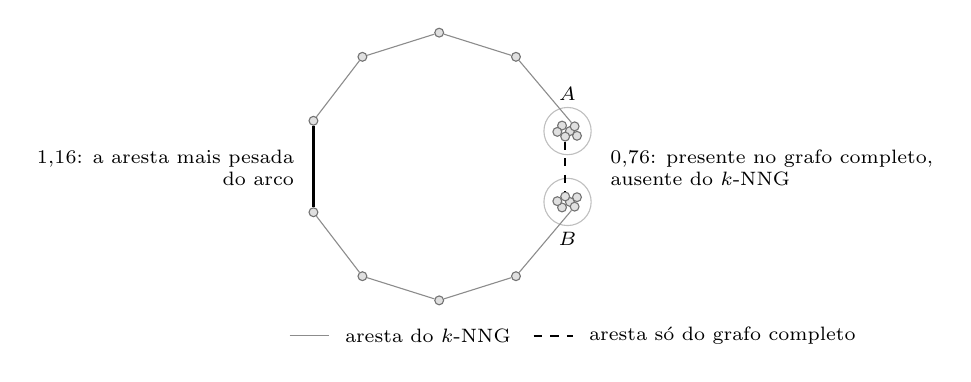
\begin{tikzpicture}[
  pt/.style={circle, draw=black!55, fill=black!12, inner sep=0pt, minimum size=3.2pt},
  knn/.style={black!45, thin},
  heavy/.style={black, thick},
  chord/.style={black, thick, dashed},
  lb/.style={font=\scriptsize}
]
% ---- regiao densa A
\draw[black!25] (1.63,0.45) circle (0.30);
\foreach \x/\y in {1.56/0.52, 1.75/0.39, 1.66/0.45, 1.50/0.44}
  \node[pt] at (\x,\y) {};
\node[pt] (A1) at (1.60,0.38) {};
\node[pt] (A2) at (1.72,0.51) {};
\node[lb] at (1.63,0.92) {$A$};
% ---- regiao densa B
\draw[black!25] (1.63,-0.45) circle (0.30);
\foreach \x/\y in {1.56/-0.52, 1.75/-0.39, 1.66/-0.45, 1.50/-0.44}
  \node[pt] at (\x,\y) {};
\node[pt] (B1) at (1.60,-0.38) {};
\node[pt] (B2) at (1.72,-0.51) {};
\node[lb] at (1.63,-0.92) {$B$};
% ---- arco esparso
\node[pt] (s1) at ( 0.975, 1.393) {};
\node[pt] (s2) at ( 0.000, 1.700) {};
\node[pt] (s3) at (-0.975, 1.393) {};
\node[pt] (s4) at (-1.597, 0.581) {};
\node[pt] (s5) at (-1.597,-0.581) {};
\node[pt] (s6) at (-0.975,-1.393) {};
\node[pt] (s7) at ( 0.000,-1.700) {};
\node[pt] (s8) at ( 0.975,-1.393) {};
\draw[knn] (A2) -- (s1);
\draw[knn] (s1) -- (s2) -- (s3) -- (s4);
\draw[heavy] (s4) -- (s5);
\draw[knn] (s5) -- (s6) -- (s7) -- (s8);
\draw[knn] (s8) -- (B2);
% ---- corda
\draw[chord] (A1) -- (B1);
\node[lb, anchor=west] at (2.05, 0.10) {$0{,}76$: presente no grafo completo,};
\node[lb, anchor=west] at (2.05,-0.15) {ausente do $k$-NNG};
\node[lb, anchor=east] at (-1.72, 0.10) {$1{,}16$: a aresta mais pesada};
\node[lb, anchor=east] at (-1.72,-0.15) {do arco};
% ---- legenda
\draw[knn]   (-1.90,-2.15) -- (-1.40,-2.15);
\node[lb, anchor=west] at (-1.32,-2.15) {aresta do $k$-NNG};
\draw[chord] ( 1.20,-2.15) -- ( 1.70,-2.15);
\node[lb, anchor=west] at ( 1.78,-2.15) {aresta só do grafo completo};
\end{tikzpicture}\\
Fonte: Autoral, sobre a configuração descrita em \cite{core-sg}.
\end{figure}

Esse segundo caso é o que torna a questão empírica em vez de teórica: saber que o \ac{k-NNG} é conexo não basta para concluir que a árvore geradora é dispensável. A Seção \ref{sec:res-connectivity} mede quanto esse resíduo custa em dados reais.\\

% =====================================================================
\section{O problema atacado\label{sec:problems}}
% =====================================================================

\subsection{A construção centralizada e o limite de memória\label{sec:problem-scale}}

O \ac{CORE-SG} resolve o custo de repetir a análise sobre vários valores de $\mpts$, mas sua construção segue um modelo de execução centralizado. Os dois grafos constituintes são calculados e armazenados em um único espaço de memória, sobre o conjunto de dados inteiro, de uma só vez. A \ac{MST} que compõe a segunda metade é, em particular, definida sobre um grafo completo, o que impede que sua construção seja distribuída sem que se materialize ou se percorra $O(n^2)$ pares.\\

Em aceleradores gráficos, essa característica deixa de ser uma questão de tempo e passa a ser uma questão de viabilidade. Há uma assimetria entre os dois recursos que um acelerador oferece. Poder de cálculo é elástico: se a máquina é lenta, espera-se mais, e o resultado eventualmente sai. Memória de dispositivo não é elástica: se a estrutura não cabe, nenhuma quantidade de tempo resolve. A memória de uma \ac{GPU} é tipicamente uma ou duas ordens de grandeza menor que a memória principal de um servidor, é a única memória a que os núcleos do dispositivo têm acesso direto, e essa diferença não tem acompanhado o crescimento do poder de cálculo das próprias \ac{GPU}s.\\

A consequência é um teto abrupto. Uma construção de instância única com $d = 128$ e $\kmax = 32$ ocupa 944 bytes por ponto no dispositivo, o que coloca o limite em torno de $9{,}1 \times 10^6$ pontos em um acelerador de 8 GB. Abaixo desse teto, a construção é rápida; acima dele, ela não executa.\\

O aspecto decisivo é que acrescentar aceleradores ao sistema não move esse teto. Uma construção monolítica não é dividida entre dispositivos: um segundo acelerador não contribui com sua memória, apenas permanece ocioso. O conjunto de dados que não cabe em uma \ac{GPU} continua não cabendo em quatro. Distribuir a construção entre dispositivos só resolve o problema se o método for decomposto de forma que o estado por dispositivo não cresça com o tamanho do conjunto, o que é uma propriedade do projeto do algoritmo e não do hardware.\\

\subsection{Localidade e decomponibilidade\label{sec:incremental-framework}}

A teoria de computação sobre grafos fornece o vocabulário para analisar quando uma estrutura admite esse tipo de decomposição \cite{incremental-computations}. Um problema é dito \textit{limitado} se o custo de atualizá-lo é polinomial nas taxas de mudança da entrada e da saída, o que garante que o custo não dependa do tamanho do grafo. Está demonstrado que consultas fundamentais em grafos são \textit{ilimitadas}, o que impede que computações sobre elas estejam sob esse limite.\\

O mesmo trabalho, entretanto, introduz dois conceitos que conferem eficiência prática mesmo sob operações ilimitadas, e que se aplicam tanto à atualização de uma estrutura quanto à sua construção particionada. O primeiro é o de \textit{computação localizável}: problemas cuja resolução exige apenas a inspeção da vizinhança local de cada elemento, o que delimita o custo pelo tamanho dessa região. O segundo é o de \textit{limitação relativa}: o esforço é comparado ao de reexecutar o algoritmo completo, de modo que a computação se concentre apenas naquilo que de fato importa.\\

A localidade é a propriedade que governa a decomponibilidade. Uma estrutura cuja definição depende apenas de regiões pode ser construída por partes, desde que cada parte contenha a região de que depende; uma estrutura cuja definição é global não pode, porque nenhuma parte contém o que é necessário para decidir. Ambos os conceitos aparecem em algoritmos da literatura sobre grafos dinâmicos. O \ac{MoSSo} \cite{mosso} emprega um agrupamento grosseiro que organiza os vértices por similaridade através de uma variante de \ac{LSH}, reduzindo o espaço de busca de candidatos à fusão, e recorre ao \ac{MCMC} para amostrar uniformemente as vizinhanças dos vértices escolhidos, evitando explorá-las por completo. O \ac{DPGS} \cite{dpgs} também agrupa vértices por similaridade através de \ac{LSH}, sob a hipótese de que vértices próximos são mais propensos a minimizar sua função objetivo, baseada em \ac{MDL}. O IncBoost \cite{inc-boost}, por sua vez, identifica os vértices afetados por cada nova conexão, aplica a eles uma função de vértice e propaga essa aplicação aos vizinhos apenas quando necessário, mantendo uma fronteira de vértices a processar na iteração seguinte.\\

\subsection{A assimetria entre os dois grafos constituintes\label{sec:asymmetry}}

A observação que organiza todo este trabalho é que os dois grafos constituintes do \ac{CORE-SG} se comportam de maneira oposta sob essa taxonomia.\\

O \ac{k-NNG} é localizável. Sua construção depende exclusivamente das vizinhanças de cada vértice, de modo que a lista de vizinhos de um ponto é determinada pelos pontos geometricamente próximos a ele, e não pelo conjunto inteiro. A Figura \ref{fig:knng-increment-reaction} ilustra esse comportamento no caso de um ponto acrescentado a um grafo existente: alguns vértices em torno dele o integram à sua vizinhança, mesmo quando eles próprios não fazem parte da vizinhança do vértice novo, enquanto vértices mais distantes mantêm suas vizinhanças intactas. O \ac{k-NNG} encapsula as localidades do conjunto de dados, e isso é o que torna sua construção decomponível: um bloco de pontos contém, para a maioria de seus membros, boa parte da informação de que suas listas de vizinhança precisam.\\

\begin{figure}[htb!]
\centering
\caption{\label{fig:knng-increment-reaction} Comportamento do incremento no \ac{k-NNG}, arestas coincidentes foram representadas como uma só.}
\includegraphics[width=\textwidth]{cap_materias_e_metodos/knng_increment_reaction.eps}
Fonte: Autoral.
\end{figure}

A \ac{MST} não é localizável. Ela é uma estrutura inerentemente global: a decisão de incluir ou não uma aresta depende de quais partições do grafo ela conecta, e isso é uma propriedade de todo o grafo, não de uma região dele. Nenhum bloco de pontos contém a informação necessária para decidir quais de suas arestas pertencem à árvore do conjunto completo.\\

Há, além disso, um agravante específico ao \ac{CORE-SG} que não se aplica ao cálculo de \ac{MST}s em geral. A árvore de que se precisa não é a de um grafo esparso com pesos fixos, mas a de um grafo \textit{completo} cujos $O(n^2)$ pesos são todos função de $\mpts$, e portanto se deslocam quando o parâmetro muda. Calcular ou manter uma árvore sobre um grafo que nunca é materializado, e cujos pesos dependem de um parâmetro que o usuário varia livremente, é um problema substancialmente mais difícil que o problema clássico.\\

A Figura \ref{fig:knng-is-enough} ilustra a fronteira entre os dois casos. Se muitos vértices próximos entre si estiverem agrupados longe do restante do conjunto, as arestas do \ac{k-NNG} são insuficientes até mesmo para conectar os componentes, e uma aresta que alcance além da $k$-vizinhança é necessária. Em casos menos extremos, porém, os $k$ vizinhos mais próximos de um vértice, por serem os mais próximos, correspondem às arestas de menor peso incidentes a ele, que é exatamente o material de que uma \ac{MST} é feita.\\

\begin{figure}[htb!]
\centering
\caption{\label{fig:knng-is-enough} Como o \ac{k-NNG} pode auxiliar em estimar arestas para a \ac{MST}.}
\includegraphics[width=\textwidth]{cap_materias_e_metodos/knng_is_enough.eps}
Fonte: Autoral.
\end{figure}

Essa assimetria determina o desenho do método. O \ac{k-NNG}, por ser localizável, é decomposto; a \ac{MST}, por ser global, não é decomposta, mas substituída.\\

\subsection{O que o particionamento custa\label{sec:problem-partition-cost}}

A decomponibilidade do \ac{k-NNG} é parcial, e reconhecer o ponto exato em que ela falha é o que delimita a contribuição deste trabalho.\\

Construir um grafo de vizinhança sobre um conjunto particionado significa comparar apenas os pares cujos dois pontos caiam na mesma parte. Todo par cujos pontos estejam separados pela partição permanece não comparado, e se esse par pertencia à vizinhança verdadeira de algum dos dois, a aresta correspondente não aparece no grafo resultante. O grafo produzido por uma construção particionada é, portanto, uma aproximação estritamente pior do que a produzida por uma construção não particionada sobre os mesmos dados e com o mesmo orçamento de iterações.\\

Esse déficit não é um detalhe de implementação, e sim a consequência inevitável de ter dividido o problema. Qualquer método que decomponha a construção de um grafo de vizinhança enfrenta a mesma questão, e as respostas possíveis são três: aceitar a perda, recuperá-la por um passo posterior sobre o grafo mesclado, ou reduzi-la fazendo com que as partes se sobreponham. Este trabalho emprega as duas últimas, e o Capítulo \ref{cha:results} mede o que cada uma custa.\\

Há uma tensão adicional entre as duas. O passo de recuperação opera sobre o grafo mesclado, que é uma estrutura global e, portanto, não decomponível pelo mesmo argumento da Seção \ref{sec:asymmetry}: ele executa na \ac{CPU}, não nos aceleradores. Reduzir o déficit por sobreposição, ao contrário, aumenta o trabalho das instâncias, que executam nos dispositivos. Existe, assim, um parâmetro que desloca trabalho entre os dois lados do sistema, e a identificação desse compromisso é um dos resultados deste trabalho.\\

\subsection{Dados dinâmicos: um problema adjacente\label{sec:problem-dynamic}}

O \ac{CORE-SG} foi concebido no contexto de dados estáticos, e a chegada de novos objetos invalida ambas as estruturas: um objeto novo pode entrar na vizinhança de objetos já existentes, alterando suas listas de vizinhos e, por consequência, suas \textit{core distances}. Na ausência de um mecanismo de atualização, a única resposta possível é reconstruir, o que é caro em termos absolutos e desproporcional à mudança ocorrida.\\

Esse problema é real e foi objeto de investigação ao longo deste projeto. O contexto atual da análise de dados o torna relevante: a quantidade massiva de dados gerados demanda capacidade computacional elevada e levanta discussões sobre eficiência de dados \cite{big-data}, e a geração praticamente ininterrupta produz bases em constante atualização, deslocando o problema do processamento em lote único para o processamento contínuo \cite{data-stream}. Nesse regime, os dados estão ainda sujeitos ao desvio de conceito, em que a adição constante de informação altera a distribuição dos grupos existentes ou cria anomalias que podem ou não vir a se tornar novos grupos \cite{data-stream}.\\

Ele não é, contudo, o problema deste texto. A decisão de delimitar o escopo à construção sobre conjunto fixo foi tomada ao longo da pesquisa, por duas razões. A primeira é que o limite de memória por dispositivo é logicamente anterior: um método que não consegue construir a estrutura inicial não tem o que atualizar. A segunda é que a abstração desenvolvida para resolver o primeiro problema se aplica ao segundo sem modificação estrutural --- uma instância cujo contexto é extraído de um grafo existente estende esse grafo em vez de construí-lo --- de modo que resolver a construção é também estabelecer a base sobre a qual a extensão se apoiaria. Os resultados preliminares obtidos nessa direção são apresentados na Seção \ref{sec:fut-streams}.\\

% =====================================================================
\section{Caminhos investigados e descartados\label{sec:discarded}}
% =====================================================================

Esta seção registra as abordagens que foram estudadas ao longo da pesquisa e posteriormente descartadas ou substituídas. Ela cobre, em particular, a mudança de metodologia ocorrida entre a monografia de qualificação deste mestrado e o trabalho aqui apresentado. A qualificação propunha uma manutenção incremental exata das duas estruturas, acompanhada de uma sumarização localizada do grafo para conter seu crescimento em memória. Durante a fase de pesquisa, verificou-se que ambas as linhas ou eram inviáveis dentro do escopo, ou resolviam um problema mais difícil do que o necessário, e o esforço foi deslocado para as soluções descritas na Seção \ref{sec:adopted}. O registro dessas decisões é parte do resultado da pesquisa, e não uma descrição de trabalho perdido: cada descarte foi motivado por uma constatação específica, e várias delas informaram diretamente o desenho final.

\subsection{Manutenção incremental da MST\label{sec:discarded-mst}}

A primeira linha investigada foi a manutenção exata da \ac{MST} sob inserção. O esquema estudado na qualificação, ilustrado na Figura \ref{fig:mst-edge-case}, era o seguinte: as arestas correspondentes aos $k$ vizinhos mais próximos do vértice novo, já disponíveis pela atualização do \ac{k-NNG}, seriam adicionadas à árvore; o algoritmo de Kruskal \cite{kruskal} seria então executado sobre o conjunto resultante, ordenando as arestas de forma crescente e usando uma estrutura de conjuntos disjuntos \cite{disjoint-sets} para detectar e descartar as que formassem ciclos. A escolha do Kruskal se justificava por sua complexidade depender exclusivamente da quantidade de arestas, e a de conjuntos disjuntos por seu tempo de operação amortizado praticamente constante.\\

\begin{figure}[htb!]
\centering
\caption{\label{fig:mst-edge-case} Comportamento do incremento na \ac{MST}. A adição de um vértice pode formar um caminho que liga dois segmentos da árvore, criando um ciclo que precisa ser desfeito pela remoção da aresta de maior peso.}
\includegraphics[width=\textwidth]{cap_materias_e_metodos/mst_edge_case.eps}
Fonte: Autoral.
\end{figure}

Três constatações levaram ao abandono dessa linha.\\

A primeira é a apontada na Seção \ref{sec:asymmetry}. O objeto a ser mantido não é a \ac{MST} de um grafo esparso, mas a de um grafo completo cujos pesos são função de $\mpts$. A literatura de manutenção dinâmica de \ac{MST} \cite{mst_maintenance} trata do caso em que o grafo subjacente é dado e esparso, e mesmo nesse caso os custos por operação são substanciais. Nenhum dos resultados encontrados se transporta para o caso de um grafo completo implícito com pesos parametrizados, e adaptá-los constituiria, por si só, uma linha de pesquisa independente.\\

A segunda é que o esquema de reexecução do Kruskal a cada lote não é, de fato, incremental no sentido exigido. Ordenar as arestas da árvore existente junto com as novas custa $\Theta(n \log n)$ por lote, o que é assintoticamente melhor que a reconstrução quadrática mas continua sendo função de $n$ e não do tamanho do lote.\\

A terceira, e a decisiva, é que a manutenção exata da árvore resolve um problema mais difícil que o necessário. Como a Seção \ref{sec:coresg-why} estabelece, as únicas arestas que a \ac{MST} contribui ao \ac{CORE-SG} e que o \ac{k-NNG} não fornece são as que ligam componentes separados. Manter a árvore inteira para obter esse subconjunto significa calcular e conservar uma estrutura global cuja quase totalidade é descartada na união. Essa constatação é a origem direta da solução adotada, e vale igualmente para a construção sobre conjunto fixo: o argumento não depende de os dados chegarem ao longo do tempo.\\

\subsection{Manutenção incremental da conectividade\label{sec:discarded-connectivity}}

Uma variante mais modesta da mesma ideia também foi implementada e medida: manter incrementalmente apenas a rotulação de componentes conexos do \ac{k-NNG}, em vez da árvore completa. A estrutura foi construída, é exata, e foi verificada por um certificado que confirma que toda aresta destruída ainda tem seus extremos conectados por algum outro caminho.\\

O resultado foi negativo e é registrado como tal. A manutenção incremental perde para uma recomputação paralela da rotulação por uma margem larga, porque o NN-Descent destrói centenas de milhares de arestas não direcionadas por rodada, e cada destruição exige uma busca bidirecional para verificar se a conectividade foi preservada. A recomputação completa, por outro lado, é uma passagem de união-busca sobre arranjos contíguos de adjacência, que se paraleliza trivialmente e custa poucos milissegundos. O ganho que inicialmente se atribuiu à incrementalidade veio, na verdade, de eliminar a materialização da lista de arestas na recomputação, e não da incrementalidade em si. A funcionalidade permanece implementada e desativada por padrão.\\

\subsection{Sumarização localizada do grafo\label{sec:discarded-summarization}}

A segunda linha proposta na qualificação era a sumarização do \ac{CORE-SG}, como resposta ao crescimento indefinido da estrutura. A sumarização de grafos consiste em descobrir uma representação condensada do grafo, reduzindo a quantidade de vértices e arestas e substituindo-os por supervértices que representam regiões e superarestas que as conectam, minimizando a perda de propriedades relevantes \cite{graph-summarization-survey}. A Figura \ref{fig:summarization-techniques} resume as três técnicas principais identificadas pela literatura: agregação de vértices ou arestas, seleção de subconjuntos ou dispersão da estrutura, e transformação para uma representação de menor dimensionalidade.\\

\begin{figure}[htb!]
\centering
\caption{\label{fig:summarization-techniques} Principais técnicas de sumarização de grafos.}
\includegraphics[width=\textwidth]{cap_referencial_teorico/summarization_techniques.eps}
Fonte: Autoral para (a) e (b); e \cite{network-transformation} para (c).
\end{figure}

A proposta original distinguia-se da literatura por não sumarizar o grafo inteiro. Em vez disso, ao atingir um limiar de memória, os grupos mais densamente relevantes seriam identificados por \ac{FOSC} \cite{fosc} e sumarizados localmente, sob a hipótese de que regiões densas comportam maior compressão com menor perda de informação, pois quanto mais densa uma aglomeração, menos pontos são necessários para representá-la. Dentro de cada grupo, a fusão de pares de vértices seria decidida por um procedimento \ac{MCMC} no estilo Metropolis-Hastings \cite{mcmc}, inspirado no \ac{MoSSo} \cite{mosso}, com uma função custo baseada na variação da entropia de Shannon da distribuição de graus do subgrafo \cite{entropy}. A Figura \ref{fig:knng-summarization} e a Figura \ref{fig:summarization-effect} ilustram o efeito estrutural pretendido sobre o \ac{k-NNG} e sobre a \ac{MST}, respectivamente, e a Figura \ref{fig:summarization-flowchart} descreve o fluxo do procedimento.\\

\begin{figure}[htb!]
\centering
\caption{\label{fig:knng-summarization} Alteração da $k$-vizinhança de um vértice frente à sumarização.}
\includegraphics[width=\textwidth]{cap_referencial_teorico/knng_summarization.eps}
Fonte: Autoral.
\end{figure}

\begin{figure}[htb!]
\centering
\caption{\label{fig:summarization-effect} Como a fusão de vértices altera o \ac{k-NNG} e a \ac{MST} para $\mpts = k = 3$. Em verde os vértices a serem fundidos, em vermelho a superaresta resultante da fusão de arestas conflitantes.}
\includegraphics[width=\textwidth]{cap_materias_e_metodos/summarization_effect.eps}
Fonte: Autoral.
\end{figure}

\begin{figure}[htb!]
\centering
\caption{\label{fig:summarization-flowchart} Fluxograma da sumarização proposta na qualificação.}
\includegraphics[width=\textwidth]{cap_materias_e_metodos/summarization_flowchart.eps}
Fonte: Autoral.
\end{figure}

Quatro razões motivaram a substituição dessa linha.\\

A primeira, e a mais importante, é que o problema que a sumarização resolvia foi resolvido de outra forma. A motivação declarada era conter o consumo de memória. A decomposição em instâncias autocontidas, descrita na Seção \ref{sec:adopted}, limita a memória por dispositivo ao tamanho da instância, que por sua vez é determinado por um parâmetro sob controle do usuário. O consumo por dispositivo passa a ser invariante em relação a $n$ sem que nenhum ponto precise ser descartado ou fundido. Uma técnica com perda deixa de ser necessária quando existe uma sem perda que atinge o mesmo objetivo.\\

A segunda é que a sumarização introduz uma segunda fonte de erro que não é separável da primeira. O objetivo da pesquisa é avaliar quanto a decomposição degrada o resultado em relação a uma referência exata. Se o grafo também for sumarizado, o erro medido passa a ser a soma de duas aproximações independentes, e nenhum experimento consegue atribuir a cada uma sua parcela. Manter o método no nível dos pontos individuais preserva a possibilidade de comparação direta com o objeto exato.\\

A terceira é que a sumarização muda a granularidade da saída, o que compromete a comparabilidade com a literatura. Métodos que agrupam sobre sumários, como Data Bubbles \cite{databubbles}, BIRCH \cite{birch} e seu sucessor numericamente estável BETULA \cite{betula}, ou como o esquema \textit{online-offline} baseado em Bubble-tree \cite{bubble-tree}, produzem partições de microgrupos e não de objetos. Compará-los a uma referência no nível dos pontos confunde o erro introduzido pela sumarização com o erro introduzido pelo método sob avaliação. Ao permanecer no nível dos pontos, este trabalho pode usar como referência o \ac{CORE-SG} exato calculado sobre os mesmos pontos, que é a única referência que ambos os lados de uma comparação podem compartilhar.\\

A quarta é de escopo. Sumarizar uma estrutura exige que a fusão de vértices preserve as propriedades do \ac{k-NNG} e da \ac{MST}, o que, como a Figura \ref{fig:summarization-effect} indica, exige regras próprias de reconstrução estrutural para cada tipo de conflito. Isso excedia o que era realizável no prazo do mestrado com o rigor experimental pretendido. A sumarização permanece como direção de trabalho futuro, discutida no Capítulo \ref{cha:discussion}.\\

\subsection{Índices métricos como estrutura auxiliar\label{sec:discarded-index}}

A qualificação previa o uso do \ac{HNSW} \cite{hnsw} como mecanismo de busca dos $k$ vizinhos mais próximos de cada ponto. O \ac{HNSW} organiza os objetos em um grafo multicamadas, em que a camada base contém todos os objetos e as camadas superiores contêm subconjuntos progressivamente menores, e cada camada é um grafo \ac{NSW} navegável. A busca ocorre de cima para baixo, avançando gulosamente para o vizinho mais próximo do alvo em cada camada e refinando o resultado ao descer.\\

Outras famílias de índices foram consideradas na mesma etapa, incluindo árvores métricas como a M-tree \cite{mtree}, a SS-tree \cite{sstree} e o D-Index \cite{dindex}, estruturas espaciais como a VoR-tree \cite{vortree}, índices de vizinhança reversa como a Rdnn-tree \cite{rdnntree}, e variantes paralelas e dinâmicas em lote como a BDL-tree \cite{bdl-tree}. A literatura de indexação de espaços métricos \cite{metric-indexing} documenta o padrão que motivou o descarte dessa família como estrutura central: métodos exatos de busca por similaridade degradam-se rapidamente em alta dimensionalidade ou sob distribuições não uniformes, a ponto de se tornarem indistinguíveis de uma busca exaustiva \cite{nearest-neighbor-book}.\\

Sob o escopo de construção, o descarte é mais direto do que era sob o escopo de fluxos. Um índice auxiliar existe para localizar rapidamente a vizinhança aproximada de um ponto consultado, o que é exatamente a operação de que uma inserção precisa. A construção sobre conjunto fixo não realiza consultas: todos os pontos estão disponíveis desde o início, e o NN-Descent os processa em bloco, sem que nenhum deles precise ser localizado dentro de uma estrutura preexistente. Manter um segundo índice de vizinhança sobre os mesmos dados acrescentaria custo de memória --- o recurso exatamente sob disputa --- sem oferecer contrapartida. O mecanismo de busca em feixe permanece implementado e é utilizado pelo caminho de extensão descrito na Seção \ref{sec:fut-streams}, onde há de fato consultas a realizar.\\

\subsection{Métricas de similaridade estrutural\label{sec:discarded-metrics}}

A qualificação previa avaliar a fidelidade do grafo resultante por duas métricas estruturais: a média das aproximações dos caminhos mais curtos entre todos os pares de vértices, calculada por um algoritmo de \ac{APSP} aproximado \cite{apsp}, para a conectividade global, e a similaridade de Jaccard entre as vizinhanças originais e resultantes de cada vértice \cite{jaccard}, para a conectividade local.\\

Essas métricas foram substituídas porque respondiam à pergunta errada para o método que se consolidou. Elas medem quanto um grafo sumarizado se parece com o grafo original enquanto grafo, o que é a pergunta adequada quando a saída do método é uma representação condensada da estrutura. A saída deste trabalho não é essa. O objeto que o método existe para produzir é a $\mathrm{MST}_{\mpts}$, e por meio dela a hierarquia de densidade e o agrupamento plano. Duas árvores geradoras podem diferir substancialmente em quais arestas contêm e ainda assim induzir hierarquias praticamente idênticas, porque todas as \ac{MST}s de um grafo compartilham o mesmo multiconjunto de pesos. Medir semelhança estrutural aresta a aresta mediria, nesse caso, o critério de desempate do algoritmo de árvore geradora, e não a qualidade da aproximação. As métricas adotadas em seu lugar, descritas na Seção \ref{sec:metrics}, medem diretamente o objeto de interesse.\\

\subsection{Estratégias de redução do passo de reparo\label{sec:discarded-repair}}

O passo de reparo introduzido pelo particionamento, descrito na Seção \ref{sec:problem-partition-cost}, revelou-se a fase dominante da construção em escala, e por isso recebeu atenção específica. Quatro estratégias de redução foram implementadas e medidas, e nenhuma delas reduziu seu custo a qualidade constante. O registro é feito aqui porque o conjunto dessas tentativas delimita onde o trabalho futuro deve ser dirigido; os números correspondentes estão na Seção \ref{sec:res-repair}.\\

A primeira foi simplesmente encurtar o passo, reduzindo o número de rodadas de refinamento permitidas. A relação entre rodadas e revocação não é gradual: o passo não tolera encurtamento porque as primeiras rodadas estabelecem as vizinhanças das quais as rodadas seguintes dependem.\\

A segunda foi restringir o passo aos vértices que a mesclagem efetivamente alterou, na expectativa de que fossem uma fração pequena. A expectativa não se confirma, e a razão é estrutural: uma construção parte de um grafo vazio, de modo que toda aresta aceita na mesclagem é uma inserção, e o conjunto de vértices alterados é o conjunto inteiro. A estratégia é logicamente aplicável apenas a um grafo preexistente, isto é, ao caminho de extensão.\\

A terceira foi executar o próprio reparo como instâncias, sobre blocos crescidos por localidade, de modo que também ele pudesse ser distribuído entre os dispositivos. O obstáculo é geométrico: um grafo de vizinhança em alta dimensionalidade não admite partição cujos blocos tenham fronteiras pequenas, de modo que o fecho necessário para que cada bloco contenha a informação de que depende cresce a um múltiplo de $n$. Omitir esses fechos torna o reparo decomponível, mas ao custo de perda de revocação.\\

A quarta foi a fusão simétrica de \citeonline{knn_merge}, tratada na subseção seguinte.\\

\subsection{A fusão simétrica de grafos de vizinhança\label{sec:discarded-smerge}}

\citeonline{knn_merge} tratam o problema de mesclar grafos de vizinhança e enunciam diretamente o caso de conjunto fixo: dividir os dados em blocos, construir um grafo aproximado para cada bloco em uma máquina distinta, e reduzir os subgrafos por mesclagens sucessivas de pares. Seu algoritmo de fusão simétrica realiza essa redução por três mecanismos combinados: truncar cada lista de vizinhos, preencher as posições liberadas com candidatos sorteados do outro grafo, e descer comparando apenas pares que cruzem a fronteira entre os dois grafos.\\

A proximidade com o problema deste trabalho é grande o bastante para justificar implementar a fusão simétrica no lugar do passo de reparo e medi-la. O resultado, detalhado na Seção \ref{sec:res-repair}, é que a truncagem da varredura de candidatos responde pela totalidade do efeito na configuração de interesse, e que os dois mecanismos restantes não contribuem. A razão é que o preenchimento oferece candidatos a uma lista ordenada em vez de escrevê-los nela, de modo que uma lista permanece majoritariamente composta por vizinhos do próprio bloco; com muitos blocos, os pares internos ao bloco tornam-se uma minoria pequena o bastante para que filtrá-los não economize nada. A derivação original, feita para dois conjuntos, não se transporta para muitos.\\

O que a truncagem oferece isoladamente é uma curva de tempo contra qualidade melhor que a obtida ao encurtar a descida, mas nenhum comprimento de prefixo alcança a revocação da varredura completa. A fusão simétrica permanece implementada e não é o padrão.\\

% =====================================================================
\section{As decisões adotadas\label{sec:adopted}}
% =====================================================================

\subsection{Separar os dois grafos constituintes\label{sec:adopted-separation}}

A decisão central de projeto decorre da Seção \ref{sec:asymmetry}: como o \ac{k-NNG} e a \ac{MST} falham por razões diferentes, eles são tratados como problemas independentes, com soluções independentes. O \ac{k-NNG}, sendo localizável, é decomposto em subproblemas. A \ac{MST}, sendo global e definida sobre um grafo completo com pesos parametrizados, não é calculada: ela é substituída por uma estimativa cujo custo não depende de $n$.\\

Essa separação é o que torna o problema tratável. Uma solução única para as duas estruturas teria de satisfazer simultaneamente as restrições de ambas, e a mais rígida delas, a globalidade da árvore, dominaria o desenho inteiro. Decompor o \ac{k-NNG} não serviria de nada se, ao final, fosse necessário calcular uma árvore geradora sobre um grafo completo em um único espaço de memória.\\

\subsection{Instâncias independentes para o grafo de vizinhança\label{sec:adopted-instances}}

Para o \ac{k-NNG}, o trabalho parte do NN-Descent \cite{nndescent}, que constrói um grafo aproximado de vizinhança a partir do princípio de que um vizinho de um vizinho é provavelmente um vizinho, convergindo em poucas rodadas de junções locais. Sua variante dinâmica \cite{dynamic_nndescent} amostra diretamente sobre o grafo vivo, limita o cache de vizinhos reversos e remove a necessidade de sincronização dentro de uma rodada, o que a torna adequada a execução paralela sem travas. Ambas as formulações operam sobre um grafo inteiro residente em um único espaço de endereçamento, e é exatamente essa propriedade que este trabalho relaxa.\\

A solução adotada decompõe a construção em \textit{instâncias}: subproblemas autocontidos, cada um reunindo um bloco de pontos, uma amostra de sobreposição extraída dos demais blocos, e as listas de vizinhança desses pontos. Uma permutação aleatória do conjunto é cortada em $m$ blocos, e cada bloco dá origem a uma instância. Uma instância é um problema completo de NN-Descent sem referência a estado global, o que produz três consequências. A memória que ela exige é determinada pelo seu próprio tamanho, e não pelo do conjunto de dados, de modo que um grafo maior que a memória de um acelerador é processado elevando-se $m$. As instâncias nunca se comunicam entre si durante a execução, o que permite enfileirá-las em qualquer dispositivo livre sem protocolo de coordenação. E a quantidade de instâncias define a unidade de paralelismo disponível independentemente da quantidade de dispositivos.\\

\subsection{A sobreposição como parâmetro de projeto\label{sec:adopted-overlap}}

A decomposição acima deixa não comparado todo par cujos pontos caiam em blocos distintos, conforme a Seção \ref{sec:problem-partition-cost}. Duas respostas são combinadas.\\

A primeira é um passo de reparo sobre o grafo mesclado, que é uma nova descida de NN-Descent, agora sobre a estrutura completa. Ele recupera os pares perdidos, mas é global por construção e executa na \ac{CPU}.\\

A segunda é a amostra de sobreposição. Cada instância recebe, além do seu bloco, uma fração adicional de pontos sorteados dos demais blocos. Isso dá às instâncias um conjunto de referência compartilhado --- sem ele, dois blocos só concordam através dos pontos que ambos por acaso contenham --- e faz com que parte dos pares que cruzariam fronteiras seja comparada dentro das instâncias, antes da mesclagem.\\

A sobreposição é, portanto, um parâmetro que desloca trabalho do reparo para a fase de instâncias, isto é, da \ac{CPU} para os dispositivos. Ela aumenta a memória que cada instância ocupa, de modo que a escolha conjunta da quantidade de instâncias e da fração de sobreposição determina simultaneamente a residência por dispositivo, a qualidade do grafo e a fração da construção que escala com a quantidade de aceleradores. O Capítulo \ref{cha:results} caracteriza esse espaço.\\

\subsection{Pontes anti-hub para a árvore geradora\label{sec:adopted-bridges}}

Para a \ac{MST}, a decisão é não calculá-la. A justificativa vem da Seção \ref{sec:coresg-why}: as únicas arestas que a árvore contribui e que a vizinhança não fornece são as que ligam componentes separados. Uma aresta desse tipo parte necessariamente da \textit{borda} de um componente, pois um ponto interior sempre tem um vizinho mais próximo na direção do percurso.\\

Estimar bordas por meios geométricos é impraticável além de poucas dimensões. A solução adotada as estima por uma estatística de vizinhança. O ponto de partida é o fenômeno de \textit{hubness}: em alta dimensionalidade, a relação de vizinhança é assimétrica, e alguns pontos aparecem nas listas de vizinhos de muitos outros enquanto outros aparecem em poucas \cite{hubs}. A literatura estuda esse fenômeno majoritariamente como um problema, e a quantidade reversa foi usada para análise de influência \cite{influencesets} e amparada por estruturas de índice dedicadas \cite{rdnntree}.\\

Este trabalho a usa de forma construtiva, e na extremidade oposta da distribuição. Um ponto interior a um componente está dentro da vizinhança de muitos de seus próprios vizinhos; um ponto de borda está dentro da vizinhança de poucos, porque as listas de seus vizinhos apontam para dentro do componente. O grau reverso, normalizado pelo grau reverso médio dos próprios vizinhos do vértice, é portanto um estimador de borda que é invariante à densidade local, o que é necessário quando os dados misturam densidades. Selecionar apenas os vértices de menor pontuação e calcular uma árvore geradora exata sobre esse conjunto pequeno produz as arestas de ponte. O tamanho do conjunto é fixado pela dimensionalidade e pela quantidade de arestas do grafo, não por $n$.\\

\subsection{Por que essa combinação\label{sec:adopted-why}}

As duas decisões se reforçam. A estimativa de pontes elimina a estrutura global que impediria a decomposição, e a decomposição em instâncias fornece a unidade de paralelismo que torna o método multi-GPU. Nenhuma das duas seria suficiente isoladamente: instâncias autocontidas não ajudariam se, ao final, fosse necessário calcular uma árvore geradora sobre um grafo completo, e a estimativa de pontes não resolveria a memória por dispositivo se o \ac{k-NNG} continuasse a exigir uma passagem sobre todos os pontos em um único espaço de endereçamento.\\

Um subproduto dessa combinação é que o índice de \textit{hubness} mantido para selecionar as pontes armazena as vizinhanças reversas, e essas mesmas listas reversas são o que torna o \ac{k-NNG} navegável para busca em feixe. Um grafo de vizinhança direcionado contém vértices que nenhuma lista aponta, e um percurso que siga apenas arestas diretas não consegue sair deles. Essa propriedade não é explorada pela construção, mas é o que torna o caminho de extensão da Seção \ref{sec:fut-streams} possível sem estrutura adicional.\\

% =====================================================================
\section{Trabalhos relacionados\label{sec:related-work}}
% =====================================================================

Esta seção situa o trabalho em quatro eixos: a construção aproximada de grafos de vizinhança, sua decomposição e fusão, o agrupamento baseado em densidade distribuído ou acelerado, e o uso construtivo de estatísticas de \textit{hubness}.\\

\subsection{Construção aproximada de grafos de vizinhança\label{sec:rel-knng}}

A construção exata de um \ac{k-NNG} custa $O(n^2 d)$, o que a inviabiliza em escala, e a literatura converge para soluções aproximadas. O NN-Descent \cite{nndescent} é o representante central da família baseada em refinamento iterativo: partindo de um grafo aleatório, ele repetidamente compara cada vértice aos vizinhos de seus vizinhos, explorando a transitividade aproximada da relação de proximidade, e converge em poucas rodadas sem exigir qualquer índice espacial. Sua independência em relação à métrica e à dimensionalidade é o que o torna adequado ao contexto deste trabalho, em que os dados são de alta dimensionalidade e a métrica pode ser não euclidiana.\\

O Dynamic NN-Descent \cite{dynamic_nndescent} reformula o método para operar diretamente sobre o grafo em construção, eliminando as duas estruturas auxiliares da formulação original e removendo a necessidade de sincronização dentro de uma rodada. O ganho é de memória e de paralelismo, e é essa variante que serve de base à implementação aqui descrita. Revisões recentes da família de métodos baseados em $k$ vizinhos \cite{knn-review} e das dificuldades de sua aplicação em alta dimensionalidade \cite{knn-challenges} documentam o contexto mais amplo em que esses métodos se inserem.\\

A família alternativa é a dos índices navegáveis, cujo representante dominante é o \ac{HNSW} \cite{hnsw}. A diferença de objetivo é relevante: um índice navegável é otimizado para \textit{consultar} a vizinhança de um ponto dado, ao passo que o NN-Descent é otimizado para \textit{construir} as vizinhanças de todos os pontos simultaneamente. Para a construção sobre um conjunto fixo, em que não há consultas a realizar, a segunda formulação é a apropriada.\\

\subsection{Decomposição e fusão de grafos de vizinhança\label{sec:rel-merge}}

O trabalho mais próximo ao deste texto no eixo da decomposição é o de \citeonline{knn_merge}, que trata da fusão de grafos de vizinhança e enuncia explicitamente o caso de conjunto fixo: dividir os dados em blocos, construir um grafo por bloco em máquinas distintas, e reduzir os subgrafos por mesclagens sucessivas. A partição aqui adotada é a mesma. As diferenças são três. Os $m$ subgrafos são mesclados em uma única passagem sobre as listas globais, e não aos pares. Cada instância carrega uma amostra de sobreposição, de modo que os blocos compartilham um conjunto de referência em vez de serem disjuntos. E o objeto em construção é um \ac{CORE-SG}, e não um \ac{k-NNG} isolado, o que acrescenta a metade de árvore geradora ao problema. A fusão simétrica proposta por aqueles autores foi implementada e medida no lugar do passo de reparo, conforme a Seção \ref{sec:discarded-smerge}.\\

\subsection{Agrupamento baseado em densidade distribuído e acelerado\label{sec:rel-distributed}}

No eixo de escalabilidade existem construções distribuídas em lote. O \ac{HDBSCAN*} sobre MapReduce \cite{mrhdbscan} particiona o espaço de dados recursivamente e calcula hierarquias locais que são posteriormente combinadas; a aceleração por indexação espacial \cite{acceleratedhdbscan} reduz o custo da construção da árvore por meio de estruturas de busca; e o esquema híbrido de \ac{CPU} e \ac{GPU} \cite{bpshdbscan} executa o \ac{DBSCAN} na escala de bilhões de pontos, distribuindo o cálculo de vizinhança entre os dois tipos de processador. Na família de picos de densidade, o UP-DPC \cite{up-dpc} obtém escalabilidade por estimativa aproximada de picos e execução paralela.\\

Esses métodos compartilham uma característica que os distingue do presente trabalho: cada um distribui um agrupamento para um único valor do parâmetro de densidade. Nenhum produz uma estrutura que sirva a uma faixa de valores, que é precisamente a propriedade pela qual o \ac{CORE-SG} existe. Distribuir a construção de um \ac{CORE-SG} é, portanto, um problema distinto de distribuir a construção de um agrupamento.\\

Como linha de base de construção em acelerador, a biblioteca NVIDIA cuML \cite{cuml} implementa o \ac{HDBSCAN*} em \ac{GPU}. Ela serve um valor de $\mpts$ por ajuste, de modo que a propriedade de múltiplos $\mpts$ do \ac{CORE-SG} não tem equivalente naquela implementação e é reportada separadamente. A comparação com ela é informativa por ser uma comparação entre implementações em \ac{CUDA} executando no mesmo dispositivo, o que torna o tempo de relógio uma medida com significado.\\

\subsection{Agrupamento incremental e de fluxos\label{sec:rel-streams}}

Embora fora do escopo deste texto, a literatura de manutenção incremental de estruturas de agrupamento baseado em densidade informa o desenho adotado e é o destino natural do trabalho futuro. O FISHDBC \cite{fishdbc} mantém uma estrutura de agrupamento sob inserção, no nível dos pontos individuais, alimentado por arestas candidatas obtidas de um índice \ac{HNSW} \cite{hnsw}, e mantém uma árvore geradora --- o que constitui exatamente a decisão de projeto oposta à adotada aqui. Ele aproxima o \ac{HDBSCAN*} para um único valor de $\mpts$. O I-HASTREAM \cite{ihastream} mantém uma hierarquia sobre microgrupos, portanto em granularidade distinta, assim como as abordagens de sumarização discutidas na Seção \ref{sec:discarded-summarization}. Ambos se inserem no campo mais amplo do agrupamento de fluxos, para o qual existe revisão abrangente na literatura \cite{data-stream}.\\

\subsection{Hubness e vizinhança reversa\label{sec:rel-hubness}}

A assimetria da relação de vizinhança em alta dimensionalidade foi caracterizada por \citeonline{hubs}, que a descrevem como consequência da concentração de distâncias: à medida que a dimensionalidade cresce, alguns pontos tornam-se vizinhos de um número desproporcional de outros. A literatura trata o fenômeno majoritariamente como um problema a ser mitigado, por afetar negativamente classificadores e métodos de busca.\\

A quantidade reversa --- quantos vértices listam um dado vértice como vizinho --- recebeu atenção em contextos distintos. Conjuntos de influência baseados em consultas de vizinhança reversa foram formalizados por \citeonline{influencesets}, e estruturas de índice dedicadas à manutenção dessas consultas sob inserção foram propostas \cite{rdnntree}. O uso que este trabalho faz dessa estatística difere em dois aspectos: o interesse está na extremidade \textit{inferior} da distribuição, isto é, nos pontos que poucos listam, e a quantidade é normalizada localmente pelos próprios vizinhos do vértice, o que a torna comparável entre regiões de densidades distintas. Não encontramos na literatura consultada uso da estatística de \textit{hubness} como estimador de borda de componente.\\

A dimensionalidade intrínseca é o terceiro elemento desse eixo. O estimador de máxima verossimilhança de \citeonline{levina_bickel} obtém a dimensionalidade efetiva de uma vizinhança a partir das razões entre raios de vizinhos sucessivos, e \citeonline{mackay_ghahramani} corrigem seu viés de agregação. A relevância aqui é que o conjunto de vértices abrangido pela estimativa de pontes é dimensionado pela dimensionalidade, e empregar a dimensionalidade ambiente nessa fórmula degenera em espaços de alta dimensionalidade, conforme a Seção \ref{sec:res-dimension}.\\

\subsection{Posicionamento\label{sec:rel-positioning}}

Em síntese, a construção aproximada de grafos de vizinhança é um campo maduro, com métodos robustos e amplamente validados; a decomposição dessa construção em partes independentes foi proposta e estudada; e o agrupamento baseado em densidade distribuído e acelerado conta com diversas realizações. O que não encontramos na literatura é a interseção: a construção, decomposta entre múltiplos aceleradores, de uma estrutura que sirva a uma faixa de valores do parâmetro de densidade. É essa lacuna que este trabalho ocupa, e é por isso que a linha de base interna principal é a construção de instância única sobre os mesmos dados, e não um método concorrente.\\


% ----------------------------------------------------------
% Materiais e Métodos
% ----------------------------------------------------------
% ---
% Capitulo de Materiais e Metodos
% ---

\chapter{Materiais e Métodos\label{cha:methods}}

Este capítulo especifica o método proposto e o protocolo experimental usado para avaliá-lo. A Seção \ref{sec:overview} apresenta a visão geral da construção. A Seção \ref{sec:notation} fixa a notação. As Seções \ref{sec:knn} e \ref{sec:bridges} detalham, respectivamente, a construção decomposta do grafo de vizinhança e a estimativa que substitui a árvore geradora. A Seção \ref{sec:algorithm} reúne o método em pseudocódigo. A Seção \ref{sec:implementation} descreve a implementação e o esquema de execução em múltiplos aceleradores. A Seção \ref{sec:protocol} especifica o protocolo experimental, incluindo as referências exatas contra as quais a qualidade é medida, as métricas, os conjuntos de dados e as linhas de base.

% =====================================================================
\section{Visão geral do método\label{sec:overview}}
% =====================================================================

A Figura \ref{fig:pipeline} descreve o fluxo de uma construção. O conjunto de dados atravessa quatro etapas.\\

Na primeira, os pontos são particionados em $m$ instâncias. Uma permutação aleatória do conjunto é cortada em $m$ blocos, e cada bloco, acrescido de uma amostra de sobreposição sorteada dos demais blocos, forma uma instância. Cada instância é um problema completo de NN-Descent sobre os seus próprios pontos e é executada em qualquer acelerador disponível.\\

Na segunda, as vizinhanças produzidas pelas instâncias são mescladas nas listas globais dos $\kmax$ melhores. Como o particionamento deixa não comparado todo par cujos pontos caiam em blocos distintos, um passo de reparo sobre o grafo mesclado se segue à mesclagem.\\

Na terceira, o índice de \textit{hubness} é calculado e os candidatos a anti-hub são selecionados; a quantidade de candidatos é $\lceil d \ln |E| \rceil$, onde $d$ é a dimensionalidade adotada para o conjunto de dados e $|E|$ é o número de arestas não direcionadas do \ac{k-NNG}.\\

Na quarta, uma árvore geradora é calculada sobre os anti-hubs selecionados, produzindo as arestas de ponte, seguida de uma etapa de reparo de conectividade que liga quaisquer componentes que as pontes tenham deixado separados, de modo que o resultado seja sempre uma árvore geradora e não uma floresta.\\

Concluída a construção, uma consulta pela $\mathrm{MST}_{\mpts}$ repesa a união das arestas do \ac{k-NNG} com as arestas de ponte usando $\mrd^{\mpts}$ e extrai uma árvore geradora de $O(n\kmax)$ arestas.\\

\begin{figure}[htb!]
\centering
\caption{\label{fig:pipeline} O fluxo de uma construção. As instâncias são subproblemas independentes e constituem a unidade de paralelismo. A mesclagem, o passo de reparo e a árvore geradora das pontes são globais; as duas primeiras operam sobre o grafo inteiro e executam na \ac{CPU}, e a terceira opera sobre um conjunto de $\lceil d\ln|E|\rceil$ vértices, muito menor que o conjunto de dados.}
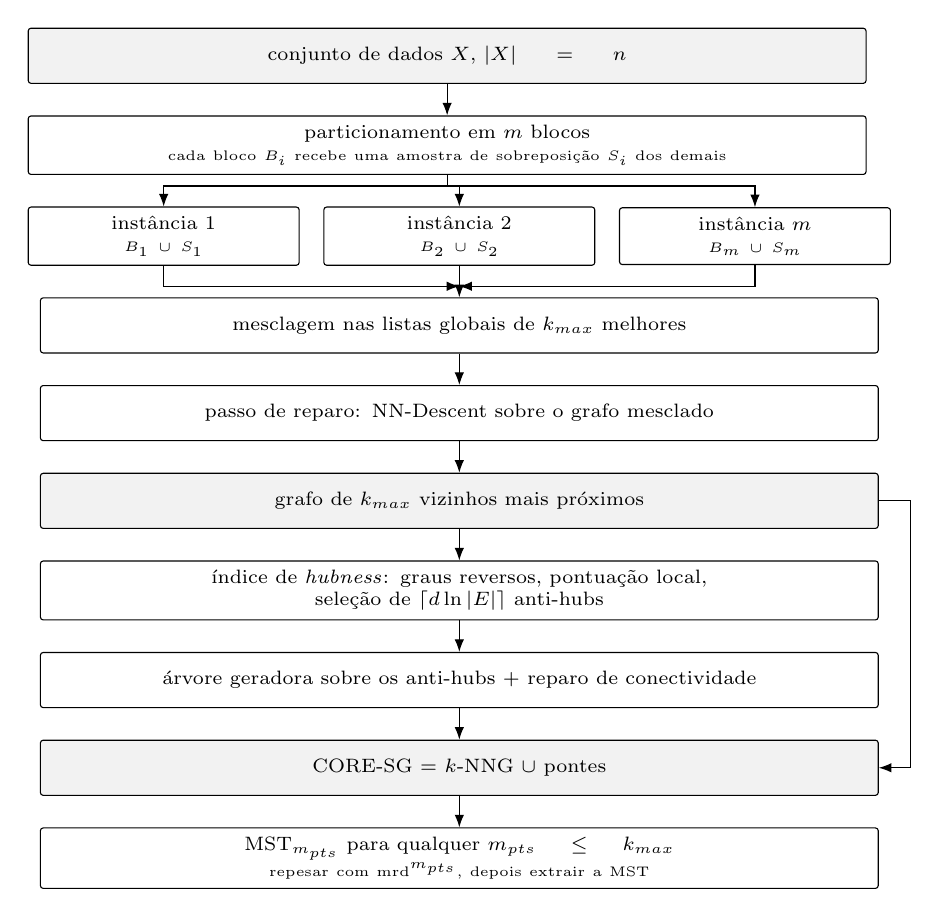
\begin{tikzpicture}[
  node distance=4mm,
  box/.style={draw, rounded corners=1pt, align=center, font=\scriptsize,
              minimum height=7mm, inner xsep=2pt, text width=33mm},
  wide/.style={box, text width=105mm},
  ar/.style={-{Latex[length=1.6mm]}, thin}
]
\node[wide, fill=black!5] (data) {conjunto de dados $X$, $|X| = n$};
\node[wide, below=of data] (part) {particionamento em $m$ blocos\\{\tiny cada bloco $B_i$ recebe uma amostra de sobreposição $S_i$ dos demais}};
\node[box, below=of part.south west, anchor=north west] (i1) {instância 1\\{\tiny $B_1 \cup S_1$}};
\node[box, right=3mm of i1] (i2) {instância 2\\{\tiny $B_2 \cup S_2$}};
\node[box, right=3mm of i2] (i3) {instância $m$\\{\tiny $B_m \cup S_m$}};
\node[wide, below=of i2] (merge) {mesclagem nas listas globais de $\kmax$ melhores};
\node[wide, below=of merge] (refine) {passo de reparo: NN-Descent sobre o grafo mesclado};
\node[wide, below=of refine, fill=black!5] (knn) {grafo de $\kmax$ vizinhos mais próximos};
\node[wide, below=of knn] (hub) {índice de \textit{hubness}: graus reversos, pontuação local,\\seleção de $\lceil d\ln|E|\rceil$ anti-hubs};
\node[wide, below=of hub] (br) {árvore geradora sobre os anti-hubs $+$ reparo de conectividade};
\node[wide, below=of br, fill=black!5] (sg) {CORE-SG $=$ $k$-NNG $\cup$ pontes};
\node[wide, below=of sg] (out) {$\mathrm{MST}_{\mpts}$ para qualquer $\mpts \le \kmax$\\{\tiny repesar com $\mrd^{\mpts}$, depois extrair a MST}};

\draw[ar] (data) -- (part);
\draw[ar] (part.south) -- ++(0,-1.4mm) -| (i1.north);
\draw[ar] (part.south) -- ++(0,-1.4mm) -| (i2.north);
\draw[ar] (part.south) -- ++(0,-1.4mm) -| (i3.north);
\draw[ar] (i1.south) |- ([yshift=1.4mm]merge.north);
\draw[ar] (i2.south) -- (merge.north);
\draw[ar] (i3.south) |- ([yshift=1.4mm]merge.north);
\draw[ar] (merge) -- (refine);
\draw[ar] (refine) -- (knn);
\draw[ar] (knn) -- (hub);
\draw[ar] (hub) -- (br);
\draw[ar] (br) -- (sg);
\draw[ar] (knn.east) -- ++(4mm,0) |- (sg.east);
\draw[ar] (sg) -- (out);
\end{tikzpicture}\\
Fonte: Autoral.
\end{figure}

% =====================================================================
\section{Notação\label{sec:notation}}
% =====================================================================

Seja $X \subset \mathbb{R}^d$ um conjunto de $n$ pontos de dimensionalidade ambiente $d$, e seja $d(\cdot,\cdot)$ uma medida de distância sobre ele. Seguindo a convenção da literatura de agrupamento baseado em densidade, o símbolo $d$ é usado com dois sentidos: isolado, denota a dimensionalidade ambiente, que é um número; acompanhado de dois argumentos, denota a medida de distância. Os dois usos se distinguem sem ambiguidade pela presença dos argumentos.\\

As definições de \textit{core distance} e \textit{mutual reachability distance} são as das equações \eqref{eq:coredist} e \eqref{eq:mrd}. O parâmetro $\kmax$ é o maior valor de $\mpts$ que o grafo deve servir, e $k$ denota o número de vizinhos armazenados por vértice, que neste trabalho é igual a $\kmax$.\\

Denota-se por $m$ a quantidade de instâncias em que a construção é decomposta; por $B_i$ o bloco de pontos da instância $i$; por $\omega$ a fração de sobreposição, isto é, quantos pontos adicionais cada instância recebe em proporção ao seu próprio bloco; por $\mathrm{NN}(v)$ a lista de vizinhos armazenada para o vértice $v$; e por $|E|$ o número de arestas não direcionadas do \ac{k-NNG} resultante.\\

% =====================================================================
\section{O grafo de vizinhança: instâncias independentes\label{sec:knn}}
% =====================================================================

\subsection{A instância\label{sec:instance}}

Uma instância é a unidade de decomposição da construção. Ela reúne um bloco de pontos, uma amostra de sobreposição extraída dos demais blocos, e as listas de vizinhança desses pontos, e constitui um problema completo de NN-Descent sem referência a estado global.\\

A construção parte de uma permutação aleatória de $X$, cortada em $m$ blocos $B_1, \dots, B_m$ de tamanho aproximadamente $n/m$. A permutação é necessária: cortar o conjunto na ordem em que ele é lido produziria blocos correlacionados com a ordem de armazenamento, que em conjuntos reais frequentemente reflete alguma estrutura, e isso tornaria os resultados dependentes de uma propriedade acidental do arquivo.\\

Três consequências decorrem dessa construção, e são elas que respondem ao problema da Seção \ref{sec:problem-scale}. A memória que uma instância exige é determinada pelo seu próprio tamanho, independentemente do tamanho do conjunto de dados, de modo que um grafo maior do que a memória de um acelerador é processado elevando-se $m$. As instâncias não se comunicam entre si durante a execução e podem portanto ser enfileiradas em qualquer dispositivo livre. E a quantidade de instâncias define a unidade de paralelismo disponível, independentemente de quantos dispositivos a executem; manter $m$ maior ou igual à quantidade de dispositivos é o que mantém todos ocupados.\\

\subsection{A sobreposição\label{sec:overlap}}

Blocos disjuntos deixam não comparado todo par cujos dois pontos caiam em blocos distintos, e deixam também as instâncias sem referência comum: dois blocos só concordariam entre si através dos pontos que ambos por acaso contivessem, o que em uma partição disjunta é nenhum.\\

Cada instância recebe, por isso, além do seu bloco $B_i$, uma amostra $S_i$ de $\omega|B_i|$ pontos sorteados uniformemente entre os demais blocos. O tamanho da instância é, portanto,
\begin{equation}
\label{eq:instancesize}
m_i = (1 + \omega)\,\frac{n}{m},
\end{equation}
antes de removidos os sorteios repetidos.\\

A sobreposição tem dois efeitos, e ambos importam. O primeiro é dar às instâncias um conjunto de referência compartilhado, de modo que vizinhanças descobertas em instâncias distintas possam ser confrontadas na mesclagem. O segundo é que parte dos pares que cruzariam fronteiras passa a ser comparada dentro das instâncias, antes da mesclagem, o que reduz o trabalho que resta ao passo de reparo.\\

Esse segundo efeito é o que torna $\omega$ um parâmetro de projeto, acima de um detalhe de implementação. A fase de instâncias executa nos aceleradores; o passo de reparo não. Elevar $\omega$ aumenta a primeira e reduz o segundo, isto é, desloca trabalho da \ac{CPU} para os dispositivos, ao custo de ocupar mais memória por instância. A Seção \ref{sec:res-overlap} caracteriza esse compromisso, e mostra em particular que elevar $m$ e $\omega$ conjuntamente mantém a residência por dispositivo aproximadamente constante enquanto melhora simultaneamente a qualidade e a escalabilidade.\\

\subsection{A restrição de parada\label{sec:constraints}}

A descida dentro de uma instância termina quando uma rodada produz menos de $\delta k m_i$ atualizações, onde $m_i$ é o tamanho da instância. O critério é expresso em função do tamanho da instância, independentemente do conjunto de dados, o que o mantém atrelado ao subproblema: um critério expresso como fração de $n$ faria instâncias pequenas pararem cedo demais ou tarde demais conforme $m$ variasse.\\

\subsection{O custo de memória por dispositivo\label{sec:devicecost}}

O custo por ponto que uma instância impõe ao dispositivo é
\begin{equation}
\label{eq:devicecost}
c = 4\,\mathrm{stride} + 8k + s,
\end{equation}
em que $\mathrm{stride}$ é o comprimento do vetor após alinhamento, $k$ é o tamanho da vizinhança e $s$ é o estado de amostragem do NN-Descent. Uma instância ocupa, portanto, $c\,m_i$ bytes, com $m_i$ dado pela Equação \eqref{eq:instancesize}, e é a maior instância que decide se uma configuração cabe em um dado acelerador.\\

Duas convenções de unidade são usadas ao longo do texto, e a distinção importa porque os limites derivados desta equação dependem dela. As capacidades de dispositivo seguem a rotulação do fabricante, em múltiplos binários, de modo que um acelerador de 8\,GB oferece $2^{33} = 8{,}59 \times 10^9$ bytes. As quantidades medidas e reportadas, como as residências da Seção \ref{sec:res-memory}, estão em múltiplos decimais de $10^6$ e $10^9$ bytes.\\

Essa expressão é a resposta operacional ao problema da Seção \ref{sec:problem-scale}. Dada a memória disponível em um dispositivo, os pares $(m, \omega)$ que cabem nele são calculáveis, e não precisam ser descobertos por tentativa. A Seção \ref{sec:res-memory} reporta a grandeza diretamente medida.\\

\subsection{Mesclagem\label{sec:merge}}

Concluídas as instâncias, suas vizinhanças são mescladas no grafo global por inserção repetida em listas ordenadas dos $\kmax$ melhores: cada instância oferece as vizinhanças que descobriu, e cada candidato é aceito apenas se melhorar a lista em que é oferecido.\\

Essa operação é comutativa e associativa, o que significa que o resultado mesclado não depende da ordem em que as instâncias terminam nem de como seus resultados são agrupados, e é idempotente, o que significa que mesclar a mesma vizinhança duas vezes não altera nada. As instâncias podem, portanto, terminar em qualquer ordem, e o escalonador não precisa de nenhum protocolo de coordenação além de recolher os resultados.\\

Como as instâncias se sobrepõem, um mesmo vértice pode receber contribuições de mais de uma delas, e a mesclagem é o ponto em que essas contribuições são confrontadas. É essa propriedade que faz da sobreposição um mecanismo útil em vez de um desperdício de trabalho duplicado.\\

\subsection{O passo de reparo\label{sec:repair-pass}}

O particionamento deixa não comparado todo par cujos pontos não compartilhem nenhuma instância, de modo que o grafo mesclado omite vizinhos que uma descida única e indivisa teria encontrado. Um passo de reparo, que é uma nova execução de NN-Descent sobre o grafo mesclado, os recupera.\\

Esse passo existe exclusivamente como consequência do particionamento: em $m = 1$ o resultado da descida é adotado diretamente e nenhum reparo é executado. Ele opera sobre o grafo inteiro e é, por isso, global no sentido da Seção \ref{sec:asymmetry}; ele executa na \ac{CPU}, e é a fase que não escala com a quantidade de aceleradores.\\

O passo de reparo é a fase dominante de uma construção em escala, e por isso recebeu atenção específica. Nenhuma das quatro estratégias de redução da Seção \ref{sec:discarded-repair} o encurtou a qualidade constante. O que o reduz é a sobreposição da Seção \ref{sec:overlap}, que não o encurta mas desloca parte de seu trabalho para as instâncias. A Seção \ref{sec:res-repair} reporta as medições correspondentes.\\

% =====================================================================
\section{A árvore geradora: pontes anti-hub\label{sec:bridges}}
% =====================================================================

\subsection{O estimador de borda\label{sec:score}}

Como estabelecido na Seção \ref{sec:adopted-bridges}, a árvore geradora só precisa fornecer arestas que atravessem componentes separados por densidade, e tal ponte parte da borda de um componente. Define-se, para um vértice $v$ do \ac{k-NNG} com conjunto de vizinhos $\mathrm{NN}(v)$,
\begin{equation}
\label{eq:rd}
\mathrm{rd}(v) = \left| \{\, u : v \in \mathrm{NN}(u) \,\} \right|,
\end{equation}
o grau reverso, isto é, o número de vértices que listam $v$ entre seus próprios $k$ vizinhos mais próximos, e
\begin{equation}
\label{eq:score}
\mathrm{score}(v) = \frac{\mathrm{rd}(v)}
     {\dfrac{1}{|\mathrm{NN}(v)|}\displaystyle\sum_{u \in \mathrm{NN}(v)} \mathrm{rd}(u)},
\end{equation}
o grau reverso de $v$ dividido pelo grau reverso médio sobre os próprios vizinhos de $v$.\\

Um ponto interior está dentro de muitas das vizinhanças de seus vizinhos; um ponto de borda está dentro de poucas, porque as listas de seus vizinhos apontam de volta para dentro do componente. O denominador é o que torna \eqref{eq:score} utilizável: comparar $\mathrm{rd}(v)$ contra a população global apenas encontraria os componentes esparsos, ao passo que compará-lo contra a própria vizinhança de $v$ torna a pontuação invariante à densidade local. Um ponto de borda de um componente denso pontua como um ponto de borda de um componente esparso, o que é necessário quando os dados misturam densidades. Valores abaixo de 1 indicam um anti-hub local.\\

A Figura \ref{fig:antihub} ilustra os dois mecanismos. O painel (a) mostra a assimetria que o numerador captura: um vértice interior é apontado por muitos de seus vizinhos, um vértice de borda por poucos. O painel (b) mostra por que o denominador é indispensável. Uma ordenação pelo grau reverso bruto colocaria todos os vértices do componente esparso à frente da borda do componente denso, e o orçamento de seleção seria consumido por um único componente; a normalização local desloca ambas as bordas para valores abaixo de 1 e ambos os interiores para valores próximos de 1, de modo que a ordenação passa a separar bordas de interiores em vez de separar componentes densos de esparsos.\\

\begin{figure}[htb!]
\centering
\caption{\label{fig:antihub} O estimador de borda de \eqref{eq:score}. Em (a), arestas direcionadas do \ac{k-NNG} apontando para um vértice interior $v$ e para um vértice de borda $u$: o interior está na lista de vizinhos de muitos, a borda na de poucos. Em (b), dois componentes de densidades distintas, com o grau reverso $\mathrm{rd}$ e a pontuação de \eqref{eq:score} anotados; o grau reverso bruto ordena por densidade, a pontuação normalizada ordena por posição no componente.}
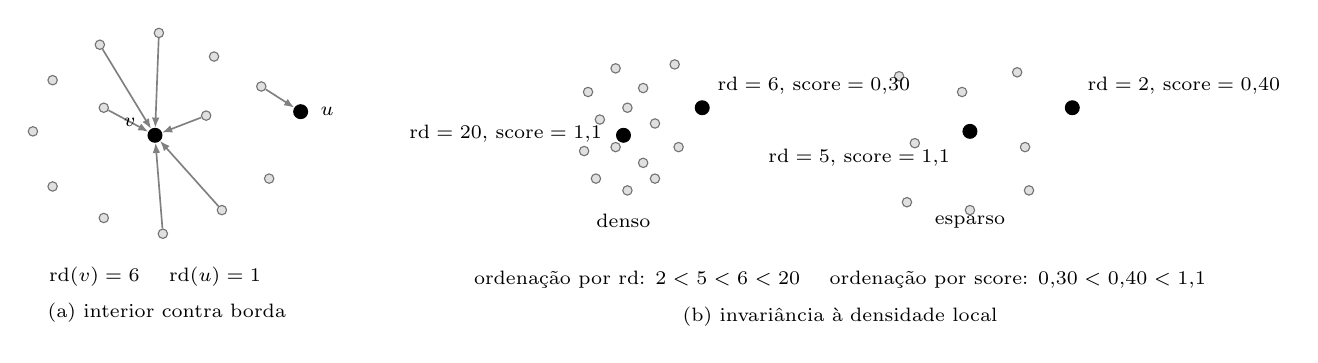
\begin{tikzpicture}[
  pt/.style={circle, draw=black!55, fill=black!12, inner sep=0pt, minimum size=3.4pt},
  hi/.style={circle, draw=black, fill=black, inner sep=0pt, minimum size=5pt},
  ar/.style={-{Latex[length=1.3mm]}, black!50, semithick},
  lb/.style={font=\scriptsize},
  cp/.style={font=\scriptsize}
]
% ---------- painel (a) ----------
\begin{scope}
  \node[pt] (a1)  at (-1.30, 0.70) {};
  \node[pt] (a2)  at (-0.70, 1.15) {};
  \node[pt] (a3)  at ( 0.05, 1.30) {};
  \node[pt] (a4)  at ( 0.75, 1.00) {};
  \node[pt] (a5)  at ( 1.35, 0.62) {};
  \node[pt] (a6)  at (-1.55, 0.05) {};
  \node[pt] (a7)  at (-0.65, 0.35) {};
  \node[hi] (v)   at ( 0.00, 0.00) {};
  \node[pt] (a9)  at ( 0.65, 0.25) {};
  \node[hi] (u)   at ( 1.85, 0.30) {};
  \node[pt] (a11) at (-1.30,-0.65) {};
  \node[pt] (a12) at (-0.65,-1.05) {};
  \node[pt] (a13) at ( 0.10,-1.25) {};
  \node[pt] (a14) at ( 0.85,-0.95) {};
  \node[pt] (a15) at ( 1.45,-0.55) {};
  \foreach \s in {a7,a9,a3,a13,a2,a14} \draw[ar] (\s) -- (v);
  \draw[ar] (a5) -- (u);
  \node[lb, anchor=east] at (-0.12, 0.16) {$v$};
  \node[lb, anchor=west] at ( 1.98, 0.30) {$u$};
  \node[lb, anchor=north] at (0.0,-1.55) {$\mathrm{rd}(v) = 6$ \quad $\mathrm{rd}(u) = 1$};
  \node[cp, anchor=north] at (0.15,-2.00) {(a) interior contra borda};
\end{scope}
% ---------- painel (b) ----------
\begin{scope}[xshift=6.4cm]
  % componente denso
  \foreach \x/\y in {-0.9/0.55, -0.55/0.85, -0.2/0.6, -0.75/0.2, -0.4/0.35,
                     -0.05/0.15, -0.95/-0.2, -0.55/-0.15, -0.2/-0.35,
                     -0.8/-0.55, -0.4/-0.7, -0.05/-0.55, 0.2/0.9, 0.25/-0.15}
     \node[pt] at (\x,\y) {};
  \node[hi] (di) at (-0.45,0.0) {};
  \node[hi] (db) at ( 0.55,0.35) {};
  \node[lb, anchor=south] at (-0.45,-1.30) {denso};
  % componente esparso
  \foreach \x/\y in {3.05/0.75, 3.85/0.55, 4.55/0.8, 3.25/-0.1, 4.65/-0.15,
                     3.15/-0.85, 3.95/-0.95, 4.70/-0.70}
     \node[pt] at (\x,\y) {};
  \node[hi] (si) at (3.95,0.05) {};
  \node[hi] (sb) at (5.25,0.35) {};
  \node[lb, anchor=south] at (3.95,-1.30) {esparso};
  % anotacoes
  \node[lb, anchor=east]       at (-0.60, 0.02) {$\mathrm{rd}=20$, $\mathrm{score}=1{,}1$};
  \node[lb, anchor=south west] at ( 0.62, 0.40) {$\mathrm{rd}=6$, $\mathrm{score}=0{,}30$};
  \node[lb, anchor=north east] at ( 3.82,-0.05) {$\mathrm{rd}=5$, $\mathrm{score}=1{,}1$};
  \node[lb, anchor=south west] at ( 5.32, 0.40) {$\mathrm{rd}=2$, $\mathrm{score}=0{,}40$};
  \node[lb, anchor=north] at (2.3,-1.60)
     {ordenação por $\mathrm{rd}$: $2 < 5 < 6 < 20$ \quad ordenação por $\mathrm{score}$: $0{,}30 < 0{,}40 < 1{,}1$};
  \node[cp, anchor=north] at (2.3,-2.05) {(b) invariância à densidade local};
\end{scope}
\end{tikzpicture}\\
Fonte: Autoral.
\end{figure}

Duas observações sobre a forma de \eqref{eq:score} merecem registro. A média divide por $|\mathrm{NN}(v)|$ em lugar de por $k$, porque um vértice recém-inserido pode ter uma lista mais curta que $k$ antes do refinamento, e dividir por $k$ nesse caso não produziria uma média aritmética. E o limite superior da pontuação não é $k$: conforme os graus dos vizinhos caem, a pontuação cresce sem limite superior, ao passo que seu ponto neutro é 1.\\

\subsection{A seleção\label{sec:selection}}

A estimativa consiste em selecionar os $\lceil d \ln |E| \rceil$ vértices de menor pontuação e calcular uma \ac{MST} exata sobre esse conjunto no espaço de \textit{mutual reachability}. Suas arestas tornam-se as pontes, armazenadas com sua distância métrica original, de modo que o repeso para uma consulta em um dado $\mpts$ as trate de forma idêntica às arestas do \ac{k-NNG}.\\

O tamanho do conjunto selecionado depende de $d$ e de $|E|$, e não de $n$, e a escolha de $|E|$ em vez de $n$ é deliberada. O que as pontes precisam cobrir é o conjunto de lugares que as vizinhanças não alcançam, e isso é uma propriedade de quão ricamente o grafo está conectado, não de quantos pontos ele contém: $n$ pontos com $\kmax = 64$ deixam muito menos lacunas que os mesmos $n$ pontos com $\kmax = 8$. A contagem de arestas carrega essa informação e a contagem de pontos não. Usar $\ln |E|$ em vez de $|E|$ então impede que o termo cresça com o grafo em qualquer sentido prático, já que $|E|$ é ele próprio $O(n\kmax)$ e seu logaritmo se desloca em 0,69 a cada duplicação. O cálculo das pontes é, portanto, $O(m^2 d)$ para $m$ anti-hubs selecionados, com $m \ll n$, e nenhuma árvore geradora precisa ser mantida conforme os pontos chegam.\\

\subsection{Dimensionalidade ambiente e dimensionalidade intrínseca\label{sec:intrinsic}}

O termo $d$ em $\lceil d \ln |E| \rceil$ é, na formulação acima, a dimensionalidade ambiente, isto é, o número de coordenadas que cada ponto carrega. Isso degenera em alta dimensionalidade: quando $d$ é da ordem de centenas ou milhares, o produto $d \ln |E|$ pode exceder o próprio $n$, e a seleção passa a conter todos os pontos, momento em que a estimativa se torna a \ac{MST} exata que ela existe para substituir.\\

A alternativa implementada substitui $d$ por uma dimensionalidade \ac{ID} estimada por máxima verossimilhança a partir dos raios de vizinhança já armazenados \cite{levina_bickel}, agregada entre os pontos pela média harmônica \cite{mackay_ghahramani}, que é o agrupamento não enviesado desse estimador e o único robusto a estimativas locais explodidas. O estimador é gratuito no sentido de que consome apenas as distâncias que o \ac{k-NNG} já contém, ao custo de $O(n k)$. Um limitador adicional, expresso sobre o custo em operações de par em lugar da contagem de anti-hubs, limita o custo quando o estimador de dimensionalidade não é confiável. A Seção \ref{sec:res-sensitivity} apresenta a comparação medida entre as duas regras.\\

\subsection{Cota por componente\label{sec:quota}}

A pontuação de \eqref{eq:score} ordena vértices dentro da região em que eles se situam, o que é o que a torna utilizável entre componentes de densidades diferentes. Ordenar é, contudo, uma operação global, e a contagem $\lceil d \ln |E| \rceil$ é função da dimensionalidade e da contagem de arestas, de modo que a seleção não tem conhecimento de quantos componentes o grafo possui. Onde os componentes superam essa contagem, ou quase a superam, alguns deles não contribuem nenhum vértice selecionado e nenhuma ponte pode partir deles.\\

Uma cota por componente fecha essa lacuna ao garantir a todo componente do \ac{k-NNG} um número mínimo fixo de posições na seleção, preenchidas por seus próprios vértices de menor pontuação, além daquelas que a ordenação global escolhe. Os dois mecanismos operam em conjunto: a ordenação seleciona, dentro de um componente, os vértices adequados para servir de origem a uma ponte, e a cota garante que cada componente tenha ao menos um vértice selecionado.\\

A cota cobre ainda um caso que a ordenação não alcança sozinha. Em um componente pequeno, destacado e de densidade uniforme, todo vértice tem o mesmo grau reverso de seus vizinhos, de modo que todos pontuam exatamente 1 e nenhum é um anti-hub segundo a ordenação, por mais isolado que o componente esteja. Selecionar por componente ainda assim escolhe os vértices mais periféricos daquele componente, porque a cota é preenchida a partir da ordem de pontuação interna a ele.\\

\subsection{Reparo de conectividade\label{sec:repair}}

A seleção é uma estimativa, de modo que as pontes que ela produz podem ainda deixar dois componentes sem ligação, e uma estrutura geradora que não é conexa é uma floresta e não uma árvore. A etapa de reparo liga o que restou. Ela calcula uma árvore geradora sobre um conjunto de representantes extraídos de cada componente sobrevivente, e depois mantém apenas as arestas cujos extremos estão em componentes diferentes. Esse subconjunto basta para conectar tudo: contrair cada componente a um único vértice transforma a árvore de representantes em um grafo conexo sobre os componentes, e as arestas que sobrevivem ao filtro são exatamente aquelas de que esse grafo é feito. A Figura \ref{fig:repair} ilustra o procedimento com três componentes remanescentes e dois representantes por componente.\\

\begin{figure}[htb!]
\centering
\caption{\label{fig:repair} A etapa de reparo. Após as pontes, restam três componentes. Uma árvore geradora é calculada sobre os seis representantes, produzindo cinco arestas; as três cujos extremos caem no mesmo componente são descartadas, e as duas restantes bastam para conectar os três componentes, que é exatamente o número de arestas de uma árvore geradora sobre três vértices.}
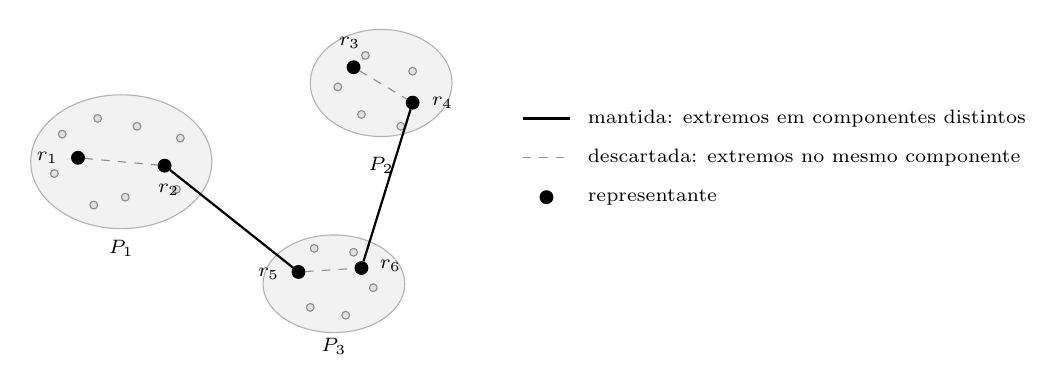
\begin{tikzpicture}[
  blob/.style={draw=black!30, fill=black!5},
  pt/.style={circle, draw=black!45, fill=black!12, inner sep=0pt, minimum size=2.8pt},
  rep/.style={circle, draw=black, fill=black, inner sep=0pt, minimum size=4.6pt},
  keep/.style={black, thick},
  drop/.style={black!45, dashed, thin},
  lb/.style={font=\scriptsize},
  cp/.style={font=\scriptsize}
]
% componentes
\draw[blob] (0,0) ellipse (1.15 and 0.85);
\draw[blob] (3.30,1.00) ellipse (0.90 and 0.68);
\draw[blob] (2.70,-1.55) ellipse (0.90 and 0.62);
\node[lb] at (0,-1.10) {$P_1$};
\node[lb] at (3.30,-0.05) {$P_2$};
\node[lb] at (2.70,-2.35) {$P_3$};
% pontos internos
\foreach \x/\y in {-0.75/0.35, -0.30/0.55, 0.20/0.45, 0.75/0.30, -0.85/-0.15,
                   0.05/-0.45, 0.70/-0.35, -0.35/-0.55}
   \node[pt] at (\x,\y) {};
\foreach \x/\y in {3.05/0.60, 3.55/0.45, 3.70/1.15, 3.10/1.35, 2.75/0.95}
   \node[pt] at (\x,\y) {};
\foreach \x/\y in {2.45/-1.10, 2.95/-1.15, 3.20/-1.60, 2.40/-1.85, 2.85/-1.95}
   \node[pt] at (\x,\y) {};
% representantes
\node[rep] (r1) at (-0.55, 0.05) {};
\node[rep] (r2) at ( 0.55,-0.05) {};
\node[rep] (r3) at ( 2.95, 1.20) {};
\node[rep] (r4) at ( 3.70, 0.75) {};
\node[rep] (r5) at ( 2.25,-1.40) {};
\node[rep] (r6) at ( 3.05,-1.35) {};
\node[lb, anchor=east]  at (-0.68, 0.05) {$r_1$};
\node[lb, anchor=north] at ( 0.60,-0.16) {$r_2$};
\node[lb, anchor=south] at ( 2.90, 1.32) {$r_3$};
\node[lb, anchor=west]  at ( 3.82, 0.75) {$r_4$};
\node[lb, anchor=east]  at ( 2.13,-1.42) {$r_5$};
\node[lb, anchor=west]  at ( 3.16,-1.32) {$r_6$};
% arvore geradora sobre os representantes
\draw[drop] (r1) -- (r2);
\draw[drop] (r3) -- (r4);
\draw[drop] (r5) -- (r6);
\draw[keep] (r2) -- (r5);
\draw[keep] (r6) -- (r4);
% legenda
\draw[keep] (5.10,0.55) -- (5.70,0.55);
\node[lb, anchor=west] at (5.80,0.55) {mantida: extremos em componentes distintos};
\draw[drop] (5.10,0.05) -- (5.70,0.05);
\node[lb, anchor=west] at (5.80,0.05) {descartada: extremos no mesmo componente};
\node[rep] at (5.40,-0.45) {};
\node[lb, anchor=west] at (5.80,-0.45) {representante};
\end{tikzpicture}\\
Fonte: Autoral.
\end{figure}

Ambos os mecanismos precisam saber a que componente pertence cada vértice, de modo que uma rotulação de componentes é calculada uma vez por atualização. Ela é uma passagem de união-busca sobre os arranjos de adjacência do \ac{k-NNG}, que percorre todos os vértices; adicionar as arestas de ponte à rotulação em seguida custa uma união adicional por ponte. O fato de a rotulação ser global levanta a pergunta óbvia de por que a pontuação anti-hub é necessária, se os componentes são conhecidos de qualquer forma. A resposta é que saber quais vértices pertencem a um componente não diz de qual deles uma ponte deve partir, e um componente pode conter milhões de vértices. Ligar componentes diretamente exigiria uma busca entre todos os pares de dois deles; a pontuação é o que reduz cada componente ao punhado de vértices de borda que vale a pena considerar, e a árvore geradora é então calculada sobre esse conjunto pequeno.\\

\subsection{O índice de hubness como observador\label{sec:hubindex}}

Duas propriedades da implementação merecem ser enunciadas. O índice de \textit{hubness} se acopla ao \ac{k-NNG} como um observador, de modo que toda aresta direcionada inserida ou removida atualiza um grau reverso em $O(1)$ e marca os vértices afetados; uma atualização repontua apenas a região afetada, em vez de todos os $n$ vértices.\\

Além disso, o índice mantém as próprias vizinhanças reversas, além dos graus reversos, o que torna exata a propagação da pontuação após uma atualização. Isso porque $\mathrm{score}(v)$ depende de $\mathrm{rd}(u)$ para $u \in \mathrm{NN}(v)$, de modo que os vértices que precisam ser repontuados quando o grau reverso de um vértice $u$ muda são aqueles que têm $u$ como vizinho, isto é, os vizinhos reversos de $u$. Essas mesmas listas são o que torna o grafo navegável para busca em feixe, propriedade que a construção não utiliza mas da qual o caminho de extensão da Seção \ref{sec:fut-streams} depende. O custo dessa escolha é um inteiro por aresta direcionada, e ela pode ser desativada, momento em que a propagação recai para uma aproximação sobre arestas diretas e a busca segue apenas arestas diretas.\\

% =====================================================================
\section{O algoritmo\label{sec:algorithm}}
% =====================================================================

O método é apresentado em duas rotinas, correspondentes às duas metades do \ac{CORE-SG}. O Algoritmo \ref{alg:knn} constrói o grafo de vizinhança por decomposição em instâncias, cobrindo as duas primeiras etapas da Figura \ref{fig:pipeline}. O Algoritmo \ref{alg:bridges} estima a metade de árvore geradora, cobrindo as duas últimas. As duas rotinas não compartilham estado além do \ac{k-NNG} concluído, o que é a razão de serem descritas e medidas separadamente.\\

A extração da $\mathrm{MST}_{\mpts}$ para um valor específico do parâmetro é a consulta, e não a construção: ela consiste em repesar com $\mrd^{\mpts}$ a união das arestas produzidas pelas duas rotinas e executar um algoritmo de árvore geradora mínima sobre elas.\\

\begin{algorithm}[htb!]
\caption{\label{alg:knn} O grafo de vizinhança, a partir de instâncias independentes}
\begin{algorithmic}[1]
\REQUIRE conjunto $X$ com $|X| = n$; tamanho de vizinhança $\kmax$; quantidade de instâncias $m$; fração de sobreposição $\omega$; taxa de parada $\delta$; rodadas de reparo $r$
\ENSURE grafo $G$ de $\kmax$ vizinhos mais próximos sobre $X$
\STATE corte uma permutação aleatória de $X$ em blocos $B_1, \dots, B_m$
\FOR{$i \leftarrow 1$ \TO $m$}
    \COMMENT{independentes; qualquer acelerador}
    \STATE $S_i \leftarrow \omega|B_i|$ pontos sorteados uniformemente em $X \setminus B_i$
    \STATE $V_i \leftarrow B_i \cup S_i$
    \STATE $H_i \leftarrow \textsc{NNDescent}(V_i, \kmax)$, parando quando uma rodada produzir menos de $\delta\kmax|V_i|$ atualizações
\ENDFOR
\STATE $G \leftarrow$ listas vazias de $\kmax$ melhores sobre $X$
\FOR{$i \leftarrow 1$ \TO $m$}
    \COMMENT{mesclagem; independente da ordem}
    \FORALL{$v \in B_i$ e $(u, w) \in H_i[v]$}
        \STATE ofereça $(u, w)$ a $G[v]$, que retém os $\kmax$ menores
    \ENDFOR
\ENDFOR
\IF{$m > 1$}
    \STATE $G \leftarrow \textsc{NNDescent}(G, \kmax)$ por $r$ rodadas
    \COMMENT{passo de reparo, na \ac{CPU}}
\ENDIF
\RETURN $G$
\end{algorithmic}
\end{algorithm}

\begin{algorithm}[htb!]
\caption{\label{alg:bridges} A metade de árvore geradora, estimada por anti-hubs}
\begin{algorithmic}[1]
\REQUIRE grafo $G$ com conjunto de arestas não direcionadas $E$; dimensionalidade $d$; multiplicador $\alpha$; cota de seleção $q$; representantes por componente $\rho$
\ENSURE conjunto de arestas de ponte $\mathcal{B}$
\FORALL{$v \in V(G)$}
    \STATE $\mathrm{rd}(v) \leftarrow |\{u : v \in \mathrm{NN}(u)\}|$
    \COMMENT{grau reverso, Eq.~\eqref{eq:rd}}
\ENDFOR
\FORALL{$v \in V(G)$}
    \STATE $\mathrm{score}(v) \leftarrow \mathrm{rd}(v) \big/ \big( |\mathrm{NN}(v)|^{-1}\textstyle\sum_{u \in \mathrm{NN}(v)} \mathrm{rd}(u) \big)$
    \COMMENT{Eq.~\eqref{eq:score}}
\ENDFOR
\STATE $\mathcal{C} \leftarrow \textsc{ComponentesConexos}(G)$
\COMMENT{união-busca sobre a adjacência}
\STATE $A \leftarrow$ os $\lceil \alpha d \ln|E| \rceil$ vértices menores na ordem $(\mathrm{score}, \mathrm{rd}, \mathrm{id})$
\FORALL{$c \in \mathcal{C}$}
    \STATE $A \leftarrow A \cup \{$os $q$ vértices de $c$ menores nessa ordem$\}$
    \COMMENT{cota por componente}
\ENDFOR
\STATE $\mathcal{B} \leftarrow \textsc{MSTExata}(A)$ sob $\mrd^{\kmax}$, com cada aresta armazenada por sua distância de base
\STATE $\mathcal{C}' \leftarrow \textsc{ComponentesConexos}(G \cup \mathcal{B})$
\IF{$|\mathcal{C}'| > 1$}
    \COMMENT{a estimativa deixou uma floresta}
    \STATE $D \leftarrow \bigcup_{c \in \mathcal{C}'} \{$os $\rho$ vértices de menor pontuação de $c\}$
    \STATE $T \leftarrow \textsc{MSTExata}(D)$ sob $\mrd^{\kmax}$
    \STATE $\mathcal{B} \leftarrow \mathcal{B} \cup \{e \in T : \text{os extremos de } e \text{ estão em componentes distintos de } \mathcal{C}'\}$
\ENDIF
\RETURN $\mathcal{B}$
\end{algorithmic}
\end{algorithm}

Duas observações sobre o Algoritmo \ref{alg:knn} merecem registro, porque correspondem a decisões que poderiam ser tomadas de outra forma.\\

A primeira é que a condição da linha que precede o passo de reparo não é uma otimização, e sim a definição do caso base. Em $m = 1$ não há partição, nenhum par deixa de ser comparado, e o resultado da descida é o grafo final; executar um reparo ali equivaleria a mais rodadas de NN-Descent sobre o mesmo grafo, que é uma escolha distinta da adotada aqui.\\

A segunda é que a mesclagem percorre apenas $v \in B_i$, deixando de fora $v \in V_i$. As vizinhanças descobertas para os pontos de sobreposição são usadas durante a descida, pois é através delas que os pares que cruzam fronteiras são comparados; elas não são, porém, oferecidas à mesclagem por uma instância que não possui esses pontos. Cada vértice é oferecido à lista global pela instância que o possui, o que mantém o custo da mesclagem em $O(n\kmax)$ independentemente de $\omega$.\\

Sobre o Algoritmo \ref{alg:bridges}, a ordem de seleção da linha correspondente é um critério total e determinístico, por pontuação, depois grau reverso, depois identificador. O desempate explícito não é cosmético: sem ele, duas execuções sobre o mesmo grafo selecionariam conjuntos de anti-hubs distintos sempre que houvesse empates de pontuação, que são frequentes em componentes de densidade uniforme, e o método deixaria de ser reprodutível.\\

% =====================================================================
\section{Implementação e execução em múltiplos aceleradores\label{sec:implementation}}
% =====================================================================

O método foi implementado em C++17, com os núcleos de descida e de cálculo de distâncias em \ac{CUDA}. Existe também um ambiente de execução em \ac{CPU}, usado para verificar que as afirmações do trabalho não dependem do acelerador, e para os casos em que nenhum dispositivo está disponível. A concordância entre os dois ambientes é reportada na Seção \ref{sec:res-parity}.\\

O esquema de execução multi-\ac{GPU} decorre diretamente da decomposição em instâncias. Cada instância é um problema autocontido, e por isso pode ser transferida a um dispositivo, executada até a convergência e ter seu resultado recolhido sem qualquer comunicação com as demais. As instâncias são enfileiradas em uma fila de trabalho e atribuídas ao próximo dispositivo livre. A mesclagem descrita na Seção \ref{sec:merge}, por ser comutativa, associativa e idempotente, aceita os resultados na ordem em que chegam.\\

Esse desenho tem duas consequências, ambas verificadas experimentalmente no Capítulo \ref{cha:results}. A primeira é que a memória por dispositivo é determinada pela quantidade de instâncias e pela fração de sobreposição, independentemente da quantidade de dispositivos: dividir o trabalho em mais instâncias reduz o consumo por dispositivo, ao passo que adicionar dispositivos não o altera. A resposta a um conjunto de dados que não cabe é, portanto, reparticionar sobre o mesmo hardware. A segunda é que o paralelismo disponível é limitado pela quantidade de instâncias: com uma única instância, adicionar dispositivos não produz aceleração alguma, independentemente de quantos estejam presentes.\\

Quando uma instância não cabe no dispositivo a que foi atribuída, a implementação recorre a um mecanismo de reserva que a executa na \ac{CPU} em vez de falhar. Esse mecanismo existe para que uma configuração mal dimensionada produza um resultado lento em vez de um erro, mas sua ativação é contabilizada e reportada, porque uma execução em que instâncias caíram para a \ac{CPU} não mede o que o experimento pretendia medir.\\

As etapas globais da construção (a mesclagem, o passo de reparo, a árvore geradora das pontes e a rotulação de componentes) são executadas em uma \ac{CPU} multithread. Que o passo de reparo esteja entre elas é a limitação central do método, discutida no Capítulo \ref{cha:discussion}.\\

% =====================================================================
\section{Protocolo experimental\label{sec:protocol}}
% =====================================================================

\subsection{Referência exata\label{sec:ground-truth}}

A qualidade é medida contra computações exatas e nunca contra rótulos de classe. A afirmação sob teste é que uma aproximação corresponde ao objeto que ela aproxima. Pontuar contra rótulos de classe mediria, em vez disso, se o \ac{HDBSCAN*} é adequado a um dado conjunto, o que é um problema fora do escopo deste trabalho.\\

Duas referências exatas são usadas, uma por pergunta. A estimativa de pontes é pontuada contra o \ac{CORE-SG} exato, ou seja, um \ac{k-NNG} exato por força bruta somado a uma $\mathrm{MST}_{\kmax}$ exata, já que a pergunta é se a estimativa corresponde à árvore geradora que ela substitui. A revocação da vizinhança é pontuada contra um \ac{k-NNG} exato por força bruta sobre os mesmos pontos.\\

Acima de $n = 2 \times 10^5$ a referência exaustiva, que custa $O(n^2 d)$, torna-se inviável e é substituída por uma estimativa amostrada: 2.000 vértices de consulta sorteados uniformemente, cada um pontuado exatamente contra todos os pontos, ao custo de $O(q n d)$ para $q$ consultas. Em revocação próxima de 0,98, o erro padrão da média amostral fica abaixo de 0,003, o que é uma ordem de grandeza menor que as diferenças que o Capítulo \ref{cha:results} discute.\\

Uma comparação usa a construção de instância única como referência em lugar das anteriores, por uma razão que constitui um desvio do critério acima. O efeito sob teste ali é o custo do particionamento: o que muda no resultado quando um conjunto é cortado em $m$ blocos em vez de descido como um só. Um \ac{CORE-SG} exato não isola isso, porque difere de qualquer um dos dois braços da comparação em dois aspectos simultaneamente: a partição e o fato de a metade de vizinhança ser exata. Uma construção de instância única difere apenas na partição.\\

Comparar dois \ac{CORE-SG}s construídos independentemente carrega, contudo, uma ressalva, que é a razão pela qual essa referência é usada para algumas grandezas e não para outras. Ambos os lados constroem seu grafo de vizinhança por uma descida aleatorizada, e duas execuções dessa descida sobre os mesmos pontos não concordam aresta a aresta. Sobre as grandezas que agregam o grafo inteiro, como o agrupamento plano e o peso total da árvore geradora, essa discordância é pequena diante do efeito sob medição. Sobre as pontes ela não é: o conjunto de pontes é escolhido a partir de uma pontuação calculada sobre a metade de vizinhança, de modo que dois braços com metades de vizinhança distintas selecionam anti-hubs parcialmente distintos, e a razão de peso resultante já foi observada abaixo de 1, o que é impossível para uma aproximação genuína e indica que a comparação está medindo a grandeza errada. A qualidade das pontes é, por isso, medida apenas onde ambos os braços compartilham uma metade de vizinhança exata.\\

\subsection{Métricas\label{sec:metrics}}

São reportadas cinco métricas principais.\\

A revocação do \ac{k-NN} é a fração dos verdadeiros $k$ vizinhos mais próximos que estão presentes no grafo aproximado. Ela mede diretamente a qualidade do grafo de vizinhança e é a grandeza que a construção aproximada degrada. É a métrica padrão da literatura de busca aproximada de vizinhos \cite{annbench}, o que torna os valores aqui reportados comparáveis aos daquele campo.\\

A razão de peso da \ac{MST} é o peso total da árvore geradora aproximada dividido pelo peso total da exata. Ela é uma afirmação sobre o dendrograma, acima de um simples total, porque os pesos ordenados da \ac{MST} são as alturas de fusão da ligação simples. Uma razão de 1 significa que as duas árvores induzem exatamente a mesma sequência de fusões.\\

A maior diferença pontual entre os perfis de peso ordenados é o máximo, sobre as posições da ordenação, do valor absoluto da diferença entre o $i$-ésimo peso de uma árvore e o $i$-ésimo peso da outra. Ela enuncia quanto se deslocou a fusão mais afetada, ao passo que a razão de peso agrega o deslocamento de todas elas. Uma razão próxima de 1 acompanhada de uma diferença pontual grande indicaria que poucas fusões se moveram muito, o que altera a hierarquia mesmo sem alterar o total.\\

O número de arestas divergentes é a quantidade de arestas de uma das árvores que não estão presentes na outra, sobre as $n-1$ arestas de uma árvore geradora. Um valor zero estabelece que as duas árvores são idênticas, o que nenhuma métrica agregada consegue estabelecer.\\

O \ac{ARI} do DBSCAN* \cite{ari} é o índice Rand ajustado entre os agrupamentos planos cortados de ambas as árvores em um limiar comum. O índice Rand mede a fração de pares de objetos sobre os quais duas partições concordam, e sua forma ajustada corrige o valor esperado sob atribuição aleatória, de modo que 1 indica partições idênticas e 0 indica concordância equivalente ao acaso. A correção por acaso é o que torna o índice interpretável quando as partições comparadas têm números distintos de grupos, situação em que a forma não corrigida cresce com a quantidade de grupos; a mesma correção se aplica às medidas de concordância derivadas da teoria da informação \cite{ami}, cujo uso aqui seria redundante, já que as partições comparadas provêm do mesmo corte sobre árvores quase idênticas.\\

As duas últimas respondem a perguntas diferentes e ambas são necessárias: a contagem de arestas divergentes estabelece se houve diferença, e a razão de peso estabelece se essa diferença custou alguma coisa. O \ac{ARI} é a mais fraca das quatro sempre que as duas árvores são extraídas de grafos que compartilham um subgrafo comum, pela razão exposta na Seção \ref{sec:res-bridges}.\\

Três grandezas adicionais precisam de definição.\\

A contagem de componentes do \ac{k-NNG} antes do reparo é o número de componentes conexos em que o grafo de vizinhança se divide por conta própria, sem nenhuma ponte adicionada e sem reparo aplicado. Ela enuncia quanto trabalho as pontes têm a fazer, e um valor de 1 significa que elas não têm nenhum. Essa grandeza precisou ser corrigida durante a pesquisa, e o registro da correção importa porque números anteriores dependiam dela: em sua primeira forma, ela era coletada depois de as arestas de ponte serem incorporadas à rotulação de componentes, e por isso lia 1 em toda execução, houvessem as pontes funcionado ou não. A forma reportada neste trabalho é coletada antes de qualquer ponte ser adicionada, e por isso pode assumir valores maiores que 1, como ocorre na Seção \ref{sec:res-quota}.\\

O tempo de relógio decomposto por fase separa uma atualização em busca de semeadura, descida das instâncias, mesclagem, refinamento restrito, atualização de \textit{hubness}, árvore geradora das pontes e passagem de conectividade, de modo que a porção paralela possa ser separada do restante sequencial. É dessa decomposição que se extrai a fração paralela $f$ usada na análise de escalabilidade.\\

A maior instância residente é a memória de dispositivo que a maior instância de uma construção exigiu. É a grandeza que decide se uma configuração cabe em um dado acelerador, e portanto a que responde diretamente ao problema da Seção \ref{sec:problem-scale}. Ela é reportada em bytes efetivamente alocados, de modo que a Equação \eqref{eq:devicecost} possa ser confrontada com a medição.\\

A fração paralela $f$ é o tempo da fase de instâncias dividido pelo tempo total da construção. É a parcela do trabalho que executa nos aceleradores e que, portanto, se beneficia de acrescentá-los; pela lei de Amdahl \cite{amdahl}, ela limita superiormente a aceleração alcançável por qualquer quantidade de dispositivos. Reportá-la ao lado do tempo total é o que distingue uma construção que não acelerou por estar mal dimensionada de uma que não acelerou por ser dominada por fases sequenciais.\\

Uma métrica é deliberadamente omitida: a sobreposição de arestas entre duas \ac{MST}s do mesmo grafo. Todas as \ac{MST}s de um grafo compartilham o mesmo multiconjunto de pesos, e para qualquer limiar os componentes do conjunto de arestas abaixo dele dependem do grafo e não de qual \ac{MST} foi extraída, de modo que duas \ac{MST}s diferentes induzem hierarquias de ligação simples muito semelhantes. Medido neste sistema, a sobreposição cai de 0,99 para 0,19 conforme $\mpts$ sobe de 1 para 32 enquanto o \ac{ARI} permanece exatamente 1,0000, porque aumentar $\mpts$ achata a paisagem de \textit{mutual reachability} em platôs de pesos empatados e qualquer critério de desempate produz uma árvore diferente e igualmente ótima.\\

A contagem de arestas divergentes definida acima não incorre nessa objeção, e a distinção importa porque as duas grandezas se parecem. Ela é aplicada apenas quando uma das árvores é extraída de um subgrafo da outra, caso da ablação da Seção \ref{sec:res-connectivity}. Nesse regime, uma aresta divergente não pode ser um artefato de desempate: a árvore sobre o subgrafo nunca pode ser mais leve que a árvore sobre o grafo completo, de modo que qualquer divergência corresponde a um desvio que o subgrafo obrigou, e a razão de peso mede exatamente o preço desse desvio.\\

\subsection{Conjuntos de dados\label{sec:datasets}}

A Tabela \ref{tab:datasets} lista as três famílias utilizadas, mais uma família escala, empregada apenas na Seção \ref{sec:res-scale} e na sondagem de capacidade de instância única. Os conjuntos de escala são sintéticos, gerados em $d = 32$ com dimensionalidade intrínseca 8, 200 grupos e separação fixa, em tamanhos de $10^7$ a $5 \times 10^7$ pontos; eles existem porque nenhum conjunto público ao qual tivemos acesso alcança essas magnitudes, e a afirmação principal do trabalho trata do regime em que a construção não decomposta deixa de caber no dispositivo.\\

Os conjuntos real-paper reproduzem as receitas de preparação do trabalho original do \ac{CORE-SG} \cite{core-sg} para fins de comparabilidade, usando FMA \cite{fma} e 20 Newsgroups \cite{newsgroups}. Os conjuntos real-scale exercitam escala, alta dimensionalidade e uma métrica não euclidiana: SIFT1M e GIST1M \cite{sift_gist}, e GloVe \cite{glove} sob distância do cosseno. Os conjuntos manifold são sintéticos, gerados em baixa dimensionalidade e rotacionados para uma alta por um mapa ortonormal aleatório, o que preserva exatamente toda distância entre pares, de modo que a estrutura de componentes e sua separação permanecem intactas enquanto a dimensionalidade ambiente sobe e a dimensionalidade intrínseca é conhecida por construção.\\

A família \textit{manifold} existe por causa de uma constatação reportada na Seção \ref{sec:res-connectivity}: nenhum conjunto de dados real examinado produz um \ac{k-NNG} fragmentado, de modo que nenhum deles é capaz de exercitar as pontes.\\

\begin{table}[htb!]
\caption{\label{tab:datasets} Conjuntos de dados. A coluna ``comp.'' é o número de componentes do \ac{k-NNG} sozinho no $\kmax$ de operação, medido com um \ac{k-NNG} \textit{exato} para os conjuntos de $n = 4.000$, onde a referência exata é viável, e com o grafo \textit{aproximado} em $n$ completo para os demais.}
\centering
\footnotesize
\begin{tabular}{@{}llrrrr@{}}
\toprule
família & conjunto & $n$ & $d$ & $\kmax$ & comp. \\
\midrule
real-paper & \texttt{fma\_chroma}   & 106.574 & 84   & 32 & 1 \\
           & \texttt{fma\_mfcc}     & 106.574 & 140  & 32 & 1 \\
           & \texttt{20ng\_tfidf}   & 10.969  & 1000 & 24 & 1 \\
           & \texttt{20ng\_pca500}  & 10.969  & 500  & 24 & 1 \\
\midrule
real-scale & \texttt{sift1m}        & 200.000 & 128  & 32 & 1 \\
           & \texttt{gist1m}        & 100.000 & 960  & 32 & 1 \\
           & \texttt{glove100}      & 200.000 & 100  & 32 & 1 \\
\midrule
manifold   & \texttt{manifold\_exact} & 4.000   & 128 & 24 & 16 \\
           & \texttt{manifold\_c8}    & 4.000   & 128 & 24 & 8  \\
           & \texttt{manifold\_c24}   & 4.000   & 64  & 24 & 24 \\
           & \texttt{manifold\_c32}   & 4.000   & 128 & 16 & 32 \\
           & \texttt{manifold\_mid}   & 100.000 & 128 & 24 & 132 \\
           & \texttt{manifold\_wide}  & 100.000 & 256 & 24 & 271 \\
\midrule
escala     & \texttt{scale10000000} & 10.000.000 & 32 & 32 & n/a \\
           & \texttt{scale20000000} & 20.000.000 & 32 & 32 & n/a \\
           & \texttt{scale30000000} & 30.000.000 & 32 & 32 & n/a \\
           & \texttt{scale40000000} & 40.000.000 & 32 & 32 & n/a \\
           & \texttt{scale50000000} & 50.000.000 & 32 & 32 & n/a \\
\bottomrule
\end{tabular}\\
Fonte: Autoral.
\end{table}

A preparação do conjunto 20 Newsgroups afeta a validade de qualquer medição sobre ele. A receita do trabalho original, que seleciona os 1000 termos de maior TF-IDF, deixa aproximadamente 3\% dos documentos com um vetor inteiramente nulo. Como a vetorização normaliza os vetores, todo documento real fica a distância exatamente 1,0 de todo documento vazio, o que é mais próximo que seus vizinhos genuínos. A vizinhança de um documento típico torna-se, então, composta por documentos vazios a distâncias idênticas, o que achata as \textit{core distances} entre valores de $\mpts$ e degrada a própria estrutura de densidade, além do estimador de dimensionalidade. Os documentos vazios são, por isso, descartados na preparação usada aqui.\\

\subsection{Linhas de base\label{sec:baselines}}

A linha de base interna principal é a construção de instância única, isto é, $m = 1$. Ela não realiza partição e, por consequência, nenhum reparo, e é a configuração a que uma construção centralizada corresponde. Toda contagem de instâncias é cobrada contra ela sobre os mesmos dados, a mesma semente e a mesma quantidade de dispositivos, de modo que a razão isole o custo da decomposição de qualquer outra diferença.\\

A linha de base externa é a biblioteca NVIDIA cuML \cite{cuml}, que fornece uma implementação do \ac{HDBSCAN*} em \ac{GPU}. O tempo de relógio é comparável nesse caso porque ambas as implementações são \ac{CUDA} e executam no mesmo dispositivo. A cuML serve um valor de $\mpts$ por ajuste, de modo que a propriedade de múltiplos $\mpts$ do \ac{CORE-SG} não tem equivalente naquela implementação e é reportada separadamente.\\

A restrição de comparabilidade enunciada no parágrafo anterior governa quais comparações este capítulo autoriza. \citeonline{blackart} demonstram que tempos de execução medidos entre implementações distintas de um mesmo algoritmo variam por ordens de grandeza, e que comparações entre algoritmos conduzidas por tempo de relógio frequentemente medem a qualidade das implementações. A consequência metodológica adotada aqui é que o tempo de relógio só é comparado quando as implementações comparadas compartilham linguagem, modelo de execução e dispositivo, o que vale entre as configurações deste trabalho e entre elas e a cuML. Contra os demais métodos da literatura, a comparação é de propriedades estruturais, como residência de memória por dispositivo e faixa de $\mpts$ atendida.\\

Os candidatos considerados e excluídos atacam um eixo distinto. O I-HASTREAM \cite{ihastream} mantém uma hierarquia sobre microgrupos, e Data Bubbles \cite{databubbles} e métodos derivados do BIRCH \cite{birch} agrupam sobre sumários; pontuá-los contra uma referência no nível dos pontos confundiria o erro introduzido pela sumarização com o erro introduzido pela decomposição. O FISHDBC \cite{fishdbc} mantém uma estrutura sob inserção e serve um único $\mpts$. O \ac{HDBSCAN*} sobre MapReduce \cite{mrhdbscan}, o \ac{HDBSCAN*} acelerado \cite{acceleratedhdbscan} e o esquema híbrido de \ac{CPU} e \ac{GPU} \cite{bpshdbscan} distribuem um agrupamento de parâmetro único, em lugar de uma estrutura que sirva a uma faixa de $\mpts$.\\

Não se compara, tampouco, contra bibliotecas de construção aproximada de \ac{k-NNG}, porque este trabalho não afirma construir um \ac{k-NNG} mais rápido: ele usa o NN-Descent \cite{nndescent, dynamic_nndescent} e contribui com uma decomposição da construção. Uma verificação de revocação contra força bruta estabelece que o grafo produzido é sólido, que é a propriedade de que o argumento precisa.\\

Nenhum método publicado constrói, distribuído entre múltiplos aceleradores, uma estrutura que sirva a uma faixa de valores de $\mpts$, razão pela qual a comparação principal é feita contra a construção de instância única.\\

\subsection{Hardware e procedimento\label{sec:hardware}}

As medições foram tomadas em um agregado de 4 \ac{GPU}s RTX 2080 SUPER (arquitetura sm\_75, 8\,GB de memória por dispositivo, \ac{CUDA} 12.9), salvo indicação em contrário; um subconjunto foi tomado em uma única RTX 4070 Ti SUPER e está rotulado como tal. As figuras de qualidade, ou seja, contagens de componentes, revocação, \ac{ARI} e razões entre tempos medidos na mesma máquina, são independentes do hardware; as figuras absolutas de tempo de relógio não são, e nunca são agregadas entre máquinas.\\

Todo experimento usa múltiplas sementes aleatórias, porque o NN-Descent é aleatorizado e seu cache de vizinhos reversos é deliberadamente tolerante a corridas entre threads. Experimentos que mantêm o \ac{k-NNG} exato são determinísticos e usam 2 sementes, o que foi verificado observando um desvio padrão de exatamente zero em 5 sementes.\\

\subsection{Infraestrutura\label{sec:infrastructure}}

A Universidade Federal de São Carlos, campus São Carlos, por meio do laboratório MIDAS (Mineração de Dados e Aplicações), proporciona o espaço físico e os equipamentos necessários ao desenvolvimento do projeto, incluindo o agregado de aceleradores usado nas medições. A instituição, em parceria com repositórios de artigos e trabalhos acadêmicos, permite o acesso às referências bibliográficas necessárias à pesquisa, além daquelas acessadas pela internet.\\


% ----------------------------------------------------------
% Resultados
% ----------------------------------------------------------
% ---
% Capitulo de Resultados
% ---

\chapter{Resultados\label{cha:results}}

Este capítulo apresenta os resultados, organizados na ordem das questões de pesquisa do Capítulo \ref{cha:intro}. As Seções \ref{sec:res-bridges} e \ref{sec:res-connectivity} tratam da QP3, isto é, da substituição da árvore geradora por uma estimativa. A Seção \ref{sec:res-memory} responde à QP1 sobre a memória por dispositivo, e a Seção \ref{sec:res-scale} verifica que a resposta se sustenta em escala. A Seção \ref{sec:res-overlap} responde à QP2 sobre o custo do particionamento em qualidade e sobre o parâmetro que o controla. As Seções \ref{sec:res-scaling} a \ref{sec:res-extract} respondem à QP4 sobre o custo em tempo e sobre o que a decomposição oferece em contrapartida. A Seção \ref{sec:res-parity} verifica que nenhuma afirmação depende do ambiente de execução, e a Seção \ref{sec:res-sensitivity} caracteriza a sensibilidade aos parâmetros livres.

% =====================================================================
\section{Procedência das medições\label{sec:res-provenance}}
% =====================================================================

Todos os números apresentados neste capítulo provêm de medições do método como descrito no Capítulo \ref{cha:methods}, tomadas no agregado de quatro \ac{GPU}s descrito na Seção \ref{sec:hardware}, sobre até 5 sementes aleatórias, sem execuções falhas. A política de sementes é a da Seção \ref{sec:hardware}: múltiplas sementes onde o NN-Descent intervém, duas onde o \ac{k-NNG} é mantido exato e a execução é determinística.\\

Duas medições precedem o conjunto atual e são reportadas sem reexecução, porque a grandeza que cada uma reporta não é afetada pelo trabalho de implementação realizado desde então: a Tabela \ref{tab:bridges}, que mantém a metade de vizinhança exata nos dois braços, e a Figura \ref{fig:components}, que conta componentes.\\

% =====================================================================
\section{As pontes anti-hub reproduzem a árvore geradora exata\label{sec:res-bridges}}
% =====================================================================

Pontes só podem ser avaliadas onde o \ac{k-NNG} de fato se fragmenta. A Tabela \ref{tab:bridges} restringe-se aos conjuntos de dados em que isso ocorre, com o \ac{k-NNG} mantido exato nos dois lados da comparação, de modo que a estimativa de pontes seja a única variável. Como a referência é uma árvore geradora de custo $O(n^2 d)$, toda linha executa em $n = 4.000$; o conjunto \texttt{sift1m} aparece aqui, portanto, com dois componentes, ao passo que em seu $n$ completo o mesmo conjunto é conexo, conforme a Tabela \ref{tab:datasets}.\\

\begin{table}[htb!]
\caption{\label{tab:bridges} Pontes anti-hub contra a $\mathrm{MST}_{\kmax}$ exata, com $n = 4.000$ em toda linha. Ambos os lados compartilham um \ac{k-NNG} exato. A aceleração é a da construção das pontes contra a árvore geradora exata que elas substituem.}
\centering
\footnotesize
\begin{tabular}{@{}lrrrr@{}}
\toprule
conjunto de dados & comp. & razão de peso & ARI & aceleração \\
\midrule
\texttt{manifold\_c32}  & 32 & 1,00022 & 1,0000 & 18,2$\times$ \\
\texttt{manifold\_c24}  & 24 & 1,00024 & 1,0000 & 36,0$\times$ \\
\texttt{manifold\_exact}& 16 & 1,00000 & 1,0000 & 12,1$\times$ \\
\texttt{manifold\_c8}   & 8  & 1,00001 & 1,0000 & 19,0$\times$ \\
\texttt{sift1m}         & 2  & 1,00000 & 1,0000 & 10,5$\times$ \\
\bottomrule
\end{tabular}\\
Fonte: Autoral.
\end{table}

O pior caso observado em qualquer configuração é uma árvore geradora 0,024\% mais pesada que a ótima, com \ac{ARI} do DBSCAN* exatamente 1,0000, por 10,5 a 36 vezes menos trabalho. A razão de peso é uma afirmação sobre as alturas de fusão do dendrograma, de modo que o \ac{ARI} unitário é a consequência esperada: a estimativa produz árvores cuja sequência de fusões é indistinguível da exata nos limiares que importam para a extração de grupos. O mesmo efeito é observável fora da escala em que a referência exata é viável, e a medição correspondente está na Seção \ref{sec:res-sensitivity}: em $n = 50.000$, o \ac{k-NNG} de \texttt{manifold\_wide} se divide em 300 componentes e as pontes o reduzem a exatamente um, em todas as sementes. Essa contagem usa a grandeza corrigida descrita na Seção \ref{sec:metrics}; a versão inicial era registrada depois de as pontes serem incorporadas à rotulação, e por isso lia 1 por construção.\\

A razão de peso é a coluna que sustenta essa afirmação, e a coluna de \ac{ARI} deve ser lida com uma ressalva, estabelecida durante a ablação da Seção \ref{sec:res-connectivity}. O limiar em que ambas as árvores são cortadas é o peso médio das arestas da árvore exata, que fica bem abaixo das alturas de fusão que uma ponte afeta, e os dois braços desta tabela compartilham todas as arestas do \ac{k-NNG} por construção. As duas rotulações concordam, portanto, sobre as arestas curtas, independentemente do que as pontes fizeram, e um valor de 1,0000 reflete em parte essa insensibilidade, além da qualidade da estimativa. A razão de peso e a diferença pontual entre os perfis comparam as árvores diretamente e não compartilham essa limitação.\\

A quantidade de anti-hubs selecionados influencia essa qualidade, mas de forma dependente do conjunto de dados. A Tabela \ref{tab:antihub-count} apresenta a varredura sobre o conjunto \texttt{manifold\_c24}, com o \ac{k-NNG} mantido exato. A melhora é monótona e substancial nesse caso.\\

\begin{table}[htb!]
\caption{\label{tab:antihub-count} Razão de peso da árvore geradora em função da quantidade de anti-hubs selecionados, \texttt{manifold\_c24} (24 componentes), \ac{k-NNG} mantido exato nos dois lados.}
\centering
\footnotesize
\begin{tabular}{@{}lrrrrr@{}}
\toprule
anti-hubs & 4 & 16 & 64 & 256 & 1024 \\
\midrule
razão de peso & 1,01213 & 1,01206 & 1,00813 & 1,00167 & 1,00016 \\
\bottomrule
\end{tabular}\\
Fonte: Autoral.
\end{table}

Esse comportamento, contudo, não generaliza, e a advertência é parte do resultado. Em conjuntos de baixa dimensionalidade com grupos aproximadamente esféricos a mesma varredura é plana, com 4 anti-hubs produzindo praticamente o mesmo resultado que 1024, o que indica sobreprovisionamento. Em dados reais cujo \ac{k-NNG} é conexo a varredura é irrelevante, pois não há nada a conectar. A sensibilidade à quantidade de anti-hubs é, portanto, uma propriedade da estrutura de componentes dos dados, antes que do método. O custo é aproximadamente constante até cerca de 256 anti-hubs, o que sustenta dimensionar o conjunto por uma medida de dimensionalidade acompanhada de um multiplicador, em lugar de uma contagem absoluta fixa.\\

Um erro de medição encontrado durante esses experimentos produziu uma tabela incorreta antes de ser identificado. Comparar dois objetos \ac{CORE-SG} construídos separadamente não isola o efeito das pontes: cada um recebe seu próprio \ac{k-NNG} aleatorizado, e o ruído dessa diferença excede o sinal buscado, manifestando-se como uma razão de peso abaixo de 1,0, o que é impossível para uma aproximação genuína. Toda comparação de qualidade de pontes precisa forçar os dois lados a compartilhar um \ac{k-NNG} exato e idêntico.\\

% =====================================================================
\section{Grafos de vizinhança reais já são conexos\label{sec:res-connectivity}}
% =====================================================================

A Figura \ref{fig:components} reporta a contagem de componentes do \ac{k-NNG} sozinho em função de $\kmax$, e a Tabela \ref{tab:connectivity} apresenta os valores dos conjuntos reais, onde a diferença entre um e dois componentes não é legível em escala logarítmica. Todo conjunto de dados real examinado se torna conexo em $\kmax \leq 24$, e a faixa de operação deste trabalho e do trabalho original do \ac{CORE-SG} \cite{core-sg} é de 24 a 32. Os conjuntos sintéticos da família \textit{manifold} não se tornam conexos em nenhum $\kmax$ da faixa, o que é precisamente a razão de sua existência.\\

\begin{figure}[htb!]
\centering
\caption{\label{fig:components} Componentes do \ac{k-NNG} sozinho, em $n$ completo, média de 3 sementes. Todo conjunto de dados real alcança um único componente em $\kmax \leq 24$; os conjuntos sintéticos nunca o fazem. A dimensionalidade ambiente não explica o limiar: \texttt{20ng\_tfidf} ($d=1000$) conecta em $\kmax = 4$ enquanto \texttt{gist1m} ($d=960$) exige $\kmax = 24$.}
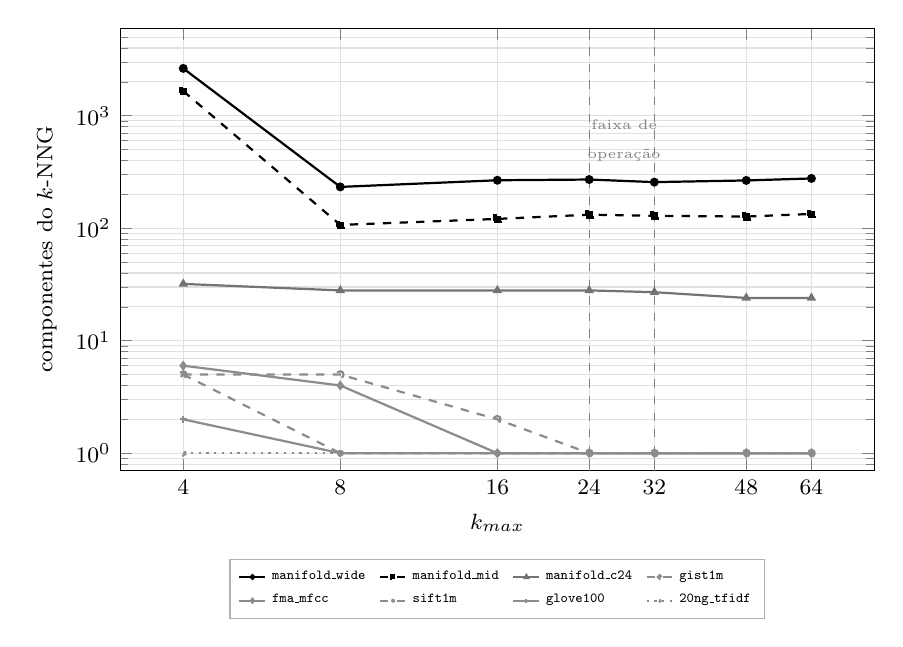
\begin{tikzpicture}
\begin{axis}[
  width=0.92\textwidth, height=7.2cm,
  xlabel={$\kmax$}, ylabel={componentes do $k$-NNG},
  ymode=log, log basis y=10,
  xmode=log, log basis x=2, xtick={4,8,16,24,32,48,64},
  xticklabels={4,8,16,24,32,48,64},
  ymin=0.7, ymax=6000,
  grid=both, grid style={black!12},
  legend style={font=\tiny, at={(0.5,-0.20)}, anchor=north,
                legend columns=4, draw=black!30, legend cell align=left,
                /tikz/every even column/.append style={column sep=1mm}},
  legend image post style={scale=0.55},
  label style={font=\footnotesize}, tick label style={font=\footnotesize},
  every axis plot/.append style={thick, mark size=1.2pt}
]
\addplot[mark=*, black] coordinates {(4,2636)(8,233)(16,267)(24,271)(32,257)(48,266)(64,277)};
\addlegendentry{\texttt{manifold\_wide}}
\addplot[mark=square*, black, dashed] coordinates {(4,1658)(8,107)(16,121)(24,132)(32,129)(48,127)(64,134)};
\addlegendentry{\texttt{manifold\_mid}}
\addplot[mark=triangle*, black!55] coordinates {(4,32)(8,28)(16,28)(24,28)(32,27)(48,24)(64,24)};
\addlegendentry{\texttt{manifold\_c24}}
\addplot[mark=o, black!45, dashed] coordinates {(4,5)(8,5)(16,2)(24,1)(32,1)(48,1)(64,1)};
\addlegendentry{\texttt{gist1m}}
\addplot[mark=diamond*, black!45] coordinates {(4,6)(8,4)(16,1)(24,1)(32,1)(48,1)(64,1)};
\addlegendentry{\texttt{fma\_mfcc}}
\addplot[mark=x, black!45, dashed] coordinates {(4,5)(8,1)(16,1)(24,1)(32,1)(48,1)(64,1)};
\addlegendentry{\texttt{sift1m}}
\addplot[mark=+, black!45] coordinates {(4,2)(8,1)(16,1)(24,1)(32,1)(48,1)(64,1)};
\addlegendentry{\texttt{glove100}}
\addplot[mark=asterisk, black!45, dotted] coordinates {(4,1)(8,1)(16,1)(24,1)(32,1)(48,1)(64,1)};
\addlegendentry{\texttt{20ng\_tfidf}}
\draw[gray, dashed] (axis cs:24,0.7) -- (axis cs:24,6000);
\draw[gray, dashed] (axis cs:32,0.7) -- (axis cs:32,6000);
\node[font=\tiny, gray, anchor=south] at (axis cs:28,620) {faixa de};
\node[font=\tiny, gray, anchor=north] at (axis cs:28,620) {operação};
\end{axis}
\end{tikzpicture}\\
Fonte: Autoral.
\end{figure}

\begin{table}[htb!]
\caption{\label{tab:connectivity} Componentes do \ac{k-NNG} sozinho, em $n$ completo, grafo aproximado, média de 3 sementes. Em negrito, o menor $\kmax$ em que o conjunto se torna conexo.}
\centering
\footnotesize
\begin{tabular}{@{}lrrrrrrr@{}}
\toprule
conjunto de dados & $k=4$ & $k=8$ & $k=16$ & $k=24$ & $k=32$ & $k=48$ & $k=64$ \\
\midrule
\texttt{20ng\_pca500} & \textbf{1} & 1 & 1 & 1 & 1 & 1 & 1 \\
\texttt{20ng\_tfidf}  & \textbf{1} & 1 & 1 & 1 & 1 & 1 & 1 \\
\texttt{glove100}     & 2 & \textbf{1} & 1 & 1 & 1 & 1 & 1 \\
\texttt{sift1m}       & 5 & \textbf{1} & 1 & 1 & 1 & 1 & 1 \\
\texttt{fma\_chroma}  & 8 & 2 & \textbf{1} & 1 & 1 & 1 & 1 \\
\texttt{fma\_mfcc}    & 6 & 4 & \textbf{1} & 1 & 1 & 1 & 1 \\
\texttt{gist1m}       & 5 & 5 & 2 & \textbf{1} & 1 & 1 & 1 \\
\midrule
\texttt{manifold\_mid}  & 1658 & 107 & 121 & 132 & 129 & 127 & 134 \\
\texttt{manifold\_wide} & 2636 & 233 & 267 & 271 & 257 & 266 & 277 \\
\bottomrule
\end{tabular}\\
Fonte: Autoral.
\end{table}

Três observações decorrem desses dados.\\

A primeira observação é que a árvore geradora corrige a fragmentação do grafo de vizinhança e contribui pouco além disso em dados conexos. Onde o \ac{k-NNG} já é um único componente, as pontes não têm o que ligar, do que se poderia concluir que elas não alteram nada. A conectividade sozinha não estabelece isso, e \citeonline{core-sg} já o apontam em termos teóricos: um \ac{k-NNG} conexo pode não conter uma $\mathrm{MST}_{\mpts}$, e os autores exibem um contraexemplo em $k = \mpts = 4$. O que eles estabelecem é a possibilidade; o que esta seção acrescenta é a magnitude. Esse contraexemplo é a configuração em ferradura da Figura \ref{fig:coresg-edge-case}, descrita na Seção \ref{sec:coresg-why}: uma \ac{MST} sobre o grafo completo pode conter uma aresta curta ligando diretamente duas regiões que o \ac{k-NNG} só liga por um desvio longo em torno delas, de modo que os dois grafos são conexos e ainda assim induzem hierarquias diferentes. A Tabela \ref{tab:ablation} resolve a questão diretamente, extraindo uma árvore do \ac{k-NNG} sozinho, sem nenhuma ponte e sem reparo, e pontuando-a contra o \ac{CORE-SG} exato.\\

\begin{table}[htb!]
\caption{\label{tab:ablation} O \ac{k-NNG} sozinho contra o \ac{CORE-SG} exato, com o \ac{k-NNG} mantido exato nos dois lados. A coluna ``divergem'' conta as arestas da árvore exata que este braço não contém, entre as $n-1$ de uma árvore geradora. A razão de peso nunca pode cair abaixo de 1 para uma árvore geradora sobre um subgrafo, de modo que qualquer excesso é um desvio que as arestas do \ac{k-NNG} obrigaram. Duas sementes; $\kmax = 32$ em todas as linhas.}
\centering
\footnotesize
\begin{tabular}{@{}lrrrrrr@{}}
\toprule
 & & \multicolumn{3}{c}{divergem em $\mpts$} & \multicolumn{2}{c}{em $\mpts = \kmax$} \\
\cmidrule(lr){3-5}\cmidrule(lr){6-7}
conjunto de dados & $n$ & $\le 8$ & 16 & 32 & razão de peso & excesso \\
\midrule
\texttt{sift1m}    & 25 mil  & 0 & 1 & 1  & 1,0000027 & 2,7 ppm \\
                   & 50 mil  & 0 & 0 & 4  & 1,0000010 & 1,0 ppm \\
                   & 100 mil & 0 & 0 & 5  & 1,0000008 & 0,8 ppm \\
\texttt{fma\_mfcc} & 25 mil  & 0 & 0 & 8  & 1,0000012 & 1,2 ppm \\
                   & 50 mil  & 0 & 0 & 5  & 1,0000003 & 0,3 ppm \\
                   & 100 mil & 1 & 1 & 9  & 1,0000018 & 1,8 ppm \\
\texttt{glove100}  & 25 mil  & 0 & 2 & 5  & 1,0000043 & 4,3 ppm \\
                   & 50 mil  & 0 & 1 & 6  & 1,0000035 & 3,5 ppm \\
                   & 100 mil & 1 & 4 & 22 & 1,0000052 & 5,2 ppm \\
\midrule
\texttt{gist1m}    & 25 mil  & 0 & 0 & 0  & 1,0000000 & 0 \\
                   & 50 mil  & 0 & 0 & 0  & 1,0000000 & 0 \\
\bottomrule
\end{tabular}\\
Fonte: Autoral.
\end{table}

Da tabela decorrem três constatações, e a primeira é que a forma forte da afirmação é falsa. A razão de peso excede 1 em nove das onze configurações, e como ela não pode cair abaixo de 1 para uma árvore geradora sobre um subgrafo, isso significa que o \ac{k-NNG} sozinho força um desvio em algum lugar. Nas duas configurações restantes, ambas em \texttt{gist1m}, as duas árvores são idênticas aresta a aresta, e a razão é exatamente 1.\\

O efeito é também pequeno e confinado. Em $\mpts \leq 8$ as duas árvores são idênticas em nove das onze configurações, com uma única aresta divergente nas outras duas. Em $\mpts = 16$ elas permanecem idênticas em seis configurações e divergem em 1 a 4 arestas nas cinco restantes. As diferenças se concentram em $\mpts = \kmax$, onde alcançam de 0 a 22 arestas entre 25.000 e 100.000, e de 0,3 a 5,2 partes por milhão do peso total da árvore. Em \texttt{sift1m} com $n = 25.000$, a discrepância inteira é uma única aresta substituída, 18,85 mais pesada que a que ela substituiu, contra uma altura média de fusão de 281,8.\\

A concentração em valores grandes de $\mpts$ é o que a definição prevê. Em $\mpts$ pequeno as \textit{core distances} de \eqref{eq:mrd} são pequenas, de modo que a \textit{mutual reachability distance} é aproximadamente a distância métrica, as arestas mais baratas são as mais curtas, e essas são exatamente as que um \ac{k-NNG} armazena. Em $\mpts = \kmax$ as \textit{core distances} estão em seu maior valor, e todo ponto a distância menor que $\coredist^{\kmax}(x)$ de $x$ é um parceiro igualmente barato, ao mesmo peso; mas a fronteira dessa bola é justamente o $\kmax$-ésimo vizinho armazenado, de modo que parceiros empatados naquela distância são igualmente baratos e não couberam na lista. O conjunto \texttt{glove100} exibe o efeito com maior intensidade e é também o de maior dimensionalidade intrínseca entre os avaliados, onde tais empates são mais numerosos. Essa é a leitura que o padrão sustenta, e permanece uma conjectura: as arestas divergentes não foram inspecionadas individualmente.\\

A consequência prática é a mesma que motivou o projeto. As pontes rendem em uma faixa estreita próxima a $\mpts = \kmax$, e os agrupamentos planos cortados das duas árvores foram idênticos em todos os limiares aplicados. Derivar a rotulação de componentes custa de 0,08 a 3,5\,ms nos conjuntos avaliados, contra 5,3 a 222\,ms de trabalho de \textit{hubness} e de pontes, um fator de 48 a 136, de modo que testar a conectividade primeiro e pular o cálculo das pontes onde o grafo já é conexo custa pouco e abre mão de pouco.\\

Onde o grafo de fato se fragmenta, o quadro é inteiramente diferente, e é esse o controle de que a ablação precisa. Em \texttt{manifold\_mid} o \ac{k-NNG} sozinho deixa 150 componentes em todos os tamanhos testados, de modo que a estrutura extraída dele é uma floresta com 149 arestas a menos do que uma árvore geradora exigiria, e sua razão de peso, de 0,92 a 0,97, fica abaixo de 1 apenas porque é uma soma sobre menos arestas. Ali as pontes deixam de ser uma correção marginal e passam a ser o mecanismo que produz a árvore.\\

A segunda é que a dimensionalidade ambiente não prediz o limiar, como mostra o par de conjuntos destacado na legenda da Figura \ref{fig:components}. O que distingue os dois casos é a presença de componentes genuinamente separados por densidade, cada um contendo muitos pontos, propriedade que a família sintética possui por construção e que os dados reais, nessas escalas, majoritariamente não possuem.\\

A terceira é que a conectividade observada não vem da aproximação. Ela poderia ser um erro residual do NN-Descent, na forma de arestas longas entre componentes que conectassem um grafo que o \ac{k-NNG} exato deixaria em pedaços, e a medição afasta essa leitura. Na faixa de operação, o conjunto \texttt{manifold\_c24} produz 24 componentes com o grafo exato e de 25 a 29 com o aproximado, já que um vizinho não encontrado remove uma aresta enquanto um vizinho substituído permanece local. O efeito se inverte quando $\kmax$ se aproxima do tamanho do componente, caso de \texttt{manifold\_c32} em $\kmax = 64$, com 30 componentes no grafo aproximado contra 32 no exato, e por isso a afirmação é enunciada de forma restrita.\\

% =====================================================================
% =====================================================================
\section{Memória por dispositivo contra quantidade de instâncias\label{sec:res-memory}}
% =====================================================================

Esta seção responde à QP1. A Tabela \ref{tab:memory} reporta uma construção de $5 \times 10^5$ pontos em contagens de instâncias de 1 a 64, medida em quatro \ac{GPU}s com a sobreposição padrão $\omega = 1{,}0$. A grandeza reportada é a maior instância que um dispositivo precisou manter, que é o que decide se uma configuração cabe.\\

\begin{table}[htb!]
\caption{\label{tab:memory} Uma construção de \texttt{sift1m} e \texttt{glove100} em $n = 5 \times 10^5$, $\kmax = 32$, $\omega = 1{,}0$, em quatro \ac{GPU}s. A coluna \textit{residente} é a maior instância que um dispositivo precisou manter, e \textit{fator} é sua redução contra $m = 1$. A revocação é amostrada sobre 2.000 consultas pontuadas exatamente contra todos os pontos. Em negrito, o extremo de cada coluna: a maior revocação de cada conjunto, o maior fator de redução e a menor residência.}
\centering
\footnotesize
\begin{tabular}{@{}lrrrrr@{}}
\toprule
 & & \multicolumn{2}{c}{\texttt{sift1m}} & \multicolumn{2}{c}{\texttt{glove100}} \\
\cmidrule(lr){3-4}\cmidrule(lr){5-6}
instâncias & fator & residente & revocação & residente & revocação \\
\midrule
1  & 1,0$\times$  & 472,0\,MB & 0,9677 & 424,0\,MB & 0,7188 \\
2  & 1,4$\times$  & 329,1\,MB & \textbf{0,9814} & 295,6\,MB & 0,7799 \\
4  & 2,4$\times$  & 196,5\,MB & 0,9785 & 176,5\,MB & \textbf{0,7890} \\
8  & 4,4$\times$  & 107,7\,MB & 0,9741 & 96,7\,MB  & 0,7773 \\
16 & 8,4$\times$  & 56,4\,MB  & 0,9702 & 50,7\,MB  & 0,7646 \\
32 & 16,3$\times$ & 28,9\,MB  & 0,9669 & 25,9\,MB  & 0,7476 \\
64 & \textbf{32,3}$\times$ & \textbf{14,6\,MB} & 0,9645 & \textbf{13,1\,MB} & 0,7289 \\
\bottomrule
\end{tabular}\\
Fonte: Autoral.
\end{table}

A residência segue a Equação \eqref{eq:instancesize}: 472,0\,MB em uma instância e 14,6\,MB em 64, um fator de 32,3. O fator é 32 e não 64 porque $\omega = 1{,}0$ dobra o tamanho de cada instância, deixando $m = 1$ inalterado, caso em que os sorteios de sobreposição recaem sobre o próprio bloco único. Em $\omega = 0{,}05$ a mesma faixa produz 472,0\,MB contra 7,7\,MB, um fator de 61,0. As razões se mantêm em \texttt{glove100} e em toda contagem de dispositivos medida, já que a residência é determinada pela quantidade de instâncias e não por quantos dispositivos as executam.\\

A revocação não cai monotonicamente. Ela sobe de $m = 1$ para $m = 2$ nos dois conjuntos, em 0,0137 em \texttt{sift1m} e 0,0611 em \texttt{glove100}, atinge máximo em $m = 2$ no primeiro e em $m = 4$ no segundo, e declina a partir daí. Em $m = 1$ nenhum passo de reparo é executado. Em \texttt{glove100} toda contagem de 2 a 64 permanece acima do valor de $m = 1$, em 0,0702 no máximo e 0,0101 em $m = 64$; em \texttt{sift1m} as contagens de 2 a 16 permanecem acima, e $m = 32$ e $m = 64$ ficam 0,0008 e 0,0032 abaixo.\\

Esse comportamento contraria a expectativa. Particionar um conjunto de dados para construir um grafo de vizinhança deveria, pelo argumento da Seção \ref{sec:problem-partition-cost}, apenas piorar o resultado. O que a tabela mostra é que o passo de reparo, operando sobre um grafo mesclado que já possui vizinhanças razoáveis, encontra arestas que uma descida única partindo de um grafo aleatório não encontra dentro do mesmo orçamento de rodadas. A decomposição, portanto, não troca apenas qualidade por memória: em contagens baixas de instâncias ela melhora as duas.\\

O custo em tempo de relógio da mesma faixa é de 5,862\,s em $m = 1$ contra 10,033\,s em $m = 64$ em \texttt{sift1m}, um fator de 1,71. Em uma única \ac{GPU} a mesma comparação é de 5,757\,s contra 15,774\,s, um fator de 2,74; a Seção \ref{sec:res-overlap} separa as duas.\\

% =====================================================================
\section{Sobreposição de instâncias\label{sec:res-overlap}}
% =====================================================================

Esta seção responde à QP2. A fração de sobreposição $\omega$ da Equação \eqref{eq:instancesize} determina quantos pontos uma instância carrega além do seu próprio bloco. A Tabela \ref{tab:overlap} compara pares de configurações que colocam quantidades comparáveis de memória em um dispositivo, obtidos dobrando $m$ junto com $\omega$.\\

\begin{table}[htb!]
\caption{\label{tab:overlap} Configurações de residência comparável, quatro \ac{GPU}s, $n = 5 \times 10^5$, $\kmax = 32$. Cada par dobra a quantidade de instâncias junto com a sobreposição. Em negrito, a configuração vencedora de cada par em revocação e em tempo total.}
\centering
\footnotesize
\begin{tabular}{@{}llrrr@{}}
\toprule
conjunto & configuração & residente & revocação & total \\
\midrule
\texttt{sift1m}
  & $m = 8$, $\omega = 0{,}05$  & 61,6\,MB  & 0,9672 & 10,36\,s \\
  & $m = 16$, $\omega = 1{,}00$ & 56,4\,MB  & \textbf{0,9702} & \textbf{10,02\,s} \\
\addlinespace[1pt]
  & $m = 16$, $\omega = 0{,}05$ & 30,9\,MB  & 0,9594 & 10,54\,s \\
  & $m = 32$, $\omega = 1{,}00$ & 28,9\,MB  & \textbf{0,9669} & \textbf{9,20\,s} \\
\addlinespace[1pt]
  & $m = 32$, $\omega = 0{,}05$ & 15,5\,MB  & 0,9493 & 10,20\,s \\
  & $m = 64$, $\omega = 1{,}00$ & 14,6\,MB  & \textbf{0,9645} & \textbf{10,03\,s} \\
\midrule
\texttt{glove100}
  & $m = 4$, $\omega = 0{,}05$  & 110,0\,MB & 0,7492 & 8,44\,s \\
  & $m = 8$, $\omega = 1{,}00$  & 96,7\,MB  & \textbf{0,7773} & \textbf{7,84\,s} \\
\addlinespace[1pt]
  & $m = 8$, $\omega = 0{,}05$  & 55,3\,MB  & 0,7317 & \textbf{8,19\,s} \\
  & $m = 16$, $\omega = 1{,}00$ & 50,7\,MB  & \textbf{0,7646} & 9,32\,s \\
\addlinespace[1pt]
  & $m = 16$, $\omega = 0{,}05$ & 27,8\,MB  & 0,7037 & 9,60\,s \\
  & $m = 32$, $\omega = 1{,}00$ & 25,9\,MB  & \textbf{0,7476} & \textbf{9,05\,s} \\
\addlinespace[1pt]
  & $m = 32$, $\omega = 0{,}05$ & 13,9\,MB  & 0,6745 & \textbf{9,50\,s} \\
  & $m = 64$, $\omega = 1{,}00$ & 13,1\,MB  & \textbf{0,7289} & 9,67\,s \\
\bottomrule
\end{tabular}\\
Fonte: Autoral.
\end{table}

O braço de $\omega = 1{,}00$ ocupa menos memória no dispositivo e alcança revocação maior nos sete pares: de 0,0029 a 0,0152 em \texttt{sift1m} e de 0,0281 a 0,0544 em \texttt{glove100}. O tempo total cai em cinco dos sete e sobe em dois.\\

O comportamento em tempo decorre de onde cada fase executa. Ao longo dos sete pares, o passo de reparo é de 2,5\% a 30,0\% mais curto em $\omega = 1{,}00$ e a fase de instâncias de 72\% a 87\% mais longa, de modo que a troca só compensa quando há dispositivos para dividir a fase maior. Em $m = 64$ em \texttt{sift1m}, uma \ac{GPU} leva 13,41\,s em $\omega = 0{,}05$ e 15,77\,s em $\omega = 1{,}00$; quatro \ac{GPU}s levam 10,26\,s e 10,03\,s.\\

Elevar $\omega$ também eleva a parcela da construção que os dispositivos executam. Em $m \ge 8$, a fase de instâncias acelera de 3,83 a 3,87 vezes em quatro dispositivos sob $\omega = 0{,}05$, e de 3,94 a 3,99 sob $\omega = 1{,}00$ em \texttt{sift1m}; em \texttt{glove100}, de 3,82 a 3,91 contra 3,90 a 3,98. Em $m = 64$ sobre quatro dispositivos, a fração paralela $f$ sobe de 0,100 para 0,189 em \texttt{sift1m} e de 0,104 para 0,208 em \texttt{glove100}.\\

Uma configuração intermediária foi medida em \texttt{sift1m}. Em $\omega = 0{,}50$ a fronteira situa-se entre as duas, e a construção particionada mais rápida de toda a grade está ali: 8,13\,s com revocação 0,9694 e 84,1\,MB residentes, em $m = 8$. A configuração mais rápida e a mais precisa a uma dada residência não coincidem.\\

% =====================================================================
\section{Construção em escala\label{sec:res-scale}}
% =====================================================================

A Tabela \ref{tab:scale} reporta construções únicas de $10^7$ a $5 \times 10^7$ pontos em $d = 32$, com a quantidade de instâncias elevada em proporção a $n$.\\

\begin{table}[htb!]
\caption{\label{tab:scale} Construções únicas sobre dados sintéticos, $d = 32$, $\kmax = 32$, quatro \ac{GPU}s, $m = n / 5 \times 10^5$, $\omega = 0{,}05$. Nenhum dispositivo esgotou a memória em qualquer configuração.}
\centering
\footnotesize
\begin{tabular}{@{}lrrrrr@{}}
\toprule
$n$ & $m$ & total & residente & hospedeiro & revocação \\
\midrule
$1\times10^7$ & 20  & 209,5\,s  & 293,3\,MB & 10,5\,GB & 0,9993 \\
$2\times10^7$ & 40  & 392,4\,s  & 293,7\,MB & 20,5\,GB & 0,9987 \\
$3\times10^7$ & 60  & 581,8\,s  & 293,8\,MB & 30,6\,GB & 0,9987 \\
$4\times10^7$ & 80  & 838,9\,s  & 293,8\,MB & 40,7\,GB & 0,9985 \\
$5\times10^7$ & 100 & 1090,2\,s & 293,9\,MB & 50,5\,GB & 0,9970 \\
\bottomrule
\end{tabular}\\
Fonte: Autoral.
\end{table}

A residência por dispositivo varia em 0,6\,MB ao longo de um aumento de cinco vezes em $n$, ao passo que a memória do hospedeiro cresce linearmente, a 1001 bytes por ponto. A revocação cai de 0,9993 para 0,9970 na mesma faixa. A construção de $5 \times 10^7$ pontos conclui em 18,2 minutos.\\

Uma construção de instância única sobre os mesmos dados exige 560 bytes por ponto no dispositivo, o que coloca $5 \times 10^7$ pontos em 28,0\,GB e $10^7$ em 5,6\,GB. A construção de instância única em $10^7$ pontos foi executada para confirmar a aritmética: ela colocou 5,600\,GB em um acelerador, não reportou nenhuma instância sem memória e concluiu em 119,2\,s. Os tamanhos maiores excedem o dispositivo de 8\,GB.\\

Um grafo sobre $5 \times 10^7$ pontos não é construído mais rápido pela decomposição: ele passa a ser construível, no mesmo hardware em que antes não era. A Seção \ref{sec:disc-category} retoma a distinção.\\

% =====================================================================
\section{Escalabilidade em múltiplos aceleradores\label{sec:res-scaling}}
% =====================================================================

A Tabela \ref{tab:scaling} reporta a fase de instâncias e a construção inteira contra a quantidade de dispositivos, em contagens de instâncias fixas.\\

\begin{table}[htb!]
\caption{\label{tab:scaling} \texttt{sift1m} em $n = 5 \times 10^5$, $\kmax = 32$, $\omega = 0{,}05$. A coluna \textit{instâncias} é a fase executada nos dispositivos; \textit{total} inclui as fases do hospedeiro. A Seção \ref{sec:res-overlap} reporta a mesma medição em $\omega = 1{,}00$.}
\centering
\footnotesize
\begin{tabular}{@{}lrrrrr@{}}
\toprule
 & \multicolumn{2}{c}{$m = 16$} & \multicolumn{2}{c}{$m = 64$} & \\
\cmidrule(lr){2-3}\cmidrule(lr){4-5}
\ac{GPU}s & instâncias & total & instâncias & total & $f$ \\
\midrule
1 & 4,053\,s & 12,780\,s & 3,897\,s & 13,435\,s & 0,290 \\
2 & 2,040\,s & 12,031\,s & 1,943\,s & 11,919\,s & 0,163 \\
3 & 1,523\,s & 10,049\,s & 1,329\,s & 11,888\,s & 0,112 \\
4 & 1,041\,s & 9,549\,s & 1,025\,s & 10,521\,s & 0,097 \\
\bottomrule
\end{tabular}\\
Fonte: Autoral.
\end{table}

A fase de instâncias cai de 3,897\,s para 1,025\,s em $m = 64$, uma aceleração de 3,80 em quatro dispositivos. A construção inteira cai de 13,435\,s para 10,521\,s, uma aceleração de 1,28.\\

A diferença entre os dois números decorre da parcela da construção que os dispositivos executam. Em $m = 64$ sobre uma \ac{GPU}, a fase de instâncias é 0,290 do total; sobre quatro, é 0,097, porque essa fase encolhe enquanto as fases do hospedeiro não. Em $n = 5 \times 10^7$ a fase de instâncias é de 123,4\,s em 1090,2\,s, ou 0,113, e o passo de reparo é de 863,0\,s, ou 0,792.\\

Pela lei de Amdahl \cite{amdahl}, uma fração paralela de 0,097 limita a aceleração alcançável a 1,11 por mais dispositivos que se acrescente. A eficiência da fase paralela alcança 3,80 de 4,00 possíveis, de modo que o limite à escalabilidade está no tamanho relativo da fase sequencial. Essa fase é o passo de reparo, e a seção seguinte o examina.\\

% =====================================================================
\section{O passo de reparo\label{sec:res-repair}}
% =====================================================================

O passo de reparo é a maior fase isolada de uma construção e executa no hospedeiro. A Tabela \ref{tab:refine} reporta a revocação contra a quantidade de rodadas de NN-Descent que lhe é permitida.\\

\begin{table}[htb!]
\caption{\label{tab:refine} \texttt{sift1m} em $n = 5 \times 10^5$, $m = 8$, $\omega = 0{,}05$, quatro \ac{GPU}s. As rodadas são o teto de iterações do passo de reparo; cinco é o padrão.}
\centering
\footnotesize
\begin{tabular}{@{}lrrrr@{}}
\toprule
rodadas & reparo & total & $f$ & revocação \\
\midrule
1 & 0,835\,s & 2,963\,s & 0,376 & 0,2219 \\
2 & 3,502\,s & 5,625\,s & 0,199 & 0,6556 \\
3 & 5,206\,s & 7,345\,s & 0,154 & 0,8942 \\
5 & 7,304\,s & 9,423\,s & 0,118 & 0,9671 \\
\bottomrule
\end{tabular}\\
Fonte: Autoral.
\end{table}

Reduzir o passo de cinco rodadas para uma diminui o tempo de construção em 68,6\% e a revocação em 0,7452. A relação é fortemente não linear: a maior parte da revocação final é produzida pelas duas últimas rodadas, porque as primeiras estabelecem as vizinhanças das quais as seguintes dependem.\\

As outras três estratégias da Seção \ref{sec:discarded-repair} foram medidas da seguinte forma.\\

Restringir o passo aos vértices que a mesclagem alterou deixa o conjunto ativo em $5 \times 10^5$ de $5 \times 10^5$ vértices. A razão é estrutural: uma construção parte de um grafo vazio, de modo que toda aresta aceita na mesclagem é uma inserção, e o conjunto de vértices alterados é o conjunto inteiro.\\

Executar o passo como instâncias sobre blocos crescidos por localidade estagia 478.591 vértices em quatro blocos e 1.265.903 em 32, para um conjunto de $2 \times 10^5$ pontos, isto é, de 2,4 a 6,3 vezes $n$. A maior instância assim produzida ocupa 150,0\,MB contra 49,0\,MB das instâncias de descida da mesma construção, de modo que a estratégia piora a grandeza que o método existe para controlar. Omitir os fechos dos blocos torna a decomposição viável em memória, mas derruba a revocação para 0,8748 em quatro blocos e 0,6088 em dezesseis.\\

A fusão simétrica de \citeonline{knn_merge}, executada no lugar do passo, foi medida em \texttt{sift1m} com $n = 5 \times 10^5$ e oito instâncias em um dispositivo, contra um passo de 3,85\,s a 0,9672 de revocação. Ela alcança 2,82\,s a 0,9412, 2,22\,s a 0,8735 e 1,52\,s a 0,6099 conforme o prefixo retido cai de três quartos da lista para um quarto. Truncar apenas a varredura de candidatos, sem o preenchimento nem o filtro entre blocos, alcança 3,02\,s a 0,9416, 2,15\,s a 0,8729 e 0,97\,s a 0,6043 nos mesmos três comprimentos de prefixo: em oito instâncias, os dois mecanismos adicionais não respondem por nada do efeito. Em duas instâncias, que é o caso de dois conjuntos para o qual o algoritmo é derivado, o filtro entre blocos vale 14\% do passo por 0,004 de revocação. Nenhum comprimento de prefixo alcança a revocação da varredura completa.\\

Nenhuma das quatro estratégias encurta o passo a revocação constante. O que o reduz é a sobreposição da Seção \ref{sec:res-overlap}, que desloca parte de seu trabalho para as instâncias, isto é, para os dispositivos, mantendo o tamanho do passo.\\

% =====================================================================
\section{Comparação com uma construção em GPU: cuML\label{sec:res-cuml}}
% =====================================================================

A biblioteca cuML \cite{cuml} implementa o \ac{HDBSCAN*} em \ac{GPU}. A Tabela \ref{tab:cuml} compara uma construção contra um ajuste da cuML no mesmo dispositivo e sobre os mesmos dados.\\

\begin{table}[htb!]
\caption{\label{tab:cuml} \texttt{sift1m}, um dispositivo, $\kmax = 32$ para este trabalho e $\mpts = 10$ para a cuML.}
\centering
\footnotesize
\begin{tabular}{@{}lrrr@{}}
\toprule
$n$ & este trabalho & cuML & aceleração \\
\midrule
$5\times10^5$ & 9,63\,s  & 43,57\,s  & 4,53$\times$ \\
$1\times10^6$ & 17,99\,s & 180,03\,s & 10,01$\times$ \\
\bottomrule
\end{tabular}\\
Fonte: Autoral.
\end{table}

Ao dobrar $n$, o custo deste trabalho cresce por um fator de 1,87 e o da cuML por 4,13. Em um conjunto de dimensionalidade 32, a cuML esgota um dispositivo de 8\,GB em $8 \times 10^6$ pontos, ponto em que a residência por dispositivo deste trabalho, em $5 \times 10^7$ pontos da mesma dimensionalidade, é de 293,9\,MB.\\

As duas comparações são de naturezas distintas. A primeira mede quanto mais rápido o método é; a segunda determina se o conjunto pode ser processado.\\

% =====================================================================
\section{O custo de uma consulta\label{sec:res-extract}}
% =====================================================================

Um \ac{CORE-SG} construído responde a uma consulta pela $\mathrm{MST}_{\mpts}$ repesando suas arestas armazenadas com $\mrd^{\mpts}$ e executando um algoritmo de árvore geradora sobre elas. A Tabela \ref{tab:extract} reporta esse custo e o da varredura inteira sobre $\mpts \in [1, \kmax]$, contra $n$.\\

\begin{table}[htb!]
\caption{\label{tab:extract} Custo de extração em um dispositivo, $\kmax = 32$. A coluna \textit{arestas} é a quantidade de arestas não direcionadas armazenadas. A coluna \textit{uma consulta} é a média sobre $\mpts \in [2, 32]$; a primeira extração após uma construção é excluída dela, por pagar o primeiro acesso aos arranjos. A coluna \textit{32 valores} é o total medido, incluindo essa primeira extração. As linhas são médias de 3 sementes, exceto $10^7$, que é uma.}
\centering
\footnotesize
\begin{tabular}{@{}lrrr@{}}
\toprule
$n$ & arestas & uma consulta & 32 valores \\
\midrule
$2\times10^5$ & 5,21\,M   & 0,216\,s & 6,92\,s   \\
$5\times10^5$ & 13,10\,M  & 0,437\,s & 14,15\,s  \\
$1\times10^6$ & 26,50\,M  & 0,853\,s & 27,60\,s  \\
$1\times10^7$ & 224,57\,M & 9,57\,s  & 310,83\,s \\
\bottomrule
\end{tabular}\\
Fonte: Autoral.
\end{table}

O custo por aresta armazenada permanece entre $3{,}2$ e $5{,}0 \times 10^{-8}$\,s ao longo de uma faixa de 438 vezes na quantidade de arestas, de modo que a extração é linear nas $O(n\kmax)$ arestas que ela percorre, antes que em $n$ isoladamente. O conjunto \texttt{glove100} em $n = 5 \times 10^5$ concorda com \texttt{sift1m} no mesmo $n$: 13,58\,M arestas contra 13,10\,M, e 0,471\,s contra 0,437\,s.\\

Dentro de um mesmo grafo, o custo cai conforme $\mpts$ sobe. Em $n = 10^6$ ele é de 1,060\,s em $\mpts = 2$ e de 0,791\,s em $\mpts = 32$, uma queda de 25\%. A consulta mais cara é, portanto, a de menor $\mpts$.\\

A varredura inteira custa de 1,08 a 1,72 vezes a construção que produziu o grafo, na mesma execução e no mesmo dispositivo. Contra a construção de uma árvore sobre o grafo completo para cada valor, medida no único tamanho em que essa referência é acessível, a varredura é de 161 a 167 vezes mais barata: 0,82\,s contra 134\,s em $n = 2 \times 10^4$, onde a referência é extrapolada a partir de 3 das 32 árvores exatas.\\

Posto ao lado da Tabela \ref{tab:cuml}, um ajuste da cuML em $n = 10^6$ custa 180,03\,s e uma extração de um \ac{CORE-SG} já construído, nesse mesmo tamanho, custa 0,853\,s. Uma varredura de 32 valores são 32 ajustes para a cuML e uma construção somada a 27,60\,s aqui.\\

Essa seção fornece também uma verificação das pontes em escalas que a referência exata não alcança. Em todas as 480 extrações realizadas (todo $\mpts$, em todo conjunto de dados, até $10^7$ pontos), a árvore extraída possui exatamente $n - 1$ arestas e um único componente. A estimativa de pontes, somada ao reparo de conectividade, produziu uma árvore geradora em todos os casos medidos, sem nenhuma floresta.\\

% =====================================================================
\section{O ganho da varredura de $\mpts$ sobrevive à decomposição\label{sec:res-mpts}}
% =====================================================================

O \ac{CORE-SG} existe para servir toda a faixa $\mpts \in [1, \kmax]$ a partir de um único grafo. A Tabela \ref{tab:mpts} verifica que essa propriedade é preservada quando o grafo é construído incrementalmente em vez de de uma só vez.\\

\begin{table}[htb!]
\caption{\label{tab:mpts} Extração de todas as \ac{MST}s para $\mpts \in [1, \kmax]$ a partir de um único \ac{CORE-SG}, contra o cálculo de cada uma a partir do grafo completo.}
\centering
\footnotesize
\begin{tabular}{@{}lrrr@{}}
\toprule
conjunto de dados & varredura no CORE-SG & varredura no grafo completo & aceleração \\
\midrule
\texttt{20ng\_pca500}   & 0,286\,s & 86,9\,s  & 303$\times$ \\
\texttt{fma\_mfcc}      & 0,831\,s & 153,7\,s & 185$\times$ \\
\texttt{sift1m}         & 0,814\,s & 138,3\,s & 170$\times$ \\
\texttt{manifold\_exact}& 0,074\,s & 5,2\,s   & 71$\times$ \\
\bottomrule
\end{tabular}\\
Fonte: Autoral.
\end{table}

Os valores são consistentes com a faixa reportada pelo trabalho original \cite{core-sg}, e o ponto desta dissertação é que eles são preservados depois de o grafo ser construído por instâncias independentes. Nenhuma das linhas de base externas possui equivalente para essa propriedade: o cuML exige um ajuste completo por valor de $\mpts$, e o FISHDBC serve um único valor.\\

% =====================================================================
\section{Concordância entre os ambientes de execução\label{sec:res-parity}}
% =====================================================================

A Tabela \ref{tab:parity} compara construções nos ambientes de \ac{CPU} e \ac{CUDA} a partir dos mesmos dados e da mesma semente.\\

\begin{table}[htb!]
\caption{\label{tab:parity} $n = 5 \times 10^4$, 3 sementes. A razão de peso compara a $\mathrm{MST}_{8}$ extraída dos dois grafos.}
\centering
\footnotesize
\begin{tabular}{@{}lrrr@{}}
\toprule
conjunto & revocação \ac{CPU} & revocação \ac{CUDA} & razão de peso \\
\midrule
\texttt{sift1m}        & 0,9911 & 0,9911 & 0,999998 \\
\texttt{manifold\_mid} & 0,9948 & 0,9944 & 0,996796 \\
\bottomrule
\end{tabular}\\
Fonte: Autoral.
\end{table}

A revocação difere em no máximo 0,0004 e as árvores extraídas diferem em no máximo 0,32\% no peso total. As afirmações do trabalho não dependem, portanto, do ambiente de execução, o que importa porque a decomposição em instâncias é uma propriedade do algoritmo, não do hardware que a executa.\\

% =====================================================================
\section{Sensibilidade a parâmetros\label{sec:res-sensitivity}}
% =====================================================================

\subsection{Cota por componente\label{sec:res-quota}}

Os parâmetros de cobertura de anti-hubs não produzem sinal em dados cujo \ac{k-NNG} é conexo, o que, conforme a Seção \ref{sec:res-connectivity}, é todo conjunto de dados real. Reexecutados sobre dados que se fragmentam, o resultado é positivo.\\

A cota por componente, definida na Seção \ref{sec:quota}, é a quantidade mínima de anti-hubs que cada componente do \ac{k-NNG} contribui independentemente da seleção global, e existe para impedir que componentes pequenos sejam ignorados. Ela é determinante nos dados que se fragmentam. Em $n = 50.000$, o \ac{k-NNG} de \texttt{manifold\_wide} se divide em 300 componentes, e as pontes o reduzem a um em toda cota a partir de 1, inclusive quando a contagem de anti-hubs é reduzida à metade. Com a cota desativada por completo, as pontes deixam em média 12 componentes sem ligação, com 9, 10 e 17 nas três sementes, porque um componente que não recebe nenhum anti-hub não tem de onde partir uma ponte. O conjunto \texttt{manifold\_mid} se comporta da mesma maneira em magnitude menor, com média de 2,3 componentes remanescentes sem a cota, entre 1 e 4 conforme a semente, contra exatamente 1 com ela. A contagem de 300 componentes difere das 271 reportadas na Tabela \ref{tab:connectivity} porque aquela medição usa $n = 100.000$: com menos pontos por grupo, o grafo de vizinhança se fragmenta mais. O orçamento global é, portanto, suficiente para a cobertura apenas em combinação com a cota, e um anti-hub por componente basta.\\

\subsection{Dimensionalidade ambiente contra dimensionalidade intrínseca\label{sec:res-dimension}}

O termo de dimensionalidade na contagem de anti-hubs pesa mais. A dimensionalidade ambiente $d$ é o número de coordenadas que cada ponto carrega, em contraste com a dimensionalidade intrínseca da variedade que os dados ocupam. A Tabela \ref{tab:budget-fraction} apresenta a fração de $n$ selecionada como anti-hubs sob cada regra.\\

\begin{table}[htb!]
\caption{\label{tab:budget-fraction} Fração de $n$ selecionada como anti-hubs sob cada regra de dimensionamento. A coluna ``ambiente+lim.'' aplica o limitador de custo em operações de par sobre a regra ambiente. Em negrito, os casos em que a regra seleciona todos os pontos e a estimativa degenera na \ac{MST} exata.}
\centering
\footnotesize
\begin{tabular}{@{}lrrrr@{}}
\toprule
conjunto de dados & ambiente & ambiente+lim. & intrínseca & intrínseca $\times 4$ \\
\midrule
\texttt{20ng\_tfidf} ($d=1000$)  & \textbf{1,000} & 0,500 & 0,118 & 0,472 \\
\texttt{20ng\_pca500} ($d=500$)  & \textbf{1,000} & 0,707 & 0,102 & 0,408 \\
\texttt{gist1m} ($d=960$)        & \textbf{1,000} & 0,510 & 0,070 & 0,280 \\
\texttt{sift1m} ($d=128$)        & 0,368 & 0,368 & 0,029 & 0,115 \\
\texttt{manifold\_c24} ($d=64$)  & 0,177 & 0,177 & 0,014 & 0,044 \\
\bottomrule
\end{tabular}\\
Fonte: Autoral.
\end{table}

Nos experimentos realizados, usar o $d$ ambiente em $\lceil d \ln|E| \rceil$ selecionou 100\% dos pontos nos três conjuntos de dados com $d \geq 500$, de modo que a estimativa degenerou na \ac{MST} exata, e de 17,7 a 36,8\% nos demais conjuntos avaliados, dos quais a Tabela \ref{tab:budget-fraction} apresenta dois. Nenhuma dessas frações é sublinear em qualquer sentido útil. Substituí-lo por uma dimensionalidade intrínseca estimada gratuitamente a partir dos raios de vizinhança já armazenados \cite{levina_bickel}, agregada pela média harmônica \cite{mackay_ghahramani}, usa de 1,4 a 11,8\% e executa de 3,2 a 35,9 vezes mais rápido. As dimensionalidades intrínsecas medidas expõem a magnitude da discrepância: 10,2 para SIFT contra $d = 128$ ambiente, 28,5 para GIST contra 960, 34,5 para GloVe contra 100, e 36,3 para 20NG em representação TF-IDF contra 1000.\\

A troca não é gratuita, e a Tabela \ref{tab:budget-quality} apresenta o outro lado dela, restrita aos conjuntos em que as pontes são determinantes.\\

\begin{table}[htb!]
\caption{\label{tab:budget-quality} Pior razão de peso da árvore geradora sob cada regra de dimensionamento, restrita aos conjuntos de dados cujo \ac{k-NNG} se fragmenta. Em negrito, a regra mais precisa em cada linha.}
\centering
\footnotesize
\begin{tabular}{@{}lrrrr@{}}
\toprule
conjunto de dados & ambiente & intrínseca & intrínseca $\times 2$ & intrínseca $\times 4$ \\
\midrule
\texttt{manifold\_c24}   & \textbf{1,00021} & 1,01461 & 1,00858 & 1,00356 \\
\texttt{manifold\_c32}   & \textbf{1,00020} & 1,01149 & 1,00694 & 1,00476 \\
\texttt{manifold\_exact} & \textbf{1,00000} & 1,00736 & 1,00332 & 1,00133 \\
\texttt{manifold\_c8}    & \textbf{1,00001} & 1,00192 & 1,00074 & 1,00033 \\
\bottomrule
\end{tabular}\\
Fonte: Autoral.
\end{table}

A dimensionalidade ambiente é a regra mais precisa. Ela é também de 3 a 36 vezes mais cara e degenerada em alta dimensionalidade. O multiplicador recupera a maior parte da diferença: com fator 4, a razão de peso fica entre 0,03\% e 0,48\% do exato enquanto ainda usa uma fração do orçamento. A leitura correta é uma troca entre custo e precisão. O limitador de custo sozinho é insuficiente, pois ainda seleciona 51\% de $n$ em \texttt{gist1m}, mas vale ser mantido para os casos em que o estimador de dimensionalidade não for confiável.\\



% ----------------------------------------------------------
% Discussão e Trabalhos Futuros
% ----------------------------------------------------------
% ---
% Capitulo de Discussao
% ---

\chapter{Discussão e Trabalhos Futuros\label{cha:discussion}}

% =====================================================================
\section{Síntese dos resultados\label{sec:disc-summary}}
% =====================================================================

As quatro questões de pesquisa da Seção \ref{sec:research-questions} podem agora ser respondidas.\\

\textbf{QP1, sobre a decomposição.} A construção do \ac{CORE-SG} admite decomposição em subproblemas cuja memória individual é controlável de forma independente de $n$. A maior instância residente cai de 472,0\,MB para 14,6\,MB conforme a contagem de instâncias sobe de 1 para 64, e permanece em 293\,MB enquanto o conjunto de dados cresce de $10^7$ para $5 \times 10^7$ pontos, bastando para isso elevar a contagem de instâncias em proporção a $n$. A Equação \eqref{eq:devicecost} torna o par $(m, \omega)$ que cabe em um dado acelerador calculável em vez de descoberto por tentativa. As instâncias não se comunicam durante a execução, de modo que o escalonamento entre dispositivos não exige protocolo algum.\\

\textbf{QP2, sobre o custo em qualidade.} O particionamento deixa pares não comparados, e esse déficit é real, mas é recuperável e controlável. Um passo de reparo sobre o grafo mesclado o recupera; a fração de sobreposição o reduz antes que ele ocorra. A decomposição não é uma concessão pura: em contagens baixas de instâncias a revocação \textit{sobe} em relação a uma construção não particionada, porque o reparo, operando sobre um grafo que já possui vizinhanças razoáveis, encontra arestas que uma descida única partindo do acaso não encontra no mesmo orçamento. Em residência equiparada, elevar a sobreposição domina a alternativa nos sete pares medidos.\\

\textbf{QP3, sobre a árvore geradora.} A metade de árvore geradora pode ser substituída por uma estimativa cujo conjunto abrangido é dimensionado pela dimensionalidade e pela quantidade de arestas, independentemente de $n$. As árvores estimadas são no máximo 0,024\% mais pesadas que as exatas, produzem agrupamentos planos idênticos, e custam de 10,5 a 36 vezes menos. Em escala, a etapa de pontes é de 0,07\,s em $5 \times 10^7$ pontos, isto é, numericamente irrelevante diante do restante da construção.\\

\textbf{QP4, sobre o custo em tempo.} A decomposição custa um fator de 1,71 em tempo de relógio sobre quatro dispositivos, na faixa de 1 a 64 instâncias. A fase de instâncias acelera 3,80 vezes em quatro dispositivos, mas a construção inteira acelera apenas 1,28, porque a fração paralela é de 0,097 naquela configuração. Em contrapartida, a construção processa conjuntos de dados que a alternativa não processa: a cuML esgota um dispositivo de 8\,GB em $8 \times 10^6$ pontos, tamanho em que este trabalho opera com 293,9\,MB por dispositivo em conjuntos seis vezes maiores.\\

% =====================================================================
\section{Interpretação\label{sec:disc-interpretation}}
% =====================================================================

\subsection{A decomposição é uma mudança de categoria, não de desempenho\label{sec:disc-category}}

A leitura mais direta dos resultados confunde duas afirmações distintas. A primeira é que o método é mais rápido que a alternativa, e ela é verdadeira em uma faixa: de 4,53 a 10,01 vezes mais rápido que a cuML entre $5 \times 10^5$ e $10^6$ pontos. A segunda é que o método constrói o que a alternativa não constrói, e é essa que importa.\\

Uma vantagem de dez vezes em tempo pode ser recuperada por hardware melhor, por uma implementação mais cuidadosa, ou simplesmente por esperar. \citeonline{blackart} documentam que diferenças dessa magnitude entre implementações de um mesmo algoritmo são comuns, o que recomenda cautela ao atribuir a razão medida ao método em vez de à implementação. Um limite de memória não admite essa leitura alternativa. Quando a construção não cabe no dispositivo, não existe quantidade de tempo que a faça caber, e acrescentar aceleradores não altera nada enquanto o método for monolítico. É esse o ponto em que a decomposição opera, e é por isso que a Seção \ref{sec:res-scale} carrega o argumento deste trabalho, acima da Seção \ref{sec:res-cuml}.\\

\subsection{Por que uma estimativa grosseira da árvore geradora é suficiente\label{sec:disc-bridges}}

A estimativa de pontes substitui uma árvore geradora exata sobre um grafo completo por uma árvore exata sobre $\lceil d \ln|E| \rceil$ vértices selecionados, o que em $5 \times 10^7$ pontos significa 676 vértices. Que uma redução dessa magnitude custe no máximo 0,024\% em peso merece explicação.\\

A explicação está na Seção \ref{sec:coresg-why} e foi confirmada empiricamente pela Seção \ref{sec:res-connectivity}. A \ac{MST} contribui ao \ac{CORE-SG} apenas as arestas cujo peso é determinado pela distância entre os pontos, e não pelas \textit{core distances}; todas as demais já estão no \ac{k-NNG}. Essas arestas ligam componentes separados por densidade, e a tabela de ablação mostra que, em dados reais, elas são poucas e seu efeito é da ordem de partes por milhão. A estimativa não é boa porque o estimador de borda é particularmente preciso; ela é boa porque o alvo é pequeno.\\

Esse raciocínio tem um limite claro, e a família \textit{manifold} existe para marcá-lo. Onde o \ac{k-NNG} de fato se fragmenta, a estrutura extraída sem pontes é uma floresta, e o déficit deixa de ser de partes por milhão para se tornar estrutural. A estimativa continua funcionando ali --- é onde ela é medida contra a árvore exata --- mas a afirmação de que a árvore geradora contribui pouco não vale, e não deve ser transportada para fora dos dados em que foi medida.\\

\subsection{A sobreposição como mecanismo de realocação\label{sec:disc-overlap}}

O resultado da Seção \ref{sec:res-overlap} que mais surpreendeu durante a pesquisa é que elevar a sobreposição, em residência equiparada, melhora simultaneamente a memória, a revocação e o tempo. Uma troca que melhora três eixos de uma vez costuma indicar que a configuração anterior não era um ponto de equilíbrio.\\

É o que ocorre. A sobreposição de 0,05 adotada inicialmente foi escolhida como um valor pequeno o bastante para não pesar, sob a suposição implícita de que seu único papel era dar às instâncias uma referência comum. O que os resultados mostram é que ela tem um segundo papel, quantitativamente maior: cada par comparado dentro de uma instância é um par que o passo de reparo não precisa descobrir, e o passo de reparo executa no recurso escasso, que é o tempo sequencial da \ac{CPU}, enquanto a instância executa no recurso abundante, que é a capacidade agregada dos aceleradores.\\

A sobreposição é, nesse sentido, um mecanismo de realocação entre os dois lados do sistema, antes que um parâmetro de qualidade. Isso também explica por que ela piora o desempenho em um único dispositivo: ali não existe recurso abundante para o qual deslocar trabalho, e o aumento da fase de instâncias é pago integralmente.\\

% =====================================================================
\section{Limitações e escopo das afirmações\label{sec:disc-limits}}
% =====================================================================

As afirmações deste trabalho são limitadas pelas condições em que foram medidas, e enumerá-las é parte do resultado.\\

O passo de reparo permanece sem solução. Ele é 79,2\% de uma construção de $5 \times 10^7$ pontos e executa na \ac{CPU}. Quatro estratégias de redução foram medidas e nenhuma funcionou a qualidade constante. A sobreposição desloca parte do trabalho, mas não o elimina, e a fração paralela resultante permanece baixa. Esta é a limitação central, e dela decorre que a aceleração da construção inteira com a quantidade de dispositivos seja modesta mesmo quando a fase paralela escala quase idealmente.\\

O hardware usado é homogêneo e de um único nó: todas as medições foram tomadas em quatro \ac{GPU}s idênticas em uma mesma máquina. O escalonador atribui instâncias ao próximo dispositivo livre, o que é adequado a dispositivos iguais e permanece não testado em um agregado heterogêneo, onde uma instância atribuída ao dispositivo mais lento determinaria o tempo da fase inteira.\\

A faixa de dimensionalidade testada é estreita. Os conjuntos de escala têm $d = 32$. Os conjuntos reais vão até $d = 1000$, mas em $n$ muito menor. A combinação de alta dimensionalidade com alta cardinalidade, que é onde a memória por dispositivo seria mais crítica, não foi medida por falta de conjuntos de dados públicos nesse regime.\\

A métrica de qualidade acima de $2 \times 10^5$ pontos é amostrada. A revocação reportada em escala provém de 2.000 consultas pontuadas exatamente, em lugar de uma verificação exaustiva. O erro padrão correspondente é pequeno diante das diferenças discutidas, mas a medida é uma estimativa.\\

A comparação com a cuML põe lado a lado objetos distintos. A cuML produz um agrupamento para um valor de $\mpts$; este trabalho produz uma estrutura que serve a todos. A comparação é informativa porque ambas as implementações são \ac{CUDA} no mesmo dispositivo, mas o leitor deve ter claro que a vantagem reportada em uma única construção subestima a diferença em um cenário de varredura, e que a cuML resolve um problema que não é o mesmo.\\

A estimativa de pontes foi validada em $n$ pequeno. A Tabela \ref{tab:bridges} usa $n = 4.000$ em todas as linhas, porque a referência exata custa $O(n^2 d)$. A verificação em escala disponível é mais fraca: a Seção \ref{sec:res-extract} estabelece que a árvore extraída é conexa e tem $n-1$ arestas em todas as 480 extrações realizadas até $10^7$ pontos, o que confirma que a estimativa produz uma árvore geradora, mas não quanto ela pesa em relação à exata nesses tamanhos.\\

% =====================================================================
\section{Constatações transferíveis\label{sec:disc-insights}}
% =====================================================================

Três constatações deste trabalho não dependem do \ac{CORE-SG} e podem ser úteis fora dele.\\

A primeira é que, em um sistema que combina aceleradores e hospedeiro, a grandeza que governa o projeto é a distribuição do custo entre os dois lados, acima do custo total. Uma fase que executa no hospedeiro e cresce com $n$ limita superiormente a aceleração de todo o resto, por melhor que a parte paralela se comporte. O corolário prático é que um parâmetro capaz de deslocar trabalho entre os dois lados vale mais que um parâmetro capaz de reduzir o trabalho total de um deles.\\

Essa constatação é uma leitura da lei de Amdahl \cite{amdahl} aplicada a um eixo específico, e o contraponto clássico de \citeonline{gustafson} --- de que a fração sequencial encolhe quando o problema cresce junto com a máquina --- não a alcança: aqui a fase de hospedeiro cresce com $n$, de modo que aumentar o problema não dilui seu peso relativo. \citeonline{hill-marty} formulam a consequência de projeto correspondente para arquiteturas de muitos núcleos, mostrando que investir na parte sequencial rende mais que multiplicar a paralela quando a primeira não é desprezível. O parâmetro de sobreposição é esse investimento, e a Tabela \ref{tab:overlap} mede seu retorno.\\

A segunda é que a estatística de \textit{hubness}, tradicionalmente tratada como um problema a ser mitigado, é um estimador de borda utilizável quando invertida e normalizada localmente. A normalização pelos próprios vizinhos do vértice é o que a torna comparável entre regiões de densidades distintas, e é o que permite usar um único limiar global sobre dados que misturam densidades.\\

A terceira é metodológica. Um grafo de vizinhança em alta dimensionalidade não admite partição cujos blocos tenham fronteiras pequenas, e esse fato aparece repetidamente neste trabalho sob formas distintas: é por isso que a decomposição deixa pares não comparados, é por isso que o reparo por blocos de localidade falha, e é por isso que a execução entre múltiplos nós é difícil. A origem é a concentração de distâncias \cite{beyer,francois}: quando as distâncias entre pares se aproximam de um valor comum, a vizinhança de um ponto deixa de ser geometricamente compacta, e nenhum corte do espaço separa vizinhos de não vizinhos de forma econômica. Qualquer método que pretenda particionar um espaço de alta dimensionalidade esbarra na mesma propriedade, e a resposta adotada aqui --- aceitar a perda e recuperá-la depois, em vez de evitá-la por uma partição melhor --- é transferível.\\

% =====================================================================
\section{Resultados preliminares sobre fluxos de dados\label{sec:fut-streams}}
% =====================================================================

A delimitação de escopo da Seção \ref{sec:scope} retirou os fluxos de dados do corpo deste trabalho. A investigação, contudo, foi realizada, e seus resultados são registrados aqui porque constituem o ponto de partida mais imediato para a continuação da pesquisa. Eles devem ser lidos com uma ressalva: as medições desta seção precedem a consolidação do escopo atual, não foram repetidas sob o protocolo final, e não têm o mesmo estatuto das do Capítulo \ref{cha:results}.\\

A abstração de instância não exige que um bloco seja novo. Uma instância cujo contexto é extraído de um grafo já existente \textit{estende} esse grafo em lugar de construí-lo, que é a operação de que um fluxo precisa. A questão que decide o custo de uma extensão é de onde vem esse contexto.\\

A grandeza relevante é a quantidade de vértices estagiados nas instâncias de uma atualização, contando os pontos novos e as vizinhanças existentes trazidas junto. Uma atualização que estagia o grafo inteiro é uma reconstrução sob outro nome. A Tabela \ref{tab:strategy} contrasta duas escolhas de contexto mantendo o lote fixo enquanto $n$ varia por um fator de dez.\\

\begin{table}[htb!]
\caption{\label{tab:strategy} Contexto ancorado contra contexto uniforme em \texttt{sift1m}, lote fixo em 12.500 pontos, 3 sementes. A coluna ``vértices'' é o número de vértices sobre os quais as instâncias de uma atualização descem. A aceleração é a de uma atualização contra uma reconstrução no mesmo $n$. Medições preliminares, anteriores ao protocolo do Capítulo \ref{cha:results}.}
\centering
\footnotesize
\begin{tabular}{@{}lrrrr@{}}
\toprule
 & \multicolumn{2}{c}{uniforme} & \multicolumn{2}{c}{ancorado} \\
\cmidrule(lr){2-3}\cmidrule(lr){4-5}
$n$ & vértices & aceleração & vértices & aceleração \\
\midrule
100 mil  & 102--141 mil  & \textbf{2,99}$\times$ & 75,9 mil & 1,82$\times$ \\
200 mil  & 154--245 mil  & \textbf{3,76}$\times$ & 75,9 mil & 3,11$\times$ \\
400 mil  & 257--452 mil  & 4,98$\times$ & 75,9 mil & \textbf{6,09}$\times$ \\
1 milhão & 569--1074 mil & 6,22$\times$ & 75,9 mil & \textbf{12,67}$\times$ \\
\bottomrule
\end{tabular}\\
Fonte: Autoral.
\end{table}

Sob contexto uniforme a contagem de vértices acompanha $n$ e alcança 1,07 milhão em $n = 10^6$, isto é, o grafo inteiro. Sob contexto ancorado --- em que os pontos que chegam buscam suas próprias vizinhanças no grafo existente por busca em feixe, e o contexto é o fecho do que essa busca retornou --- ela permanece entre 75.923 e 75.943 em todos os tamanhos medidos. Cada semente produz um valor exatamente constante ao longo de toda a faixa de $n$, e os vinte vértices de variação separam sementes, não escalas. É essa constância que faz a aceleração contra uma reconstrução crescer com a escala, de 1,82 em $10^5$ pontos para 12,67 em $10^6$: o numerador permanece fixo enquanto o denominador cresce.\\

A constância do contexto tem um custo que a Tabela \ref{tab:strategy} não exibe. A revocação do grafo estendido sob contexto ancorado ficou em 0,942 em $n = 10^5$ e 0,915 em $n = 2 \times 10^5$, contra 0,998 e 0,997 sob contexto uniforme, e abaixo também da reconstrução completa nos mesmos pontos, que mediu 0,989 e 0,982. O ancoramento troca revocação por custo constante, e a troca piora conforme $n$ cresce.\\

O déficit é atribuível à busca de semeadura, e é controlável por ela. Elevar a largura do feixe o reduz de forma monotônica em todos os conjuntos medidos: passar o feixe de 64 para 512 eleva a revocação ancorada de 0,748 para 0,877 em \texttt{glove100} e de 0,799 para 0,897 em \texttt{20ng\_pca500}. A largura do feixe é, portanto, o parâmetro de compromisso entre o custo de uma atualização e a qualidade do grafo que ela deixa, e fixá-la é parte do que a continuação desta linha exige.\\

A concordância do agrupamento foi medida em experimento distinto, sobre lotes uniformes e os oito conjuntos de dados, fora da comparação de estratégias desta seção. O \ac{ARI} contra uma reconstrução completa ficou entre 0,912 e 0,996, com o pior caso em \texttt{20ng\_pca500} e os melhores em \texttt{manifold\_mid} e \texttt{sift1m}, ambos acima de 0,991. Nenhuma medição de \ac{ARI} acompanha as configurações ancoradas da Tabela \ref{tab:strategy}, o que é uma lacuna dessas medições preliminares.\\

As duas estratégias se cruzam por volta de $n = 3 \times 10^5$: abaixo desse ponto o contexto uniforme é mais rápido, porque a busca de semeadura executa na \ac{CPU} enquanto a descida que ela substitui executa nos dispositivos, que absorvem o trabalho $\Theta(n)$ sem dificuldade em grafos pequenos. No ambiente de execução em \ac{CPU}, onde nenhum dispositivo absorve esse trabalho, a separação existe desde o primeiro lote, com o ancoramento à frente em todos os três conjuntos medidos nesse ambiente.\\

Três obstáculos permanecem antes que essa direção constitua uma contribuição validada. O primeiro é que a busca de semeadura executa na \ac{CPU} e responde por 48\% a 64\% do tempo de uma inserção, o que a torna o alvo evidente de uma transposição para o acelerador. O segundo é a remoção de pontos, que não foi tratada. O terceiro é o desvio de conceito: sob deriva da distribuição, os pontos que chegam deixam de se parecer com o grafo que a busca navega, e nem o custo nem a qualidade de uma atualização nesse regime foram medidos.\\

% =====================================================================
\section{Trabalhos futuros\label{sec:disc-future}}
% =====================================================================

\subsection{O passo de reparo\label{sec:fut-repair}}

É o problema em aberto mais importante, por ser o que limita a escalabilidade. Duas direções permanecem. Um passo executado no dispositivo exige o grafo inteiro residente, que é o regime em que o particionamento é desnecessário; em $d = 128$ e $\kmax = 32$ uma instância ocupa 944 bytes por ponto, de modo que um grafo abaixo de $9{,}1 \times 10^6$ pontos cabe em um acelerador de 8\,GB e é construído em $m = 1$ sem reparo algum. Distribuir o grafo entre dispositivos com acesso direto entre pares colocaria o grafo agregado em memória de dispositivo sem colocá-lo em nenhum deles isoladamente, ao custo de abandonar a premissa de que instâncias não se comunicam; o tráfego que essa premissa hoje evita não foi medido.\\

\subsection{A superfície de parâmetros\label{sec:fut-params}}

O método expõe uma contagem de instâncias, uma fração de sobreposição, um orçamento de reparo, um multiplicador de anti-hubs, uma cota por componente e um teto de custo das pontes. Dois já estão determinados pelo hardware: a Equação \eqref{eq:devicecost} torna calculáveis os pares $(m, \omega)$ que cabem em um dado acelerador, e entre eles as Tabelas \ref{tab:memory} e \ref{tab:overlap} indicam o de menor $m$ com maior $\omega$.\\

O multiplicador de anti-hubs tem um defeito que pode ser enunciado com precisão. O orçamento $\lceil d \ln|E| \rceil$ usa a dimensionalidade ambiente, e a árvore das pontes custa $O(m^2 d)$ para $m$ vértices selecionados com $m \propto d$, de modo que seu custo cresce com $d^3$. Em \texttt{gist1m}, \texttt{20ng\_tfidf} e \texttt{20ng\_pca500} o orçamento alcança todos os pontos do conjunto, e a estimativa degenera na árvore exata que ela existia para evitar. Substituir $d$ por uma estimativa de dimensionalidade intrínseca, lida das próprias distâncias armazenadas por máxima verossimilhança \cite{levina_bickel} e agregada conforme \citeonline{mackay_ghahramani} prescrevem, ataca a causa, conforme a Seção \ref{sec:res-dimension}. O custo aparece onde as pontes carregam o resultado, e fixar o multiplicador que preserva a qualidade ao custo reduzido é a questão em aberto.\\

O estimador empregado não é o único disponível, e a escolha entre eles é ela própria uma questão aberta neste contexto. O levantamento de \citeonline{id-estimation} organiza as famílias existentes por seus compromissos entre viés e variância, e estimadores que operam sobre vizinhanças mínimas \cite{twonn} são candidatos naturais aqui, já que as duas primeiras distâncias de cada ponto estão disponíveis mesmo nas configurações de $\kmax$ mais baixo. O que falta é a medição: nenhum experimento deste trabalho compara estimadores de dimensionalidade entre si sob o orçamento de pontes.\\

\subsection{Execução em múltiplos nós\label{sec:fut-multinode}}

A distribuição entre nós é governada por quais etapas exigem memória compartilhada. A fase de instâncias não exige: uma instância não referencia estado global durante a execução, de modo que o escalonador que atribui instâncias a dispositivos em um nó as atribui a nós sem alteração. A mesclagem e o passo de reparo exigem, pois ambos escrevem nas listas globais dos $\kmax$ melhores.\\

A mesclagem admite partição direta. As listas se dividem por identificador de ponto, uma faixa contígua por nó, e cada instância encaminha sua saída ao nó proprietário das listas que ela toca. Para $P$ nós isso troca $O(n\kmax/P)$ arestas candidatas por nó, e como a inserção em lista ordenada é independente da ordem, a troca não exige sincronização além de sua própria conclusão. O custo dessa etapa é previsível pelo modelo de passos síncronos em massa \cite{bsp}, cujos três termos --- cálculo local, volume comunicado e barreira --- são todos quantificáveis a partir das grandezas já medidas no Capítulo \ref{cha:results}. A banda disponível entre nós é a incógnita que falta, e as medições de interconexão entre dispositivos \cite{gpu-interconnect} indicam que ela, acima da contagem de nós, determinará o ponto de saturação.\\

O passo de reparo não admite. Ele desce sobre o grafo inteiro, e a medição de blocos por localidade da Seção \ref{sec:res-repair} é o obstáculo: um grafo de vizinhança em $d = 128$ não admite partição cujos blocos tenham fronteiras pequenas, de modo que uma descida particionada por nós trocaria um múltiplo de $n$ por rodada. Duas saídas permanecem abertas: executar o reparo sobre uma partição que corte muitas arestas, aceitando a perda de revocação que a medição de fechos omitidos quantifica, ou elevar a sobreposição até que o reparo residual caiba em um nó, trocando memória de dispositivo em todos os nós pela comunicação evitada. Qual delas é mais barata depende da interconexão, e nenhuma foi medida.\\

A etapa de pontes não restringe o projeto: ela selecionou 676 vértices em $5 \times 10^7$ pontos, quantidade que um único nó reúne e abrange.\\

\subsection{Sumarização, revisitada\label{sec:fut-summarization}}

A sumarização localizada descartada na Seção \ref{sec:discarded-summarization} foi abandonada porque o problema que ela resolvia --- conter a memória --- passou a ser resolvido pela decomposição, sem perda. Ela permanece relevante por outra razão: a memória do hospedeiro cresce linearmente a aproximadamente 1001 bytes por ponto, e em $5 \times 10^7$ pontos já ocupa 50,5\,GB. A decomposição controla a memória do dispositivo, mas não a do hospedeiro, e é esta que estabelece o próximo teto. A sumarização é a resposta natural, agora sobre uma base de construção que funciona.\\

\subsection{Remoção de pontos\label{sec:fut-deletion}}

A remoção não foi tratada em nenhum momento do trabalho. Ela é mais difícil que a inserção pela razão habitual: remover um ponto esvazia posições nas listas de vizinhança de todos os vértices que o listavam, e preenchê-las exige uma busca que o grafo, agora sem aquele ponto, não necessariamente facilita. As listas reversas mantidas pelo índice de \textit{hubness} identificam quais vértices são afetados, o que torna o problema bem posto, mas não o resolve.\\

\subsection{Extração incremental de agrupamentos\label{sec:fut-extraction}}

A Seção \ref{sec:res-extract} mede o custo de extrair uma $\mathrm{MST}_{\mpts}$ do grafo construído, e esse custo cresce linearmente com a quantidade de arestas armazenadas: 9,57\,s em $10^7$ pontos. Em um uso interativo, em que o analista varia $\mpts$ e reexamina o resultado, cada variação paga esse custo integralmente, mesmo quando dois valores sucessivos de $\mpts$ produzem árvores quase idênticas. Uma extração que reaproveitasse o trabalho da consulta anterior é uma direção não explorada.\\

% =====================================================================
\section{Considerações finais\label{sec:disc-conclusion}}
% =====================================================================

Este trabalho tornou a construção do \ac{CORE-SG} executável em múltiplos aceleradores, tratando seus dois grafos constituintes como problemas separados: uma decomposição em instâncias independentes para o grafo de vizinhança, e uma estimativa por pontes anti-hub, dimensionada independentemente de $n$, para a árvore geradora.\\

O que a decomposição oferece não é principalmente velocidade. É a remoção de um teto. Antes dela, o maior conjunto de dados processável era determinado pela memória de um único dispositivo, e acrescentar aceleradores não alterava esse limite; depois dela, o limite é determinado por um parâmetro que o usuário escolhe, e a quantidade de aceleradores determina quão rápido o trabalho é feito, não se ele pode ser feito.\\

O trabalho deixa uma limitação bem localizada, tratada na Seção \ref{sec:disc-limits}: o passo de reparo existe como consequência direta do particionamento, é a fase dominante em escala e executa no hospedeiro. As quatro tentativas de reduzi-lo estão registradas com o mesmo detalhe dos resultados positivos, porque delimitam onde a continuação deve ser dirigida, e poupam a quem vier depois o custo de percorrer o mesmo caminho.\\


% ---
% Finaliza a parte no bookmark do PDF, para que se inicie o bookmark na raiz
% ---
\bookmarksetup{startatroot}%
% ---
% ----------------------------------------------------------
% ELEMENTOS PÓS-TEXTUAIS
% ----------------------------------------------------------
\postextual

% ----------------------------------------------------------
% Referências bibliográficas
% ----------------------------------------------------------
\bibliography{bib/dissertacao-references}


\end{document}
